%%%%%%%%%%%%%%%%%%%%%%%%%%%%%%%%%%%%%%%%%%%%%%%%%%%%%%%%%%%%%%%%
%
%     test_abstract_diagram.tex
%
%%%%%%%%%%%%%%%%%%%%%%%%%%%%%%%%%%%%%%%%%%%%%%%%%%%%%%%%%%%%%%%%
\documentclass{article}
\input Pronouns2Macros.tex

\begin{document}
%%%%%%%%%%%%%%%%%%%%%%%%%%%%%%%%%%%%%%%%%%%%%%%%%%%%%%%%%%%%%%%%
%
%     Title
%
%%%%%%%%%%%%%%%%%%%%%%%%%%%%%%%%%%%%%%%%%%%%%%%%%%%%%%%%%%%%%%%%

\title{\textbf{test\_abstract\_diagram}}
\maketitle

\clearpage

%%%%%%%%%%%%%%%%%%%%%%%%%%%%%%%%%%%%%%%%%%%%%%%%%%%%%%%%%%%%%%%%
%
%     (1.1) The boy who was fooling her kissed the girl who loved him.
%
%%%%%%%%%%%%%%%%%%%%%%%%%%%%%%%%%%%%%%%%%%%%%%%%%%%%%%%%%%%%%%%%

\section*{(1.1) The boy who was fooling her kissed the girl who loved him.}
\addcontentsline{toc}{section}{(1.1) The boy who was fooling her kissed the girl who loved him.}

\bigbreak
\begin{enumerate*}
\item[(1.1)] The boy who was fooling her kissed the girl who loved him.
\end{enumerate*}
\bigbreak
\bigbreak
\begin{minipage}{\textwidth}
\makebox[\textwidth][c]{
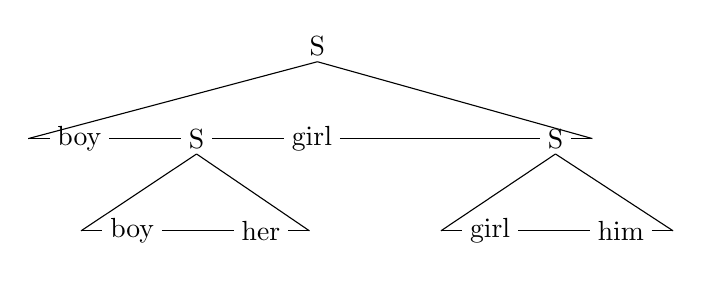
\begin{tikzpicture}
\node at (0.000000, 0.000000) {S};
\node at (-3.023544, -1.171530) {boy};
\node at (-1.534714, -1.171530) {S};
\node at (-2.352594, -2.343060) {boy};
\node at (-0.716835, -2.343060) {her};
\node at (-0.069804, -1.171530) {girl};
\node at (3.023544, -1.171530) {S};
\node at (2.193461, -2.343060) {girl};
\node at (3.853627, -2.343060) {him};
\draw (0.000000,-0.195255) -- (-3.672771,-1.171530);
\draw (0.000000,-0.195255) -- (3.492159,-1.171530);
\draw (-3.672771,-1.171530) -- (-3.401784,-1.171530);
\draw (-2.645304,-1.171530) -- (-1.732342,-1.171530);
\draw (-1.337086,-1.171530) -- (-0.424125,-1.171530);
\draw (0.284517,-1.171530) -- (2.825916,-1.171530);
\draw (3.221172,-1.171530) -- (3.492159,-1.171530);
\draw (-1.534714,-1.366785) -- (-3.001821,-2.343060);
\draw (-1.534714,-1.366785) -- (-0.101290,-2.343060);
\draw (-3.001821,-2.343060) -- (-2.730834,-2.343060);
\draw (-1.974354,-2.343060) -- (-1.061393,-2.343060);
\draw (-0.372277,-2.343060) -- (-0.101290,-2.343060);
\draw (3.023544,-1.366785) -- (1.568152,-2.343060);
\draw (3.023544,-1.366785) -- (4.517499,-2.343060);
\draw (1.568152,-2.343060) -- (1.839139,-2.343060);
\draw (2.547782,-2.343060) -- (3.460743,-2.343060);
\draw (4.246512,-2.343060) -- (4.517499,-2.343060);
\end{tikzpicture}
}
\end{minipage}
\bigbreak

\clearpage

%%%%%%%%%%%%%%%%%%%%%%%%%%%%%%%%%%%%%%%%%%%%%%%%%%%%%%%%%%%%%%%%
%
%     (1.2) *John killed herself.
%
%%%%%%%%%%%%%%%%%%%%%%%%%%%%%%%%%%%%%%%%%%%%%%%%%%%%%%%%%%%%%%%%

\section*{(1.2) *John killed herself.}
\addcontentsline{toc}{section}{(1.2) *John killed herself.}

\bigbreak
\begin{enumerate*}
\item[(1.2)] *John killed herself.
\end{enumerate*}
\bigbreak
\bigbreak
\begin{minipage}{\textwidth}
\makebox[\textwidth][c]{
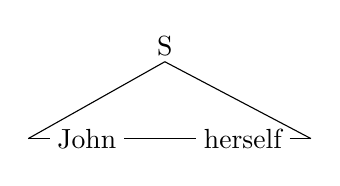
\begin{tikzpicture}
\node at (0.000000, 0.000000) {S};
\node at (-0.990437, -1.171530) {John};
\node at (0.990437, -1.171530) {herself};
\draw (0.000000,-0.195255) -- (-1.734851,-1.171530);
\draw (0.000000,-0.195255) -- (1.855909,-1.171530);
\draw (-1.734851,-1.171530) -- (-1.463864,-1.171530);
\draw (-0.517010,-1.171530) -- (0.395952,-1.171530);
\draw (1.584922,-1.171530) -- (1.855909,-1.171530);
\end{tikzpicture}
}
\end{minipage}
\bigbreak

\clearpage

%%%%%%%%%%%%%%%%%%%%%%%%%%%%%%%%%%%%%%%%%%%%%%%%%%%%%%%%%%%%%%%%
%
%     (1.4) Some students think they are smarter than they are.
%
%%%%%%%%%%%%%%%%%%%%%%%%%%%%%%%%%%%%%%%%%%%%%%%%%%%%%%%%%%%%%%%%

\section*{(1.4) Some students think they are smarter than they are.}
\addcontentsline{toc}{section}{(1.4) Some students think they are smarter than they are.}

\bigbreak
\begin{enumerate*}
\item[(1.4)] Some students think they are smarter than they are.
\end{enumerate*}
\bigbreak
\bigbreak
\begin{minipage}{\textwidth}
\makebox[\textwidth][c]{
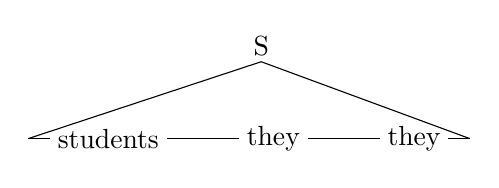
\begin{tikzpicture}
\node at (0.000000, 0.000000) {S};
\node at (-1.941335, -1.171530) {students};
\node at (0.154740, -1.171530) {they};
\node at (1.941335, -1.171530) {they};
\draw (0.000000,-0.195255) -- (-2.958619,-1.171530);
\draw (0.000000,-0.195255) -- (2.649138,-1.171530);
\draw (-2.958619,-1.171530) -- (-2.687631,-1.171530);
\draw (-1.195038,-1.171530) -- (-0.282076,-1.171530);
\draw (0.591557,-1.171530) -- (1.504518,-1.171530);
\draw (2.378151,-1.171530) -- (2.649138,-1.171530);
\end{tikzpicture}
}
\end{minipage}
\bigbreak

\clearpage

%%%%%%%%%%%%%%%%%%%%%%%%%%%%%%%%%%%%%%%%%%%%%%%%%%%%%%%%%%%%%%%%
%
%     (1.6) My uncle has never ridden a camel but his brother has, although it was lame.
%
%%%%%%%%%%%%%%%%%%%%%%%%%%%%%%%%%%%%%%%%%%%%%%%%%%%%%%%%%%%%%%%%

\section*{(1.6) My uncle has never ridden a camel but his brother has, although it was lame.}
\addcontentsline{toc}{section}{(1.6) My uncle has never ridden a camel but his brother has, although it was lame.}

\bigbreak
\begin{enumerate*}
\item[(1.6)] My uncle has never ridden a camel but his brother has, although it was lame.
\end{enumerate*}
\bigbreak
\bigbreak
\begin{minipage}{\textwidth}
\makebox[\textwidth][c]{
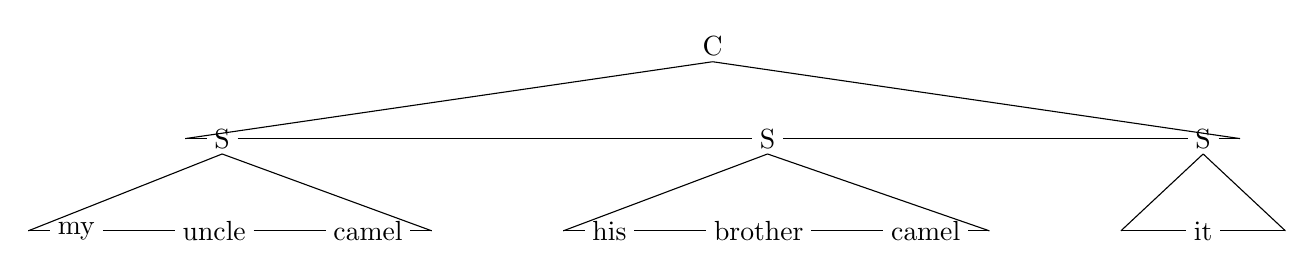
\begin{tikzpicture}
\node at (0.000000, 0.000000) {C};
\node at (-6.229407, -1.171530) {S};
\node at (-8.081900, -2.343060) {my};
\node at (-6.329475, -2.343060) {uncle};
\node at (-4.376913, -2.343060) {camel};
\node at (0.697308, -1.171530) {S};
\node at (-1.310413, -2.343060) {his};
\node at (0.585524, -2.343060) {brother};
\node at (2.705030, -2.343060) {camel};
\node at (6.229407, -1.171530) {S};
\node at (6.229407, -2.343060) {it};
\draw (0.000000,-0.195255) -- (-6.698022,-1.171530);
\draw (0.000000,-0.195255) -- (6.698022,-1.171530);
\draw (-6.698022,-1.171530) -- (-6.427035,-1.171530);
\draw (-6.031778,-1.171530) -- (0.499680,-1.171530);
\draw (0.894936,-1.171530) -- (6.031778,-1.171530);
\draw (6.427035,-1.171530) -- (6.698022,-1.171530);
\draw (-6.229407,-1.366785) -- (-8.692076,-2.343060);
\draw (-6.229407,-1.366785) -- (-3.566600,-2.343060);
\draw (-8.692076,-2.343060) -- (-8.421089,-2.343060);
\draw (-7.742711,-2.343060) -- (-6.829749,-2.343060);
\draw (-5.829201,-2.343060) -- (-4.916239,-2.343060);
\draw (-3.837587,-2.343060) -- (-3.566600,-2.343060);
\draw (0.697308,-1.366785) -- (-1.897158,-2.343060);
\draw (0.697308,-1.366785) -- (3.515343,-2.343060);
\draw (-1.897158,-2.343060) -- (-1.626171,-2.343060);
\draw (-0.994656,-2.343060) -- (-0.081694,-2.343060);
\draw (1.252743,-2.343060) -- (2.165704,-2.343060);
\draw (3.244356,-2.343060) -- (3.515343,-2.343060);
\draw (6.229407,-1.366785) -- (5.184785,-2.343060);
\draw (6.229407,-1.366785) -- (7.274028,-2.343060);
\draw (5.184785,-2.343060) -- (6.012253,-2.343060);
\draw (6.446560,-2.343060) -- (7.274028,-2.343060);
\end{tikzpicture}
}
\end{minipage}
\bigbreak

\clearpage

%%%%%%%%%%%%%%%%%%%%%%%%%%%%%%%%%%%%%%%%%%%%%%%%%%%%%%%%%%%%%%%%
%
%     (1.10) I like the fresh candy better than the stale PHI.
%
%%%%%%%%%%%%%%%%%%%%%%%%%%%%%%%%%%%%%%%%%%%%%%%%%%%%%%%%%%%%%%%%

\section*{(1.10) I like the fresh candy better than the stale PHI.}
\addcontentsline{toc}{section}{(1.10) I like the fresh candy better than the stale PHI.}

\bigbreak
\begin{enumerate*}
\item[(1.10)] I like the fresh candy better than the stale PHI.
\end{enumerate*}
\bigbreak
\bigbreak
\begin{minipage}{\textwidth}
\makebox[\textwidth][c]{
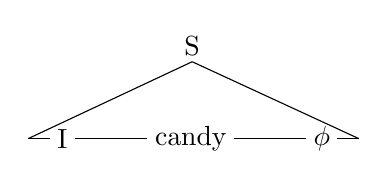
\begin{tikzpicture}
\node at (0.000000, 0.000000) {S};
\node at (-1.647475, -1.171530) {I};
\node at (-0.017085, -1.171530) {candy};
\node at (1.647475, -1.171530) {$\phi$};
\draw (0.000000,-0.195255) -- (-2.081920,-1.171530);
\draw (0.000000,-0.195255) -- (2.116090,-1.171530);
\draw (-2.081920,-1.171530) -- (-1.810933,-1.171530);
\draw (-1.484017,-1.171530) -- (-0.571055,-1.171530);
\draw (0.536885,-1.171530) -- (1.449847,-1.171530);
\draw (1.845103,-1.171530) -- (2.116090,-1.171530);
\end{tikzpicture}
}
\end{minipage}
\bigbreak

\clearpage

%%%%%%%%%%%%%%%%%%%%%%%%%%%%%%%%%%%%%%%%%%%%%%%%%%%%%%%%%%%%%%%%
%
%     (1.11) If John can, he will do it.
%
%%%%%%%%%%%%%%%%%%%%%%%%%%%%%%%%%%%%%%%%%%%%%%%%%%%%%%%%%%%%%%%%

\section*{(1.11) If John can, he will do it.}
\addcontentsline{toc}{section}{(1.11) If John can, he will do it.}

\bigbreak
\begin{enumerate*}
\item[(1.11)] If John can, he will do it.
\end{enumerate*}
\bigbreak
\bigbreak
\begin{minipage}{\textwidth}
\makebox[\textwidth][c]{
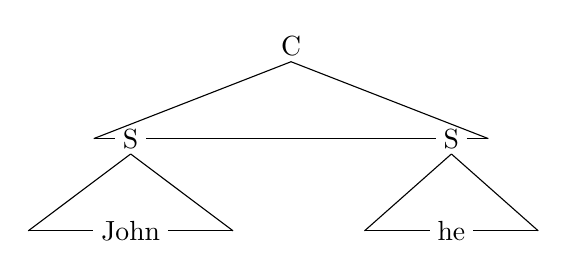
\begin{tikzpicture}
\node at (0.000000, 0.000000) {C};
\node at (-2.036768, -1.171530) {S};
\node at (-2.036768, -2.343060) {John};
\node at (2.036768, -1.171530) {S};
\node at (2.036768, -2.343060) {he};
\draw (0.000000,-0.195255) -- (-2.505383,-1.171530);
\draw (0.000000,-0.195255) -- (2.505383,-1.171530);
\draw (-2.505383,-1.171530) -- (-2.234396,-1.171530);
\draw (-1.839140,-1.171530) -- (1.839140,-1.171530);
\draw (2.234396,-1.171530) -- (2.505383,-1.171530);
\draw (-2.036768,-1.366785) -- (-3.337663,-2.343060);
\draw (-2.036768,-1.366785) -- (-0.735872,-2.343060);
\draw (-3.337663,-2.343060) -- (-2.510195,-2.343060);
\draw (-1.563340,-2.343060) -- (-0.735872,-2.343060);
\draw (2.036768,-1.366785) -- (0.933570,-2.343060);
\draw (2.036768,-1.366785) -- (3.139966,-2.343060);
\draw (0.933570,-2.343060) -- (1.761037,-2.343060);
\draw (2.312498,-2.343060) -- (3.139966,-2.343060);
\end{tikzpicture}
}
\end{minipage}
\bigbreak

\clearpage

%%%%%%%%%%%%%%%%%%%%%%%%%%%%%%%%%%%%%%%%%%%%%%%%%%%%%%%%%%%%%%%%
%
%     (1.12) If he can, John will do it.
%
%%%%%%%%%%%%%%%%%%%%%%%%%%%%%%%%%%%%%%%%%%%%%%%%%%%%%%%%%%%%%%%%

\section*{(1.12) If he can, John will do it.}
\addcontentsline{toc}{section}{(1.12) If he can, John will do it.}

\bigbreak
\begin{enumerate*}
\item[(1.12)] If he can, John will do it.
\end{enumerate*}
\bigbreak
\bigbreak
\begin{minipage}{\textwidth}
\makebox[\textwidth][c]{
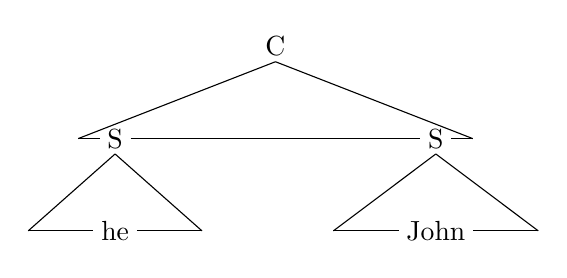
\begin{tikzpicture}
\node at (0.000000, 0.000000) {C};
\node at (-2.036768, -1.171530) {S};
\node at (-2.036768, -2.343060) {he};
\node at (2.036768, -1.171530) {S};
\node at (2.036768, -2.343060) {John};
\draw (0.000000,-0.195255) -- (-2.505383,-1.171530);
\draw (0.000000,-0.195255) -- (2.505383,-1.171530);
\draw (-2.505383,-1.171530) -- (-2.234396,-1.171530);
\draw (-1.839140,-1.171530) -- (1.839140,-1.171530);
\draw (2.234396,-1.171530) -- (2.505383,-1.171530);
\draw (-2.036768,-1.366785) -- (-3.139966,-2.343060);
\draw (-2.036768,-1.366785) -- (-0.933570,-2.343060);
\draw (-3.139966,-2.343060) -- (-2.312498,-2.343060);
\draw (-1.761037,-2.343060) -- (-0.933570,-2.343060);
\draw (2.036768,-1.366785) -- (0.735872,-2.343060);
\draw (2.036768,-1.366785) -- (3.337663,-2.343060);
\draw (0.735872,-2.343060) -- (1.563340,-2.343060);
\draw (2.510195,-2.343060) -- (3.337663,-2.343060);
\end{tikzpicture}
}
\end{minipage}
\bigbreak

\clearpage

%%%%%%%%%%%%%%%%%%%%%%%%%%%%%%%%%%%%%%%%%%%%%%%%%%%%%%%%%%%%%%%%
%
%     (1.13) John will do it if he can.
%
%%%%%%%%%%%%%%%%%%%%%%%%%%%%%%%%%%%%%%%%%%%%%%%%%%%%%%%%%%%%%%%%

\section*{(1.13) John will do it if he can.}
\addcontentsline{toc}{section}{(1.13) John will do it if he can.}

\bigbreak
\begin{enumerate*}
\item[(1.13)] John will do it if he can.
\end{enumerate*}
\bigbreak
\bigbreak
\begin{minipage}{\textwidth}
\makebox[\textwidth][c]{
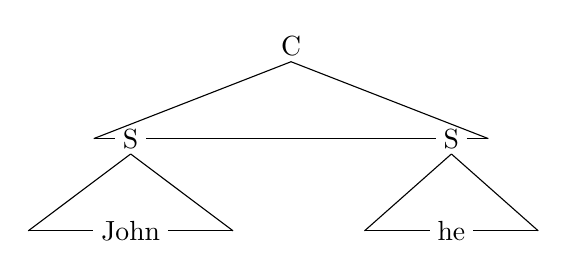
\begin{tikzpicture}
\node at (0.000000, 0.000000) {C};
\node at (-2.036768, -1.171530) {S};
\node at (-2.036768, -2.343060) {John};
\node at (2.036768, -1.171530) {S};
\node at (2.036768, -2.343060) {he};
\draw (0.000000,-0.195255) -- (-2.505383,-1.171530);
\draw (0.000000,-0.195255) -- (2.505383,-1.171530);
\draw (-2.505383,-1.171530) -- (-2.234396,-1.171530);
\draw (-1.839140,-1.171530) -- (1.839140,-1.171530);
\draw (2.234396,-1.171530) -- (2.505383,-1.171530);
\draw (-2.036768,-1.366785) -- (-3.337663,-2.343060);
\draw (-2.036768,-1.366785) -- (-0.735872,-2.343060);
\draw (-3.337663,-2.343060) -- (-2.510195,-2.343060);
\draw (-1.563340,-2.343060) -- (-0.735872,-2.343060);
\draw (2.036768,-1.366785) -- (0.933570,-2.343060);
\draw (2.036768,-1.366785) -- (3.139966,-2.343060);
\draw (0.933570,-2.343060) -- (1.761037,-2.343060);
\draw (2.312498,-2.343060) -- (3.139966,-2.343060);
\end{tikzpicture}
}
\end{minipage}
\bigbreak

\clearpage

%%%%%%%%%%%%%%%%%%%%%%%%%%%%%%%%%%%%%%%%%%%%%%%%%%%%%%%%%%%%%%%%
%
%     (1.14) He will do it if John can.
%
%%%%%%%%%%%%%%%%%%%%%%%%%%%%%%%%%%%%%%%%%%%%%%%%%%%%%%%%%%%%%%%%

\section*{(1.14) He will do it if John can.}
\addcontentsline{toc}{section}{(1.14) He will do it if John can.}

\bigbreak
\begin{enumerate*}
\item[(1.14)] He will do it if John can.
\end{enumerate*}
\bigbreak
\bigbreak
\begin{minipage}{\textwidth}
\makebox[\textwidth][c]{
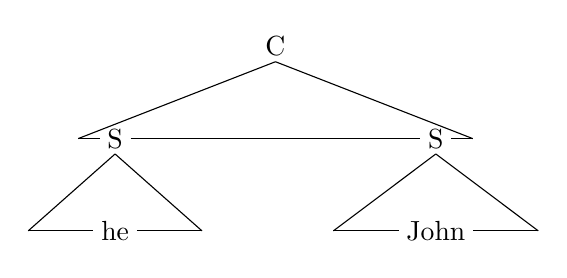
\begin{tikzpicture}
\node at (0.000000, 0.000000) {C};
\node at (-2.036768, -1.171530) {S};
\node at (-2.036768, -2.343060) {he};
\node at (2.036768, -1.171530) {S};
\node at (2.036768, -2.343060) {John};
\draw (0.000000,-0.195255) -- (-2.505383,-1.171530);
\draw (0.000000,-0.195255) -- (2.505383,-1.171530);
\draw (-2.505383,-1.171530) -- (-2.234396,-1.171530);
\draw (-1.839140,-1.171530) -- (1.839140,-1.171530);
\draw (2.234396,-1.171530) -- (2.505383,-1.171530);
\draw (-2.036768,-1.366785) -- (-3.139966,-2.343060);
\draw (-2.036768,-1.366785) -- (-0.933570,-2.343060);
\draw (-3.139966,-2.343060) -- (-2.312498,-2.343060);
\draw (-1.761037,-2.343060) -- (-0.933570,-2.343060);
\draw (2.036768,-1.366785) -- (0.735872,-2.343060);
\draw (2.036768,-1.366785) -- (3.337663,-2.343060);
\draw (0.735872,-2.343060) -- (1.563340,-2.343060);
\draw (2.510195,-2.343060) -- (3.337663,-2.343060);
\end{tikzpicture}
}
\end{minipage}
\bigbreak

\clearpage

%%%%%%%%%%%%%%%%%%%%%%%%%%%%%%%%%%%%%%%%%%%%%%%%%%%%%%%%%%%%%%%%
%
%     (1.24) I have a cat at home, but hate it.
%
%%%%%%%%%%%%%%%%%%%%%%%%%%%%%%%%%%%%%%%%%%%%%%%%%%%%%%%%%%%%%%%%

\section*{(1.24) I have a cat at home, but hate it.}
\addcontentsline{toc}{section}{(1.24) I have a cat at home, but hate it.}

\bigbreak
\begin{enumerate*}
\item[(1.24)] I have a cat at home, but hate it.
\end{enumerate*}
\bigbreak
\bigbreak
\begin{minipage}{\textwidth}
\makebox[\textwidth][c]{
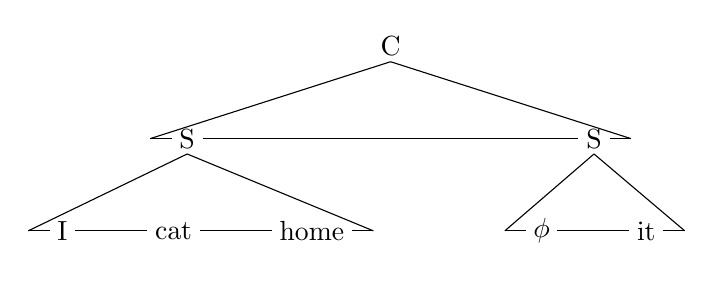
\begin{tikzpicture}
\node at (0.000000, 0.000000) {C};
\node at (-2.583485, -1.171530) {S};
\node at (-4.167501, -2.343060) {I};
\node at (-2.756775, -2.343060) {cat};
\node at (-0.999469, -2.343060) {home};
\node at (2.583485, -1.171530) {S};
\node at (1.919613, -2.343060) {$\phi$};
\node at (3.247356, -2.343060) {it};
\draw (0.000000,-0.195255) -- (-3.052100,-1.171530);
\draw (0.000000,-0.195255) -- (3.052100,-1.171530);
\draw (-3.052100,-1.171530) -- (-2.781113,-1.171530);
\draw (-2.385857,-1.171530) -- (2.385857,-1.171530);
\draw (2.781113,-1.171530) -- (3.052100,-1.171530);
\draw (-2.583485,-1.366785) -- (-4.601946,-2.343060);
\draw (-2.583485,-1.366785) -- (-0.218444,-2.343060);
\draw (-4.601946,-2.343060) -- (-4.330959,-2.343060);
\draw (-4.004043,-2.343060) -- (-3.091082,-2.343060);
\draw (-2.422468,-2.343060) -- (-1.509506,-2.343060);
\draw (-0.489431,-2.343060) -- (-0.218444,-2.343060);
\draw (2.583485,-1.366785) -- (1.450998,-2.343060);
\draw (2.583485,-1.366785) -- (3.735497,-2.343060);
\draw (1.450998,-2.343060) -- (1.721985,-2.343060);
\draw (2.117241,-2.343060) -- (3.030203,-2.343060);
\draw (3.464510,-2.343060) -- (3.735497,-2.343060);
\end{tikzpicture}
}
\end{minipage}
\bigbreak

\clearpage

%%%%%%%%%%%%%%%%%%%%%%%%%%%%%%%%%%%%%%%%%%%%%%%%%%%%%%%%%%%%%%%%
%
%     (1.25) I want to get a cat for myself.
%
%%%%%%%%%%%%%%%%%%%%%%%%%%%%%%%%%%%%%%%%%%%%%%%%%%%%%%%%%%%%%%%%

\section*{(1.25) I want to get a cat for myself.}
\addcontentsline{toc}{section}{(1.25) I want to get a cat for myself.}

\bigbreak
\begin{enumerate*}
\item[(1.25)] I want to get a cat for myself.
\end{enumerate*}
\bigbreak
\bigbreak
\begin{minipage}{\textwidth}
\makebox[\textwidth][c]{
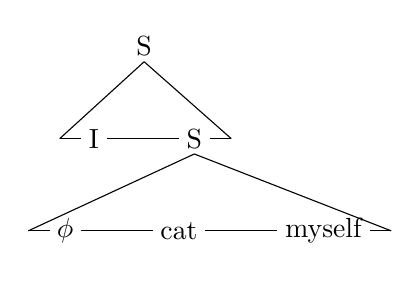
\begin{tikzpicture}
\node at (0.000000, 0.000000) {S};
\node at (-0.637024, -1.171530) {I};
\node at (0.637024, -1.171530) {S};
\node at (-1.003617, -2.343060) {$\phi$};
\node at (0.441280, -2.343060) {cat};
\node at (2.277664, -2.343060) {myself};
\draw (0.000000,-0.195255) -- (-1.071469,-1.171530);
\draw (0.000000,-0.195255) -- (1.105639,-1.171530);
\draw (-1.071469,-1.171530) -- (-0.800482,-1.171530);
\draw (-0.473566,-1.171530) -- (0.439396,-1.171530);
\draw (0.834652,-1.171530) -- (1.105639,-1.171530);
\draw (0.637024,-1.366785) -- (-1.472232,-2.343060);
\draw (0.637024,-1.366785) -- (3.137768,-2.343060);
\draw (-1.472232,-2.343060) -- (-1.201245,-2.343060);
\draw (-0.805989,-2.343060) -- (0.106972,-2.343060);
\draw (0.775587,-2.343060) -- (1.688548,-2.343060);
\draw (2.866781,-2.343060) -- (3.137768,-2.343060);
\end{tikzpicture}
}
\end{minipage}
\bigbreak

\clearpage

%%%%%%%%%%%%%%%%%%%%%%%%%%%%%%%%%%%%%%%%%%%%%%%%%%%%%%%%%%%%%%%%
%
%     (1.27) The men took off their hats.
%
%%%%%%%%%%%%%%%%%%%%%%%%%%%%%%%%%%%%%%%%%%%%%%%%%%%%%%%%%%%%%%%%

\section*{(1.27) The men took off their hats.}
\addcontentsline{toc}{section}{(1.27) The men took off their hats.}

\bigbreak
\begin{enumerate*}
\item[(1.27)] The men took off their hats.
\end{enumerate*}
\bigbreak
\bigbreak
\begin{minipage}{\textwidth}
\makebox[\textwidth][c]{
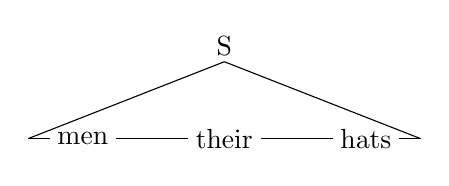
\begin{tikzpicture}
\node at (0.000000, 0.000000) {S};
\node at (-1.797333, -1.171530) {men};
\node at (-0.000488, -1.171530) {their};
\node at (1.797333, -1.171530) {hats};
\draw (0.000000,-0.195255) -- (-2.490493,-1.171530);
\draw (0.000000,-0.195255) -- (2.491469,-1.171530);
\draw (-2.490493,-1.171530) -- (-2.219506,-1.171530);
\draw (-1.375161,-1.171530) -- (-0.462200,-1.171530);
\draw (0.461223,-1.171530) -- (1.374185,-1.171530);
\draw (2.220482,-1.171530) -- (2.491469,-1.171530);
\end{tikzpicture}
}
\end{minipage}
\bigbreak

\clearpage

%%%%%%%%%%%%%%%%%%%%%%%%%%%%%%%%%%%%%%%%%%%%%%%%%%%%%%%%%%%%%%%%
%
%     (1.51) The man who lives next door said that he would mow my lawn.
%
%%%%%%%%%%%%%%%%%%%%%%%%%%%%%%%%%%%%%%%%%%%%%%%%%%%%%%%%%%%%%%%%

\section*{(1.51) The man who lives next door said that he would mow my lawn.}
\addcontentsline{toc}{section}{(1.51) The man who lives next door said that he would mow my lawn.}

\bigbreak
\begin{enumerate*}
\item[(1.51)] The man who lives next door said that he would mow my lawn.
\end{enumerate*}
\bigbreak
\bigbreak
\begin{minipage}{\textwidth}
\makebox[\textwidth][c]{
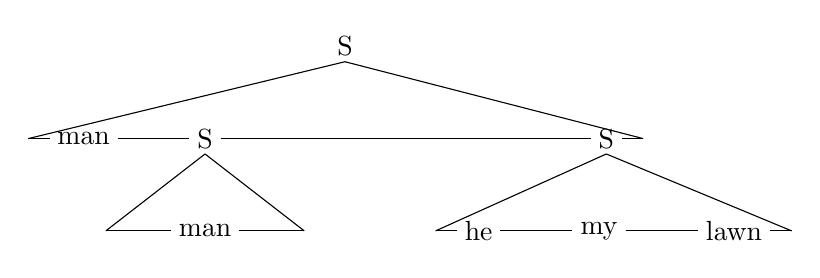
\begin{tikzpicture}
\node at (0.000000, 0.000000) {S};
\node at (-3.319357, -1.171530) {man};
\node at (-1.776832, -1.171530) {S};
\node at (-1.776832, -2.343060) {man};
\node at (3.319357, -1.171530) {S};
\node at (1.698730, -2.343060) {he};
\node at (3.226611, -2.343060) {my};
\node at (4.939985, -2.343060) {lawn};
\draw (0.000000,-0.195255) -- (-4.022280,-1.171530);
\draw (0.000000,-0.195255) -- (3.787973,-1.171530);
\draw (-4.022280,-1.171530) -- (-3.751293,-1.171530);
\draw (-2.887422,-1.171530) -- (-1.974461,-1.171530);
\draw (-1.579204,-1.171530) -- (3.121729,-1.171530);
\draw (3.516985,-1.171530) -- (3.787973,-1.171530);
\draw (-1.776832,-1.366785) -- (-3.036236,-2.343060);
\draw (-1.776832,-1.366785) -- (-0.517429,-2.343060);
\draw (-3.036236,-2.343060) -- (-2.208768,-2.343060);
\draw (-1.344897,-2.343060) -- (-0.517429,-2.343060);
\draw (3.319357,-1.366785) -- (1.152013,-2.343060);
\draw (3.319357,-1.366785) -- (5.672195,-2.343060);
\draw (1.152013,-2.343060) -- (1.423000,-2.343060);
\draw (1.974460,-2.343060) -- (2.887422,-2.343060);
\draw (3.565800,-2.343060) -- (4.478761,-2.343060);
\draw (5.401208,-2.343060) -- (5.672195,-2.343060);
\end{tikzpicture}
}
\end{minipage}
\bigbreak

\clearpage

%%%%%%%%%%%%%%%%%%%%%%%%%%%%%%%%%%%%%%%%%%%%%%%%%%%%%%%%%%%%%%%%
%
%     (1.52) Somebody seduced Bill's sister, but no one will ever seduce Jack’s and she knows it.
%
%%%%%%%%%%%%%%%%%%%%%%%%%%%%%%%%%%%%%%%%%%%%%%%%%%%%%%%%%%%%%%%%

\section*{(1.52) Somebody seduced Bill's sister, but no one will ever seduce Jack’s and she knows it.}
\addcontentsline{toc}{section}{(1.52) Somebody seduced Bill's sister, but no one will ever seduce Jack’s and she knows it.}

\bigbreak
\begin{enumerate*}
\item[(1.52)] Somebody seduced Bill's sister, but no one will ever seduce Jack’s and she knows it.
\end{enumerate*}
\bigbreak
\bigbreak
\begin{minipage}{\textwidth}
\makebox[\textwidth][c]{
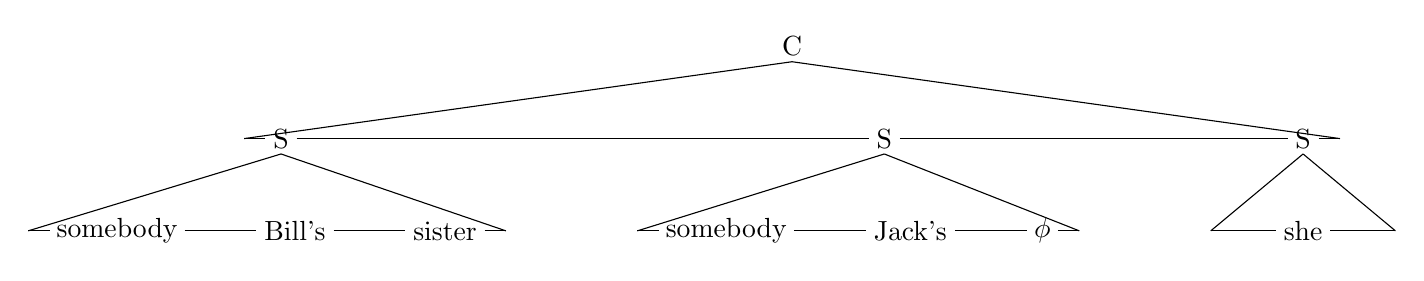
\begin{tikzpicture}
\node at (0.000000, 0.000000) {C};
\node at (-6.489951, -1.171530) {S};
\node at (-8.572115, -2.343060) {somebody};
\node at (-6.312512, -2.343060) {Bill's};
\node at (-4.407788, -2.343060) {sister};
\node at (1.171659, -1.171530) {S};
\node at (-0.836063, -2.343060) {somebody};
\node at (1.501641, -2.343060) {Jack's};
\node at (3.179381, -2.343060) {$\phi$};
\node at (6.489951, -1.171530) {S};
\node at (6.489951, -2.343060) {she};
\draw (0.000000,-0.195255) -- (-6.958567,-1.171530);
\draw (0.000000,-0.195255) -- (6.958567,-1.171530);
\draw (-6.958567,-1.171530) -- (-6.687579,-1.171530);
\draw (-6.292323,-1.171530) -- (0.974031,-1.171530);
\draw (1.369287,-1.171530) -- (6.292323,-1.171530);
\draw (6.687579,-1.171530) -- (6.958567,-1.171530);
\draw (-6.489951,-1.366785) -- (-9.700695,-2.343060);
\draw (-6.489951,-1.366785) -- (-3.634086,-2.343060);
\draw (-9.700695,-2.343060) -- (-9.429708,-2.343060);
\draw (-7.714521,-2.343060) -- (-6.801560,-2.343060);
\draw (-5.823464,-2.343060) -- (-4.910503,-2.343060);
\draw (-3.905073,-2.343060) -- (-3.634086,-2.343060);
\draw (1.171659,-1.366785) -- (-1.964644,-2.343060);
\draw (1.171659,-1.366785) -- (3.647996,-2.343060);
\draw (-1.964644,-2.343060) -- (-1.693657,-2.343060);
\draw (0.021530,-2.343060) -- (0.934491,-2.343060);
\draw (2.068791,-2.343060) -- (2.981753,-2.343060);
\draw (3.377009,-2.343060) -- (3.647996,-2.343060);
\draw (6.489951,-1.366785) -- (5.317438,-2.343060);
\draw (6.489951,-1.366785) -- (7.662465,-2.343060);
\draw (5.317438,-2.343060) -- (6.144906,-2.343060);
\draw (6.834997,-2.343060) -- (7.662465,-2.343060);
\end{tikzpicture}
}
\end{minipage}
\bigbreak

\clearpage

%%%%%%%%%%%%%%%%%%%%%%%%%%%%%%%%%%%%%%%%%%%%%%%%%%%%%%%%%%%%%%%%
%
%     (1.66) Realizing that he was unpopular didn't disturb Oscar.
%
%%%%%%%%%%%%%%%%%%%%%%%%%%%%%%%%%%%%%%%%%%%%%%%%%%%%%%%%%%%%%%%%

\section*{(1.66) Realizing that he was unpopular didn't disturb Oscar.}
\addcontentsline{toc}{section}{(1.66) Realizing that he was unpopular didn't disturb Oscar.}

\bigbreak
\begin{enumerate*}
\item[(1.66)] Realizing that he was unpopular didn't disturb Oscar.
\end{enumerate*}
\bigbreak
\bigbreak
\begin{minipage}{\textwidth}
\makebox[\textwidth][c]{
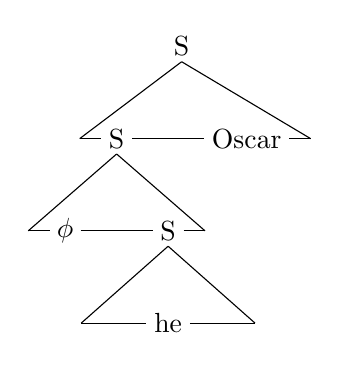
\begin{tikzpicture}
\node at (0.000000, 0.000000) {S};
\node at (-0.825690, -1.171530) {S};
\node at (-1.479798, -2.343060) {$\phi$};
\node at (-0.171581, -2.343060) {S};
\node at (-0.171581, -3.514590) {he};
\node at (0.825690, -1.171530) {Oscar};
\draw (0.000000,-0.195255) -- (-1.294305,-1.171530);
\draw (0.000000,-0.195255) -- (1.637467,-1.171530);
\draw (-1.294305,-1.171530) -- (-1.023318,-1.171530);
\draw (-0.628062,-1.171530) -- (0.284900,-1.171530);
\draw (1.366480,-1.171530) -- (1.637467,-1.171530);
\draw (-0.825690,-1.366785) -- (-1.948414,-2.343060);
\draw (-0.825690,-1.366785) -- (0.297034,-2.343060);
\draw (-1.948414,-2.343060) -- (-1.677426,-2.343060);
\draw (-1.282170,-2.343060) -- (-0.369209,-2.343060);
\draw (0.026047,-2.343060) -- (0.297034,-2.343060);
\draw (-0.171581,-2.538315) -- (-1.274779,-3.514590);
\draw (-0.171581,-2.538315) -- (0.931617,-3.514590);
\draw (-1.274779,-3.514590) -- (-0.447311,-3.514590);
\draw (0.104149,-3.514590) -- (0.931617,-3.514590);
\end{tikzpicture}
}
\end{minipage}
\bigbreak

\clearpage

%%%%%%%%%%%%%%%%%%%%%%%%%%%%%%%%%%%%%%%%%%%%%%%%%%%%%%%%%%%%%%%%
%
%     (1.70) My neighbor who is pregnant said that she was very happy.
%
%%%%%%%%%%%%%%%%%%%%%%%%%%%%%%%%%%%%%%%%%%%%%%%%%%%%%%%%%%%%%%%%

\section*{(1.70) My neighbor who is pregnant said that she was very happy.}
\addcontentsline{toc}{section}{(1.70) My neighbor who is pregnant said that she was very happy.}

\bigbreak
\begin{enumerate*}
\item[(1.70)] My neighbor who is pregnant said that she was very happy.
\end{enumerate*}
\bigbreak
\bigbreak
\begin{minipage}{\textwidth}
\makebox[\textwidth][c]{
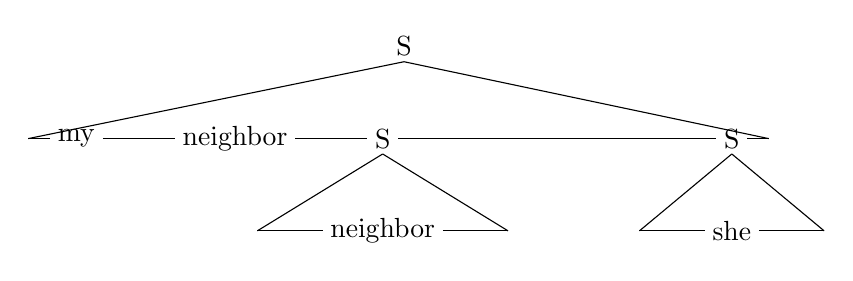
\begin{tikzpicture}
\node at (0.000000, 0.000000) {S};
\node at (-4.162620, -1.171530) {my};
\node at (-2.146111, -1.171530) {neighbor};
\node at (-0.271163, -1.171530) {S};
\node at (-0.271163, -2.343060) {neighbor};
\node at (4.162620, -1.171530) {S};
\node at (4.162620, -2.343060) {she};
\draw (0.000000,-0.195255) -- (-4.772796,-1.171530);
\draw (0.000000,-0.195255) -- (4.631235,-1.171530);
\draw (-4.772796,-1.171530) -- (-4.501808,-1.171530);
\draw (-3.823431,-1.171530) -- (-2.910469,-1.171530);
\draw (-1.381752,-1.171530) -- (-0.468791,-1.171530);
\draw (-0.073535,-1.171530) -- (3.964992,-1.171530);
\draw (4.360248,-1.171530) -- (4.631235,-1.171530);
\draw (-0.271163,-1.366785) -- (-1.862989,-2.343060);
\draw (-0.271163,-1.366785) -- (1.320664,-2.343060);
\draw (-1.862989,-2.343060) -- (-1.035521,-2.343060);
\draw (0.493196,-2.343060) -- (1.320664,-2.343060);
\draw (4.162620,-1.366785) -- (2.990106,-2.343060);
\draw (4.162620,-1.366785) -- (5.335133,-2.343060);
\draw (2.990106,-2.343060) -- (3.817574,-2.343060);
\draw (4.507665,-2.343060) -- (5.335133,-2.343060);
\end{tikzpicture}
}
\end{minipage}
\bigbreak

\clearpage

%%%%%%%%%%%%%%%%%%%%%%%%%%%%%%%%%%%%%%%%%%%%%%%%%%%%%%%%%%%%%%%%
%
%     (1.74) The pilot who shot at it hit the Mig that chased him.
%
%%%%%%%%%%%%%%%%%%%%%%%%%%%%%%%%%%%%%%%%%%%%%%%%%%%%%%%%%%%%%%%%

\section*{(1.74) The pilot who shot at it hit the Mig that chased him.}
\addcontentsline{toc}{section}{(1.74) The pilot who shot at it hit the Mig that chased him.}

\bigbreak
\begin{enumerate*}
\item[(1.74)] The pilot who shot at it hit the Mig that chased him.
\end{enumerate*}
\bigbreak
\bigbreak
\begin{minipage}{\textwidth}
\makebox[\textwidth][c]{
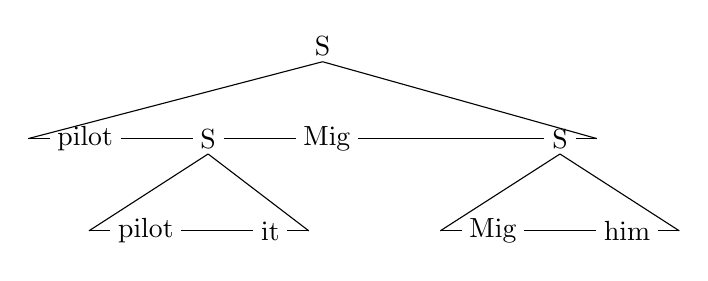
\begin{tikzpicture}
\node at (0.000000, 0.000000) {S};
\node at (-3.015490, -1.171530) {pilot};
\node at (-1.453439, -1.171530) {S};
\node at (-2.244228, -2.343060) {pilot};
\node at (-0.662651, -2.343060) {it};
\node at (0.054916, -1.171530) {Mig};
\node at (3.015490, -1.171530) {S};
\node at (2.163684, -2.343060) {Mig};
\node at (3.867296, -2.343060) {him};
\draw (0.000000,-0.195255) -- (-3.737938,-1.171530);
\draw (0.000000,-0.195255) -- (3.484105,-1.171530);
\draw (-3.737938,-1.171530) -- (-3.466951,-1.171530);
\draw (-2.564029,-1.171530) -- (-1.651067,-1.171530);
\draw (-1.255811,-1.171530) -- (-0.342850,-1.171530);
\draw (0.452681,-1.171530) -- (2.817862,-1.171530);
\draw (3.213118,-1.171530) -- (3.484105,-1.171530);
\draw (-1.453439,-1.366785) -- (-2.966676,-2.343060);
\draw (-1.453439,-1.366785) -- (-0.174510,-2.343060);
\draw (-2.966676,-2.343060) -- (-2.695689,-2.343060);
\draw (-1.792766,-2.343060) -- (-0.879805,-2.343060);
\draw (-0.445498,-2.343060) -- (-0.174510,-2.343060);
\draw (3.015490,-1.366785) -- (1.494932,-2.343060);
\draw (3.015490,-1.366785) -- (4.531167,-2.343060);
\draw (1.494932,-2.343060) -- (1.765919,-2.343060);
\draw (2.561450,-2.343060) -- (3.474411,-2.343060);
\draw (4.260180,-2.343060) -- (4.531167,-2.343060);
\end{tikzpicture}
}
\end{minipage}
\bigbreak

\clearpage

%%%%%%%%%%%%%%%%%%%%%%%%%%%%%%%%%%%%%%%%%%%%%%%%%%%%%%%%%%%%%%%%
%
%     (1.86) The mosquito which bit Algernon was killed by him.
%
%%%%%%%%%%%%%%%%%%%%%%%%%%%%%%%%%%%%%%%%%%%%%%%%%%%%%%%%%%%%%%%%

\section*{(1.86) The mosquito which bit Algernon was killed by him.}
\addcontentsline{toc}{section}{(1.86) The mosquito which bit Algernon was killed by him.}

\bigbreak
\begin{enumerate*}
\item[(1.86)] The mosquito which bit Algernon was killed by him.
\end{enumerate*}
\bigbreak
\bigbreak
\begin{minipage}{\textwidth}
\makebox[\textwidth][c]{
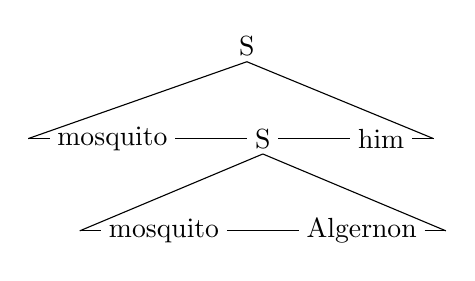
\begin{tikzpicture}
\node at (0.000000, 0.000000) {S};
\node at (-1.706540, -1.171530) {mosquito};
\node at (0.203066, -1.171530) {S};
\node at (-1.052187, -2.343060) {mosquito};
\node at (1.458320, -2.343060) {Algernon};
\node at (1.706540, -1.171530) {him};
\draw (0.000000,-0.195255) -- (-2.776544,-1.171530);
\draw (0.000000,-0.195255) -- (2.370411,-1.171530);
\draw (-2.776544,-1.171530) -- (-2.505557,-1.171530);
\draw (-0.907523,-1.171530) -- (0.005438,-1.171530);
\draw (0.400694,-1.171530) -- (1.313656,-1.171530);
\draw (2.099424,-1.171530) -- (2.370411,-1.171530);
\draw (0.203066,-1.366785) -- (-2.122191,-2.343060);
\draw (0.203066,-1.366785) -- (2.527835,-2.343060);
\draw (-2.122191,-2.343060) -- (-1.851204,-2.343060);
\draw (-0.253170,-2.343060) -- (0.659791,-2.343060);
\draw (2.256848,-2.343060) -- (2.527835,-2.343060);
\end{tikzpicture}
}
\end{minipage}
\bigbreak

\clearpage

%%%%%%%%%%%%%%%%%%%%%%%%%%%%%%%%%%%%%%%%%%%%%%%%%%%%%%%%%%%%%%%%
%
%     (1.87) The mosquito which bit him was killed by Algernon.
%
%%%%%%%%%%%%%%%%%%%%%%%%%%%%%%%%%%%%%%%%%%%%%%%%%%%%%%%%%%%%%%%%

\section*{(1.87) The mosquito which bit him was killed by Algernon.}
\addcontentsline{toc}{section}{(1.87) The mosquito which bit him was killed by Algernon.}

\bigbreak
\begin{enumerate*}
\item[(1.87)] The mosquito which bit him was killed by Algernon.
\end{enumerate*}
\bigbreak
\bigbreak
\begin{minipage}{\textwidth}
\makebox[\textwidth][c]{
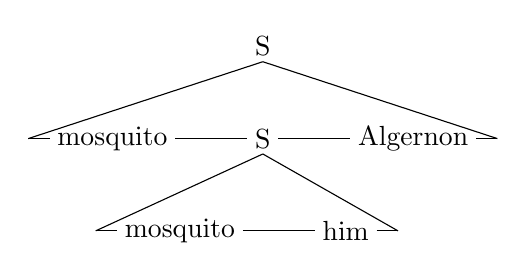
\begin{tikzpicture}
\node at (0.000000, 0.000000) {S};
\node at (-1.909362, -1.171530) {mosquito};
\node at (0.000244, -1.171530) {S};
\node at (-1.052187, -2.343060) {mosquito};
\node at (1.052675, -2.343060) {him};
\node at (1.909362, -1.171530) {Algernon};
\draw (0.000000,-0.195255) -- (-2.979366,-1.171530);
\draw (0.000000,-0.195255) -- (2.978878,-1.171530);
\draw (-2.979366,-1.171530) -- (-2.708379,-1.171530);
\draw (-1.110345,-1.171530) -- (-0.197384,-1.171530);
\draw (0.197872,-1.171530) -- (1.110834,-1.171530);
\draw (2.707891,-1.171530) -- (2.978878,-1.171530);
\draw (0.000244,-1.366785) -- (-2.122191,-2.343060);
\draw (0.000244,-1.366785) -- (1.716547,-2.343060);
\draw (-2.122191,-2.343060) -- (-1.851204,-2.343060);
\draw (-0.253170,-2.343060) -- (0.659791,-2.343060);
\draw (1.445560,-2.343060) -- (1.716547,-2.343060);
\end{tikzpicture}
}
\end{minipage}
\bigbreak

\clearpage

%%%%%%%%%%%%%%%%%%%%%%%%%%%%%%%%%%%%%%%%%%%%%%%%%%%%%%%%%%%%%%%%
%
%     (1.88) Algernon killed the mosquito which bit him.
%
%%%%%%%%%%%%%%%%%%%%%%%%%%%%%%%%%%%%%%%%%%%%%%%%%%%%%%%%%%%%%%%%

\section*{(1.88) Algernon killed the mosquito which bit him.}
\addcontentsline{toc}{section}{(1.88) Algernon killed the mosquito which bit him.}

\bigbreak
\begin{enumerate*}
\item[(1.88)] Algernon killed the mosquito which bit him.
\end{enumerate*}
\bigbreak
\bigbreak
\begin{minipage}{\textwidth}
\makebox[\textwidth][c]{
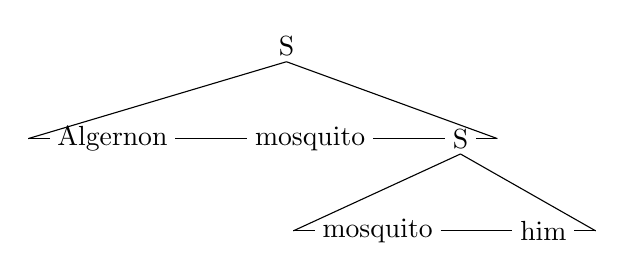
\begin{tikzpicture}
\node at (0.000000, 0.000000) {S};
\node at (-2.210056, -1.171530) {Algernon};
\node at (0.300450, -1.171530) {mosquito};
\node at (2.210056, -1.171530) {S};
\node at (1.157625, -2.343060) {mosquito};
\node at (3.262488, -2.343060) {him};
\draw (0.000000,-0.195255) -- (-3.279572,-1.171530);
\draw (0.000000,-0.195255) -- (2.678672,-1.171530);
\draw (-3.279572,-1.171530) -- (-3.008585,-1.171530);
\draw (-1.411528,-1.171530) -- (-0.498567,-1.171530);
\draw (1.099467,-1.171530) -- (2.012428,-1.171530);
\draw (2.407685,-1.171530) -- (2.678672,-1.171530);
\draw (2.210056,-1.366785) -- (0.087621,-2.343060);
\draw (2.210056,-1.366785) -- (3.926359,-2.343060);
\draw (0.087621,-2.343060) -- (0.358608,-2.343060);
\draw (1.956642,-2.343060) -- (2.869603,-2.343060);
\draw (3.655372,-2.343060) -- (3.926359,-2.343060);
\end{tikzpicture}
}
\end{minipage}
\bigbreak

\clearpage

%%%%%%%%%%%%%%%%%%%%%%%%%%%%%%%%%%%%%%%%%%%%%%%%%%%%%%%%%%%%%%%%
%
%     (1.89) He killed the mosquito which bit Algernon.
%
%%%%%%%%%%%%%%%%%%%%%%%%%%%%%%%%%%%%%%%%%%%%%%%%%%%%%%%%%%%%%%%%

\section*{(1.89) He killed the mosquito which bit Algernon.}
\addcontentsline{toc}{section}{(1.89) He killed the mosquito which bit Algernon.}

\bigbreak
\begin{enumerate*}
\item[(1.89)] He killed the mosquito which bit Algernon.
\end{enumerate*}
\bigbreak
\bigbreak
\begin{minipage}{\textwidth}
\makebox[\textwidth][c]{
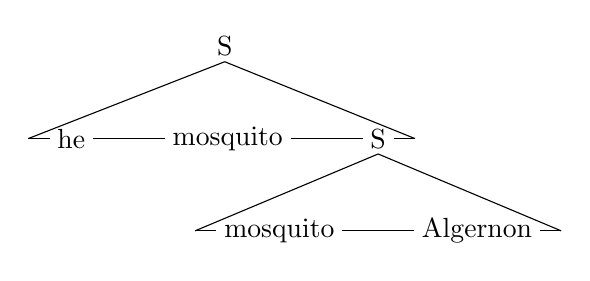
\begin{tikzpicture}
\node at (0.000000, 0.000000) {S};
\node at (-1.948657, -1.171530) {he};
\node at (0.039051, -1.171530) {mosquito};
\node at (1.948657, -1.171530) {S};
\node at (0.693404, -2.343060) {mosquito};
\node at (3.203911, -2.343060) {Algernon};
\draw (0.000000,-0.195255) -- (-2.495375,-1.171530);
\draw (0.000000,-0.195255) -- (2.417272,-1.171530);
\draw (-2.495375,-1.171530) -- (-2.224387,-1.171530);
\draw (-1.672927,-1.171530) -- (-0.759966,-1.171530);
\draw (0.838068,-1.171530) -- (1.751029,-1.171530);
\draw (2.146285,-1.171530) -- (2.417272,-1.171530);
\draw (1.948657,-1.366785) -- (-0.376600,-2.343060);
\draw (1.948657,-1.366785) -- (4.273426,-2.343060);
\draw (-0.376600,-2.343060) -- (-0.105613,-2.343060);
\draw (1.492421,-2.343060) -- (2.405382,-2.343060);
\draw (4.002439,-2.343060) -- (4.273426,-2.343060);
\end{tikzpicture}
}
\end{minipage}
\bigbreak

\clearpage

%%%%%%%%%%%%%%%%%%%%%%%%%%%%%%%%%%%%%%%%%%%%%%%%%%%%%%%%%%%%%%%%
%
%     (1.91) After John Adams woke up, he was hungry.
%
%%%%%%%%%%%%%%%%%%%%%%%%%%%%%%%%%%%%%%%%%%%%%%%%%%%%%%%%%%%%%%%%

\section*{(1.91) After John Adams woke up, he was hungry.}
\addcontentsline{toc}{section}{(1.91) After John Adams woke up, he was hungry.}

\bigbreak
\begin{enumerate*}
\item[(1.91)] After John Adams woke up, he was hungry.
\end{enumerate*}
\bigbreak
\bigbreak
\begin{minipage}{\textwidth}
\makebox[\textwidth][c]{
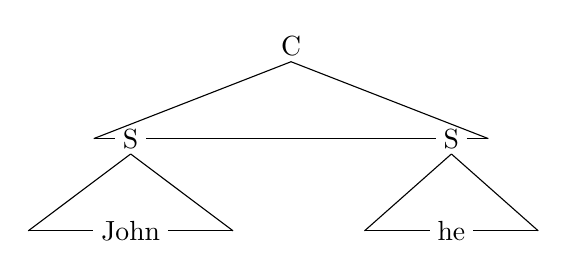
\begin{tikzpicture}
\node at (0.000000, 0.000000) {C};
\node at (-2.036768, -1.171530) {S};
\node at (-2.036768, -2.343060) {John};
\node at (2.036768, -1.171530) {S};
\node at (2.036768, -2.343060) {he};
\draw (0.000000,-0.195255) -- (-2.505383,-1.171530);
\draw (0.000000,-0.195255) -- (2.505383,-1.171530);
\draw (-2.505383,-1.171530) -- (-2.234396,-1.171530);
\draw (-1.839140,-1.171530) -- (1.839140,-1.171530);
\draw (2.234396,-1.171530) -- (2.505383,-1.171530);
\draw (-2.036768,-1.366785) -- (-3.337663,-2.343060);
\draw (-2.036768,-1.366785) -- (-0.735872,-2.343060);
\draw (-3.337663,-2.343060) -- (-2.510195,-2.343060);
\draw (-1.563340,-2.343060) -- (-0.735872,-2.343060);
\draw (2.036768,-1.366785) -- (0.933570,-2.343060);
\draw (2.036768,-1.366785) -- (3.139966,-2.343060);
\draw (0.933570,-2.343060) -- (1.761037,-2.343060);
\draw (2.312498,-2.343060) -- (3.139966,-2.343060);
\end{tikzpicture}
}
\end{minipage}
\bigbreak

\clearpage

%%%%%%%%%%%%%%%%%%%%%%%%%%%%%%%%%%%%%%%%%%%%%%%%%%%%%%%%%%%%%%%%
%
%     (1.92) That Oscar was unpopular didn't disturb him.
%
%%%%%%%%%%%%%%%%%%%%%%%%%%%%%%%%%%%%%%%%%%%%%%%%%%%%%%%%%%%%%%%%

\section*{(1.92) That Oscar was unpopular didn't disturb him.}
\addcontentsline{toc}{section}{(1.92) That Oscar was unpopular didn't disturb him.}

\bigbreak
\begin{enumerate*}
\item[(1.92)] That Oscar was unpopular didn't disturb him.
\end{enumerate*}
\bigbreak
\bigbreak
\begin{minipage}{\textwidth}
\makebox[\textwidth][c]{
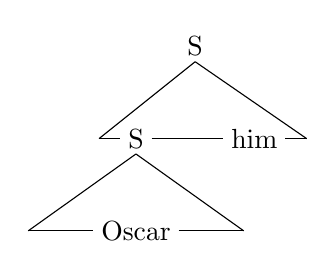
\begin{tikzpicture}
\node at (0.000000, 0.000000) {S};
\node at (-0.751737, -1.171530) {S};
\node at (-0.751737, -2.343060) {Oscar};
\node at (0.751737, -1.171530) {him};
\draw (0.000000,-0.195255) -- (-1.220352,-1.171530);
\draw (0.000000,-0.195255) -- (1.415608,-1.171530);
\draw (-1.220352,-1.171530) -- (-0.949365,-1.171530);
\draw (-0.554109,-1.171530) -- (0.358853,-1.171530);
\draw (1.144621,-1.171530) -- (1.415608,-1.171530);
\draw (-0.751737,-1.366785) -- (-2.119995,-2.343060);
\draw (-0.751737,-1.366785) -- (0.616521,-2.343060);
\draw (-2.119995,-2.343060) -- (-1.292527,-2.343060);
\draw (-0.210947,-2.343060) -- (0.616521,-2.343060);
\end{tikzpicture}
}
\end{minipage}
\bigbreak

\clearpage

%%%%%%%%%%%%%%%%%%%%%%%%%%%%%%%%%%%%%%%%%%%%%%%%%%%%%%%%%%%%%%%%
%
%     (1.93) For your brother to refuse to pay taxes would get him into trouble.
%
%%%%%%%%%%%%%%%%%%%%%%%%%%%%%%%%%%%%%%%%%%%%%%%%%%%%%%%%%%%%%%%%

\section*{(1.93) For your brother to refuse to pay taxes would get him into trouble.}
\addcontentsline{toc}{section}{(1.93) For your brother to refuse to pay taxes would get him into trouble.}

\bigbreak
\begin{enumerate*}
\item[(1.93)] For your brother to refuse to pay taxes would get him into trouble.
\end{enumerate*}
\bigbreak
\bigbreak
\begin{minipage}{\textwidth}
\makebox[\textwidth][c]{
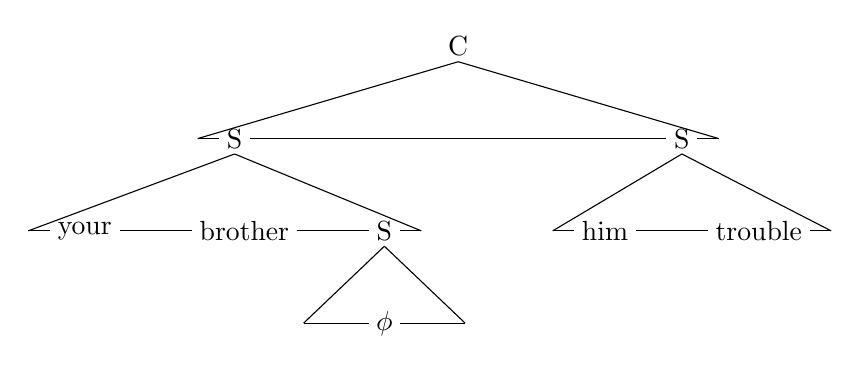
\begin{tikzpicture}
\node at (0.000000, 0.000000) {C};
\node at (-2.840491, -1.171530) {S};
\node at (-4.743019, -2.343060) {your};
\node at (-2.715771, -2.343060) {brother};
\node at (-0.937963, -2.343060) {S};
\node at (-0.937963, -3.514590) {$\phi$};
\node at (2.840491, -1.171530) {S};
\node at (1.863966, -2.343060) {him};
\node at (3.817016, -2.343060) {trouble};
\draw (0.000000,-0.195255) -- (-3.309106,-1.171530);
\draw (0.000000,-0.195255) -- (3.309106,-1.171530);
\draw (-3.309106,-1.171530) -- (-3.038119,-1.171530);
\draw (-2.642863,-1.171530) -- (2.642863,-1.171530);
\draw (3.038119,-1.171530) -- (3.309106,-1.171530);
\draw (-2.840491,-1.366785) -- (-5.461073,-2.343060);
\draw (-2.840491,-1.366785) -- (-0.469348,-2.343060);
\draw (-5.461073,-2.343060) -- (-5.190086,-2.343060);
\draw (-4.295951,-2.343060) -- (-3.382989,-2.343060);
\draw (-2.048552,-2.343060) -- (-1.135591,-2.343060);
\draw (-0.740335,-2.343060) -- (-0.469348,-2.343060);
\draw (-0.937963,-2.538315) -- (-1.963059,-3.514590);
\draw (-0.937963,-2.538315) -- (0.087133,-3.514590);
\draw (-1.963059,-3.514590) -- (-1.135591,-3.514590);
\draw (-0.740335,-3.514590) -- (0.087133,-3.514590);
\draw (2.840491,-1.366785) -- (1.200094,-2.343060);
\draw (2.840491,-1.366785) -- (4.735208,-2.343060);
\draw (1.200094,-2.343060) -- (1.471081,-2.343060);
\draw (2.256850,-2.343060) -- (3.169811,-2.343060);
\draw (4.464221,-2.343060) -- (4.735208,-2.343060);
\end{tikzpicture}
}
\end{minipage}
\bigbreak

\clearpage

%%%%%%%%%%%%%%%%%%%%%%%%%%%%%%%%%%%%%%%%%%%%%%%%%%%%%%%%%%%%%%%%
%
%     (1.94) Anna's complaining about Peter infuriated him.
%
%%%%%%%%%%%%%%%%%%%%%%%%%%%%%%%%%%%%%%%%%%%%%%%%%%%%%%%%%%%%%%%%

\section*{(1.94) Anna's complaining about Peter infuriated him.}
\addcontentsline{toc}{section}{(1.94) Anna's complaining about Peter infuriated him.}

\bigbreak
\begin{enumerate*}
\item[(1.94)] Anna's complaining about Peter infuriated him.
\end{enumerate*}
\bigbreak
\bigbreak
\begin{minipage}{\textwidth}
\makebox[\textwidth][c]{
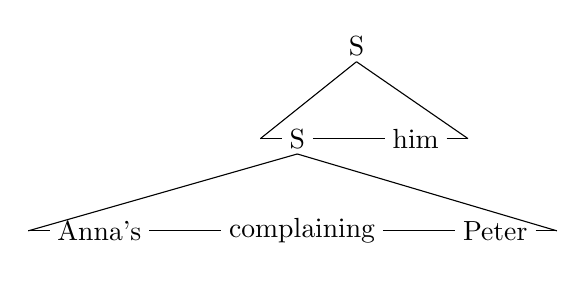
\begin{tikzpicture}
\node at (0.000000, 0.000000) {S};
\node at (-0.751737, -1.171530) {S};
\node at (-3.265172, -2.343060) {Anna's};
\node at (-0.691695, -2.343060) {complaining};
\node at (1.761699, -2.343060) {Peter};
\node at (0.751737, -1.171530) {him};
\draw (0.000000,-0.195255) -- (-1.220352,-1.171530);
\draw (0.000000,-0.195255) -- (1.415608,-1.171530);
\draw (-1.220352,-1.171530) -- (-0.949365,-1.171530);
\draw (-0.554109,-1.171530) -- (0.358853,-1.171530);
\draw (1.144621,-1.171530) -- (1.415608,-1.171530);
\draw (-0.751737,-1.366785) -- (-4.169208,-2.343060);
\draw (-0.751737,-1.366785) -- (2.545652,-2.343060);
\draw (-4.169208,-2.343060) -- (-3.898221,-2.343060);
\draw (-2.632123,-2.343060) -- (-1.719162,-2.343060);
\draw (0.335771,-2.343060) -- (1.248733,-2.343060);
\draw (2.274665,-2.343060) -- (2.545652,-2.343060);
\end{tikzpicture}
}
\end{minipage}
\bigbreak

\clearpage

%%%%%%%%%%%%%%%%%%%%%%%%%%%%%%%%%%%%%%%%%%%%%%%%%%%%%%%%%%%%%%%%
%
%     (1.95) The possibility that Fred will be unpopular doesn’t bother him.
%
%%%%%%%%%%%%%%%%%%%%%%%%%%%%%%%%%%%%%%%%%%%%%%%%%%%%%%%%%%%%%%%%

\section*{(1.95) The possibility that Fred will be unpopular doesn’t bother him.}
\addcontentsline{toc}{section}{(1.95) The possibility that Fred will be unpopular doesn’t bother him.}

\bigbreak
\begin{enumerate*}
\item[(1.95)] The possibility that Fred will be unpopular doesn’t bother him.
\end{enumerate*}
\bigbreak
\bigbreak
\begin{minipage}{\textwidth}
\makebox[\textwidth][c]{
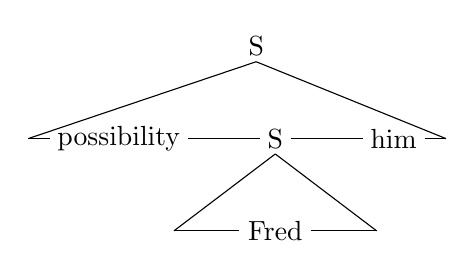
\begin{tikzpicture}
\node at (0.000000, 0.000000) {S};
\node at (-1.746079, -1.171530) {possibility};
\node at (0.242606, -1.171530) {S};
\node at (0.242606, -2.343060) {Fred};
\node at (1.746079, -1.171530) {him};
\draw (0.000000,-0.195255) -- (-2.895162,-1.171530);
\draw (0.000000,-0.195255) -- (2.409951,-1.171530);
\draw (-2.895162,-1.171530) -- (-2.624175,-1.171530);
\draw (-0.867984,-1.171530) -- (0.044978,-1.171530);
\draw (0.440234,-1.171530) -- (1.353195,-1.171530);
\draw (2.138964,-1.171530) -- (2.409951,-1.171530);
\draw (0.242606,-1.366785) -- (-1.044133,-2.343060);
\draw (0.242606,-1.366785) -- (1.529344,-2.343060);
\draw (-1.044133,-2.343060) -- (-0.216665,-2.343060);
\draw (0.701876,-2.343060) -- (1.529344,-2.343060);
\end{tikzpicture}
}
\end{minipage}
\bigbreak

\clearpage

%%%%%%%%%%%%%%%%%%%%%%%%%%%%%%%%%%%%%%%%%%%%%%%%%%%%%%%%%%%%%%%%
%
%     (1.96) After he woke up, John Adams was hungry.
%
%%%%%%%%%%%%%%%%%%%%%%%%%%%%%%%%%%%%%%%%%%%%%%%%%%%%%%%%%%%%%%%%

\section*{(1.96) After he woke up, John Adams was hungry.}
\addcontentsline{toc}{section}{(1.96) After he woke up, John Adams was hungry.}

\bigbreak
\begin{enumerate*}
\item[(1.96)] After he woke up, John Adams was hungry.
\end{enumerate*}
\bigbreak
\bigbreak
\begin{minipage}{\textwidth}
\makebox[\textwidth][c]{
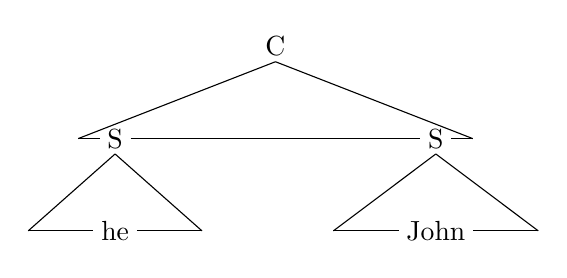
\begin{tikzpicture}
\node at (0.000000, 0.000000) {C};
\node at (-2.036768, -1.171530) {S};
\node at (-2.036768, -2.343060) {he};
\node at (2.036768, -1.171530) {S};
\node at (2.036768, -2.343060) {John};
\draw (0.000000,-0.195255) -- (-2.505383,-1.171530);
\draw (0.000000,-0.195255) -- (2.505383,-1.171530);
\draw (-2.505383,-1.171530) -- (-2.234396,-1.171530);
\draw (-1.839140,-1.171530) -- (1.839140,-1.171530);
\draw (2.234396,-1.171530) -- (2.505383,-1.171530);
\draw (-2.036768,-1.366785) -- (-3.139966,-2.343060);
\draw (-2.036768,-1.366785) -- (-0.933570,-2.343060);
\draw (-3.139966,-2.343060) -- (-2.312498,-2.343060);
\draw (-1.761037,-2.343060) -- (-0.933570,-2.343060);
\draw (2.036768,-1.366785) -- (0.735872,-2.343060);
\draw (2.036768,-1.366785) -- (3.337663,-2.343060);
\draw (0.735872,-2.343060) -- (1.563340,-2.343060);
\draw (2.510195,-2.343060) -- (3.337663,-2.343060);
\end{tikzpicture}
}
\end{minipage}
\bigbreak

\clearpage

%%%%%%%%%%%%%%%%%%%%%%%%%%%%%%%%%%%%%%%%%%%%%%%%%%%%%%%%%%%%%%%%
%
%     (1.97) That he was unpopular didn't disturb Oscar.
%
%%%%%%%%%%%%%%%%%%%%%%%%%%%%%%%%%%%%%%%%%%%%%%%%%%%%%%%%%%%%%%%%

\section*{(1.97) That he was unpopular didn't disturb Oscar.}
\addcontentsline{toc}{section}{(1.97) That he was unpopular didn't disturb Oscar.}

\bigbreak
\begin{enumerate*}
\item[(1.97)] That he was unpopular didn't disturb Oscar.
\end{enumerate*}
\bigbreak
\bigbreak
\begin{minipage}{\textwidth}
\makebox[\textwidth][c]{
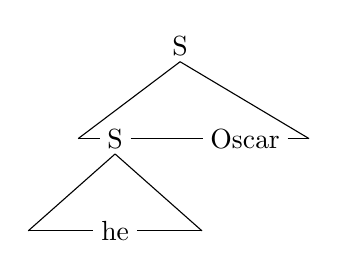
\begin{tikzpicture}
\node at (0.000000, 0.000000) {S};
\node at (-0.825690, -1.171530) {S};
\node at (-0.825690, -2.343060) {he};
\node at (0.825690, -1.171530) {Oscar};
\draw (0.000000,-0.195255) -- (-1.294305,-1.171530);
\draw (0.000000,-0.195255) -- (1.637467,-1.171530);
\draw (-1.294305,-1.171530) -- (-1.023318,-1.171530);
\draw (-0.628062,-1.171530) -- (0.284900,-1.171530);
\draw (1.366480,-1.171530) -- (1.637467,-1.171530);
\draw (-0.825690,-1.366785) -- (-1.928888,-2.343060);
\draw (-0.825690,-1.366785) -- (0.277508,-2.343060);
\draw (-1.928888,-2.343060) -- (-1.101420,-2.343060);
\draw (-0.549960,-2.343060) -- (0.277508,-2.343060);
\end{tikzpicture}
}
\end{minipage}
\bigbreak

\clearpage

%%%%%%%%%%%%%%%%%%%%%%%%%%%%%%%%%%%%%%%%%%%%%%%%%%%%%%%%%%%%%%%%
%
%     (1.98) For him to refuse to pay taxes would get your brother into trouble.
%
%%%%%%%%%%%%%%%%%%%%%%%%%%%%%%%%%%%%%%%%%%%%%%%%%%%%%%%%%%%%%%%%

\section*{(1.98) For him to refuse to pay taxes would get your brother into trouble.}
\addcontentsline{toc}{section}{(1.98) For him to refuse to pay taxes would get your brother into trouble.}

\bigbreak
\begin{enumerate*}
\item[(1.98)] For him to refuse to pay taxes would get your brother into trouble.
\end{enumerate*}
\bigbreak
\bigbreak
\begin{minipage}{\textwidth}
\makebox[\textwidth][c]{
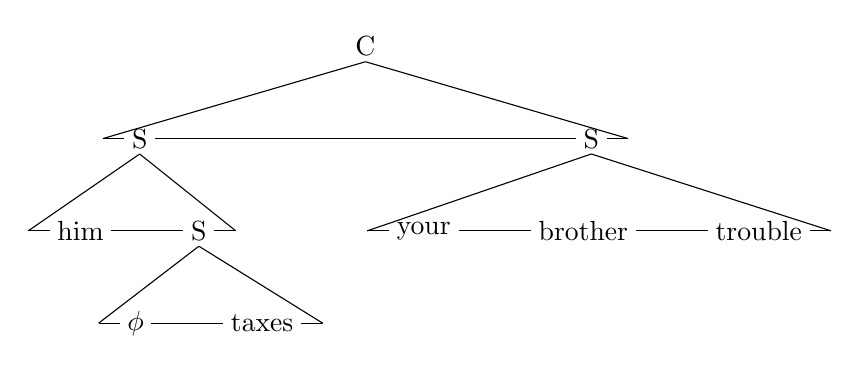
\begin{tikzpicture}
\node at (0.000000, 0.000000) {C};
\node at (-2.867583, -1.171530) {S};
\node at (-3.619319, -2.343060) {him};
\node at (-2.115846, -2.343060) {S};
\node at (-2.919325, -3.514590) {$\phi$};
\node at (-1.312366, -3.514590) {taxes};
\node at (2.867583, -1.171530) {S};
\node at (0.740266, -2.343060) {your};
\node at (2.767514, -2.343060) {brother};
\node at (4.994899, -2.343060) {trouble};
\draw (0.000000,-0.195255) -- (-3.336198,-1.171530);
\draw (0.000000,-0.195255) -- (3.336198,-1.171530);
\draw (-3.336198,-1.171530) -- (-3.065211,-1.171530);
\draw (-2.669955,-1.171530) -- (2.669955,-1.171530);
\draw (3.065211,-1.171530) -- (3.336198,-1.171530);
\draw (-2.867583,-1.366785) -- (-4.283191,-2.343060);
\draw (-2.867583,-1.366785) -- (-1.647231,-2.343060);
\draw (-4.283191,-2.343060) -- (-4.012204,-2.343060);
\draw (-3.226435,-2.343060) -- (-2.313474,-2.343060);
\draw (-1.918218,-2.343060) -- (-1.647231,-2.343060);
\draw (-2.115846,-2.538315) -- (-3.387940,-3.514590);
\draw (-2.115846,-2.538315) -- (-0.545010,-3.514590);
\draw (-3.387940,-3.514590) -- (-3.116953,-3.514590);
\draw (-2.721697,-3.514590) -- (-1.808736,-3.514590);
\draw (-0.815997,-3.514590) -- (-0.545010,-3.514590);
\draw (2.867583,-1.366785) -- (0.022211,-2.343060);
\draw (2.867583,-1.366785) -- (5.913091,-2.343060);
\draw (0.022211,-2.343060) -- (0.293199,-2.343060);
\draw (1.187334,-2.343060) -- (2.100296,-2.343060);
\draw (3.434732,-2.343060) -- (4.347694,-2.343060);
\draw (5.642104,-2.343060) -- (5.913091,-2.343060);
\end{tikzpicture}
}
\end{minipage}
\bigbreak

\clearpage

%%%%%%%%%%%%%%%%%%%%%%%%%%%%%%%%%%%%%%%%%%%%%%%%%%%%%%%%%%%%%%%%
%
%     (1.99) Anna's complaining about him infuriated Peter.
%
%%%%%%%%%%%%%%%%%%%%%%%%%%%%%%%%%%%%%%%%%%%%%%%%%%%%%%%%%%%%%%%%

\section*{(1.99) Anna's complaining about him infuriated Peter.}
\addcontentsline{toc}{section}{(1.99) Anna's complaining about him infuriated Peter.}

\bigbreak
\begin{enumerate*}
\item[(1.99)] Anna's complaining about him infuriated Peter.
\end{enumerate*}
\bigbreak
\bigbreak
\begin{minipage}{\textwidth}
\makebox[\textwidth][c]{
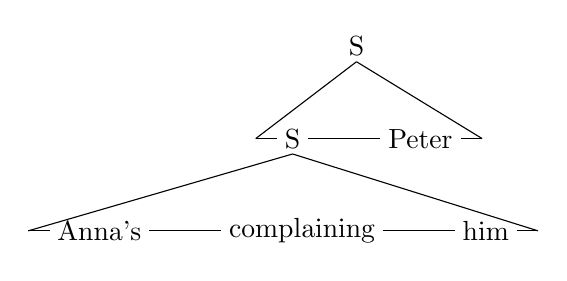
\begin{tikzpicture}
\node at (0.000000, 0.000000) {S};
\node at (-0.811778, -1.171530) {S};
\node at (-3.265172, -2.343060) {Anna's};
\node at (-0.691695, -2.343060) {complaining};
\node at (1.641617, -2.343060) {him};
\node at (0.811778, -1.171530) {Peter};
\draw (0.000000,-0.195255) -- (-1.280393,-1.171530);
\draw (0.000000,-0.195255) -- (1.595731,-1.171530);
\draw (-1.280393,-1.171530) -- (-1.009406,-1.171530);
\draw (-0.614150,-1.171530) -- (0.298812,-1.171530);
\draw (1.324743,-1.171530) -- (1.595731,-1.171530);
\draw (-0.811778,-1.366785) -- (-4.169208,-2.343060);
\draw (-0.811778,-1.366785) -- (2.305489,-2.343060);
\draw (-4.169208,-2.343060) -- (-3.898221,-2.343060);
\draw (-2.632123,-2.343060) -- (-1.719162,-2.343060);
\draw (0.335771,-2.343060) -- (1.248733,-2.343060);
\draw (2.034501,-2.343060) -- (2.305489,-2.343060);
\end{tikzpicture}
}
\end{minipage}
\bigbreak

\clearpage

%%%%%%%%%%%%%%%%%%%%%%%%%%%%%%%%%%%%%%%%%%%%%%%%%%%%%%%%%%%%%%%%
%
%     (1.100) The possibility that he will be unpopular doesn’t bother Fred.
%
%%%%%%%%%%%%%%%%%%%%%%%%%%%%%%%%%%%%%%%%%%%%%%%%%%%%%%%%%%%%%%%%

\section*{(1.100) The possibility that he will be unpopular doesn’t bother Fred.}
\addcontentsline{toc}{section}{(1.100) The possibility that he will be unpopular doesn’t bother Fred.}

\bigbreak
\begin{enumerate*}
\item[(1.100)] The possibility that he will be unpopular doesn’t bother Fred.
\end{enumerate*}
\bigbreak
\bigbreak
\begin{minipage}{\textwidth}
\makebox[\textwidth][c]{
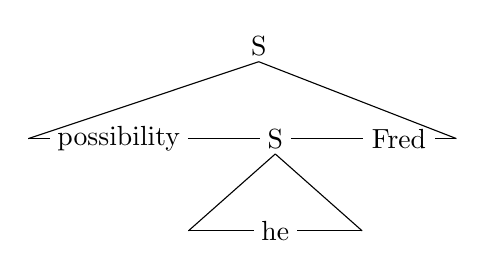
\begin{tikzpicture}
\node at (0.000000, 0.000000) {S};
\node at (-1.779273, -1.171530) {possibility};
\node at (0.209412, -1.171530) {S};
\node at (0.209412, -2.343060) {he};
\node at (1.779273, -1.171530) {Fred};
\draw (0.000000,-0.195255) -- (-2.928355,-1.171530);
\draw (0.000000,-0.195255) -- (2.509531,-1.171530);
\draw (-2.928355,-1.171530) -- (-2.657368,-1.171530);
\draw (-0.901177,-1.171530) -- (0.011784,-1.171530);
\draw (0.407040,-1.171530) -- (1.320002,-1.171530);
\draw (2.238543,-1.171530) -- (2.509531,-1.171530);
\draw (0.209412,-1.366785) -- (-0.893786,-2.343060);
\draw (0.209412,-1.366785) -- (1.312610,-2.343060);
\draw (-0.893786,-2.343060) -- (-0.066318,-2.343060);
\draw (0.485143,-2.343060) -- (1.312610,-2.343060);
\end{tikzpicture}
}
\end{minipage}
\bigbreak

\clearpage

%%%%%%%%%%%%%%%%%%%%%%%%%%%%%%%%%%%%%%%%%%%%%%%%%%%%%%%%%%%%%%%%
%
%     (1.101) John Adams was hungry after he woke up.
%
%%%%%%%%%%%%%%%%%%%%%%%%%%%%%%%%%%%%%%%%%%%%%%%%%%%%%%%%%%%%%%%%

\section*{(1.101) John Adams was hungry after he woke up.}
\addcontentsline{toc}{section}{(1.101) John Adams was hungry after he woke up.}

\bigbreak
\begin{enumerate*}
\item[(1.101)] John Adams was hungry after he woke up.
\end{enumerate*}
\bigbreak
\bigbreak
\begin{minipage}{\textwidth}
\makebox[\textwidth][c]{
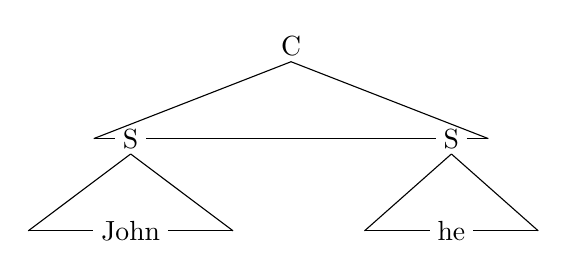
\begin{tikzpicture}
\node at (0.000000, 0.000000) {C};
\node at (-2.036768, -1.171530) {S};
\node at (-2.036768, -2.343060) {John};
\node at (2.036768, -1.171530) {S};
\node at (2.036768, -2.343060) {he};
\draw (0.000000,-0.195255) -- (-2.505383,-1.171530);
\draw (0.000000,-0.195255) -- (2.505383,-1.171530);
\draw (-2.505383,-1.171530) -- (-2.234396,-1.171530);
\draw (-1.839140,-1.171530) -- (1.839140,-1.171530);
\draw (2.234396,-1.171530) -- (2.505383,-1.171530);
\draw (-2.036768,-1.366785) -- (-3.337663,-2.343060);
\draw (-2.036768,-1.366785) -- (-0.735872,-2.343060);
\draw (-3.337663,-2.343060) -- (-2.510195,-2.343060);
\draw (-1.563340,-2.343060) -- (-0.735872,-2.343060);
\draw (2.036768,-1.366785) -- (0.933570,-2.343060);
\draw (2.036768,-1.366785) -- (3.139966,-2.343060);
\draw (0.933570,-2.343060) -- (1.761037,-2.343060);
\draw (2.312498,-2.343060) -- (3.139966,-2.343060);
\end{tikzpicture}
}
\end{minipage}
\bigbreak

\clearpage

%%%%%%%%%%%%%%%%%%%%%%%%%%%%%%%%%%%%%%%%%%%%%%%%%%%%%%%%%%%%%%%%
%
%     (1.102) Oscar wasn't disturbed that he was unpopular.
%
%%%%%%%%%%%%%%%%%%%%%%%%%%%%%%%%%%%%%%%%%%%%%%%%%%%%%%%%%%%%%%%%

\section*{(1.102) Oscar wasn't disturbed that he was unpopular.}
\addcontentsline{toc}{section}{(1.102) Oscar wasn't disturbed that he was unpopular.}

\bigbreak
\begin{enumerate*}
\item[(1.102)] Oscar wasn't disturbed that he was unpopular.
\end{enumerate*}
\bigbreak
\bigbreak
\begin{minipage}{\textwidth}
\makebox[\textwidth][c]{
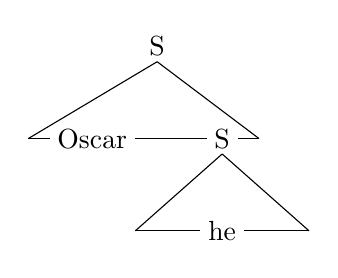
\begin{tikzpicture}
\node at (0.000000, 0.000000) {S};
\node at (-0.825690, -1.171530) {Oscar};
\node at (0.825690, -1.171530) {S};
\node at (0.825690, -2.343060) {he};
\draw (0.000000,-0.195255) -- (-1.637467,-1.171530);
\draw (0.000000,-0.195255) -- (1.294305,-1.171530);
\draw (-1.637467,-1.171530) -- (-1.366480,-1.171530);
\draw (-0.284900,-1.171530) -- (0.628062,-1.171530);
\draw (1.023318,-1.171530) -- (1.294305,-1.171530);
\draw (0.825690,-1.366785) -- (-0.277508,-2.343060);
\draw (0.825690,-1.366785) -- (1.928888,-2.343060);
\draw (-0.277508,-2.343060) -- (0.549960,-2.343060);
\draw (1.101420,-2.343060) -- (1.928888,-2.343060);
\end{tikzpicture}
}
\end{minipage}
\bigbreak

\clearpage

%%%%%%%%%%%%%%%%%%%%%%%%%%%%%%%%%%%%%%%%%%%%%%%%%%%%%%%%%%%%%%%%
%
%     (1.103) It would get your brother into trouble for him to refuse to pay taxes.
%
%%%%%%%%%%%%%%%%%%%%%%%%%%%%%%%%%%%%%%%%%%%%%%%%%%%%%%%%%%%%%%%%

\section*{(1.103) It would get your brother into trouble for him to refuse to pay taxes.}
\addcontentsline{toc}{section}{(1.103) It would get your brother into trouble for him to refuse to pay taxes.}

\bigbreak
\begin{enumerate*}
\item[(1.103)] It would get your brother into trouble for him to refuse to pay taxes.
\end{enumerate*}
\bigbreak
\bigbreak
\begin{minipage}{\textwidth}
\makebox[\textwidth][c]{
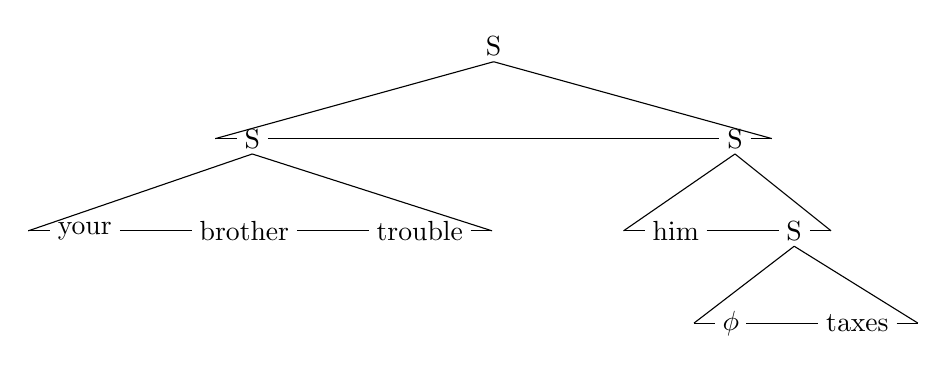
\begin{tikzpicture}
\node at (0.000000, 0.000000) {S};
\node at (-3.065279, -1.171530) {S};
\node at (-5.192595, -2.343060) {your};
\node at (-3.165348, -2.343060) {brother};
\node at (-0.937963, -2.343060) {trouble};
\node at (3.065279, -1.171530) {S};
\node at (2.313542, -2.343060) {him};
\node at (3.817016, -2.343060) {S};
\node at (3.013537, -3.514590) {$\phi$};
\node at (4.620496, -3.514590) {taxes};
\draw (0.000000,-0.195255) -- (-3.533894,-1.171530);
\draw (0.000000,-0.195255) -- (3.533894,-1.171530);
\draw (-3.533894,-1.171530) -- (-3.262907,-1.171530);
\draw (-2.867651,-1.171530) -- (2.867651,-1.171530);
\draw (3.262907,-1.171530) -- (3.533894,-1.171530);
\draw (-3.065279,-1.366785) -- (-5.910650,-2.343060);
\draw (-3.065279,-1.366785) -- (-0.019771,-2.343060);
\draw (-5.910650,-2.343060) -- (-5.639663,-2.343060);
\draw (-4.745528,-2.343060) -- (-3.832566,-2.343060);
\draw (-2.498129,-2.343060) -- (-1.585168,-2.343060);
\draw (-0.290758,-2.343060) -- (-0.019771,-2.343060);
\draw (3.065279,-1.366785) -- (1.649671,-2.343060);
\draw (3.065279,-1.366785) -- (4.285631,-2.343060);
\draw (1.649671,-2.343060) -- (1.920658,-2.343060);
\draw (2.706427,-2.343060) -- (3.619388,-2.343060);
\draw (4.014644,-2.343060) -- (4.285631,-2.343060);
\draw (3.817016,-2.538315) -- (2.544921,-3.514590);
\draw (3.817016,-2.538315) -- (5.387852,-3.514590);
\draw (2.544921,-3.514590) -- (2.815909,-3.514590);
\draw (3.211165,-3.514590) -- (4.124126,-3.514590);
\draw (5.116865,-3.514590) -- (5.387852,-3.514590);
\end{tikzpicture}
}
\end{minipage}
\bigbreak

\clearpage

%%%%%%%%%%%%%%%%%%%%%%%%%%%%%%%%%%%%%%%%%%%%%%%%%%%%%%%%%%%%%%%%
%
%     (1.104) Peter was infuriated at Anna's complaining about him.
%
%%%%%%%%%%%%%%%%%%%%%%%%%%%%%%%%%%%%%%%%%%%%%%%%%%%%%%%%%%%%%%%%

\section*{(1.104) Peter was infuriated at Anna's complaining about him.}
\addcontentsline{toc}{section}{(1.104) Peter was infuriated at Anna's complaining about him.}

\bigbreak
\begin{enumerate*}
\item[(1.104)] Peter was infuriated at Anna's complaining about him.
\end{enumerate*}
\bigbreak
\bigbreak
\begin{minipage}{\textwidth}
\makebox[\textwidth][c]{
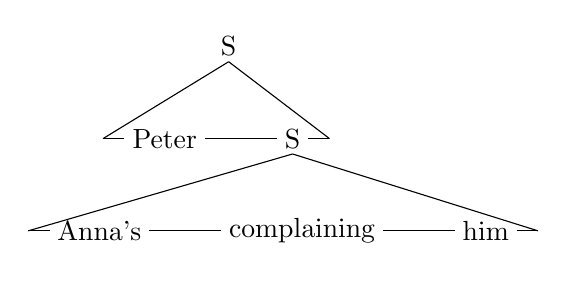
\begin{tikzpicture}
\node at (0.000000, 0.000000) {S};
\node at (-0.811778, -1.171530) {Peter};
\node at (0.811778, -1.171530) {S};
\node at (-1.641617, -2.343060) {Anna's};
\node at (0.931860, -2.343060) {complaining};
\node at (3.265172, -2.343060) {him};
\draw (0.000000,-0.195255) -- (-1.595731,-1.171530);
\draw (0.000000,-0.195255) -- (1.280393,-1.171530);
\draw (-1.595731,-1.171530) -- (-1.324743,-1.171530);
\draw (-0.298812,-1.171530) -- (0.614150,-1.171530);
\draw (1.009406,-1.171530) -- (1.280393,-1.171530);
\draw (0.811778,-1.366785) -- (-2.545653,-2.343060);
\draw (0.811778,-1.366785) -- (3.929044,-2.343060);
\draw (-2.545653,-2.343060) -- (-2.274666,-2.343060);
\draw (-1.008568,-2.343060) -- (-0.095607,-2.343060);
\draw (1.959327,-2.343060) -- (2.872288,-2.343060);
\draw (3.658057,-2.343060) -- (3.929044,-2.343060);
\end{tikzpicture}
}
\end{minipage}
\bigbreak

\clearpage

%%%%%%%%%%%%%%%%%%%%%%%%%%%%%%%%%%%%%%%%%%%%%%%%%%%%%%%%%%%%%%%%
%
%     (1.105) Fred isn't bothered by the possibility that he will be unpopular.
%
%%%%%%%%%%%%%%%%%%%%%%%%%%%%%%%%%%%%%%%%%%%%%%%%%%%%%%%%%%%%%%%%

\section*{(1.105) Fred isn't bothered by the possibility that he will be unpopular.}
\addcontentsline{toc}{section}{(1.105) Fred isn't bothered by the possibility that he will be unpopular.}

\bigbreak
\begin{enumerate*}
\item[(1.105)] Fred isn't bothered by the possibility that he will be unpopular.
\end{enumerate*}
\bigbreak
\bigbreak
\begin{minipage}{\textwidth}
\makebox[\textwidth][c]{
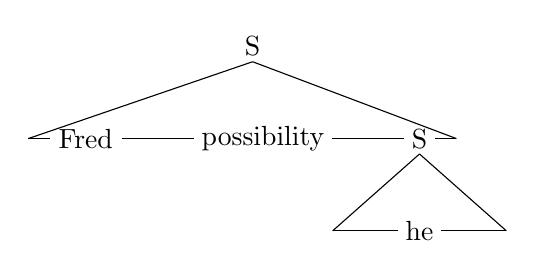
\begin{tikzpicture}
\node at (0.000000, 0.000000) {S};
\node at (-2.119506, -1.171530) {Fred};
\node at (0.130821, -1.171530) {possibility};
\node at (2.119506, -1.171530) {S};
\node at (2.119506, -2.343060) {he};
\draw (0.000000,-0.195255) -- (-2.849764,-1.171530);
\draw (0.000000,-0.195255) -- (2.588121,-1.171530);
\draw (-2.849764,-1.171530) -- (-2.578777,-1.171530);
\draw (-1.660235,-1.171530) -- (-0.747274,-1.171530);
\draw (1.008917,-1.171530) -- (1.921878,-1.171530);
\draw (2.317134,-1.171530) -- (2.588121,-1.171530);
\draw (2.119506,-1.366785) -- (1.016308,-2.343060);
\draw (2.119506,-1.366785) -- (3.222704,-2.343060);
\draw (1.016308,-2.343060) -- (1.843776,-2.343060);
\draw (2.395237,-2.343060) -- (3.222704,-2.343060);
\end{tikzpicture}
}
\end{minipage}
\bigbreak

\clearpage

%%%%%%%%%%%%%%%%%%%%%%%%%%%%%%%%%%%%%%%%%%%%%%%%%%%%%%%%%%%%%%%%
%
%     (1.106) *He was hungry after John Adams woke up.
%
%%%%%%%%%%%%%%%%%%%%%%%%%%%%%%%%%%%%%%%%%%%%%%%%%%%%%%%%%%%%%%%%

\section*{(1.106) *He was hungry after John Adams woke up.}
\addcontentsline{toc}{section}{(1.106) *He was hungry after John Adams woke up.}

\bigbreak
\begin{enumerate*}
\item[(1.106)] *He was hungry after John Adams woke up.
\end{enumerate*}
\bigbreak
\bigbreak
\begin{minipage}{\textwidth}
\makebox[\textwidth][c]{
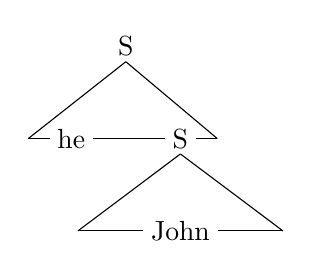
\begin{tikzpicture}
\node at (0.000000, 0.000000) {S};
\node at (-0.693160, -1.171530) {he};
\node at (0.693160, -1.171530) {S};
\node at (0.693160, -2.343060) {John};
\draw (0.000000,-0.195255) -- (-1.239877,-1.171530);
\draw (0.000000,-0.195255) -- (1.161775,-1.171530);
\draw (-1.239877,-1.171530) -- (-0.968890,-1.171530);
\draw (-0.417430,-1.171530) -- (0.495532,-1.171530);
\draw (0.890788,-1.171530) -- (1.161775,-1.171530);
\draw (0.693160,-1.366785) -- (-0.607735,-2.343060);
\draw (0.693160,-1.366785) -- (1.994055,-2.343060);
\draw (-0.607735,-2.343060) -- (0.219732,-2.343060);
\draw (1.166587,-2.343060) -- (1.994055,-2.343060);
\end{tikzpicture}
}
\end{minipage}
\bigbreak

\clearpage

%%%%%%%%%%%%%%%%%%%%%%%%%%%%%%%%%%%%%%%%%%%%%%%%%%%%%%%%%%%%%%%%
%
%     (1.107) *He wasn't disturbed that Oscar was unpopular.
%
%%%%%%%%%%%%%%%%%%%%%%%%%%%%%%%%%%%%%%%%%%%%%%%%%%%%%%%%%%%%%%%%

\section*{(1.107) *He wasn't disturbed that Oscar was unpopular.}
\addcontentsline{toc}{section}{(1.107) *He wasn't disturbed that Oscar was unpopular.}

\bigbreak
\begin{enumerate*}
\item[(1.107)] *He wasn't disturbed that Oscar was unpopular.
\end{enumerate*}
\bigbreak
\bigbreak
\begin{minipage}{\textwidth}
\makebox[\textwidth][c]{
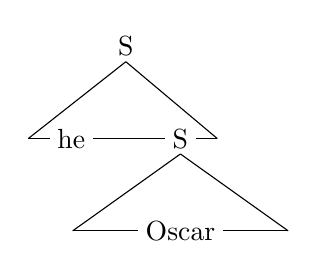
\begin{tikzpicture}
\node at (0.000000, 0.000000) {S};
\node at (-0.693160, -1.171530) {he};
\node at (0.693160, -1.171530) {S};
\node at (0.693160, -2.343060) {Oscar};
\draw (0.000000,-0.195255) -- (-1.239877,-1.171530);
\draw (0.000000,-0.195255) -- (1.161775,-1.171530);
\draw (-1.239877,-1.171530) -- (-0.968890,-1.171530);
\draw (-0.417430,-1.171530) -- (0.495532,-1.171530);
\draw (0.890788,-1.171530) -- (1.161775,-1.171530);
\draw (0.693160,-1.366785) -- (-0.675098,-2.343060);
\draw (0.693160,-1.366785) -- (2.061418,-2.343060);
\draw (-0.675098,-2.343060) -- (0.152370,-2.343060);
\draw (1.233950,-2.343060) -- (2.061418,-2.343060);
\end{tikzpicture}
}
\end{minipage}
\bigbreak

\clearpage

%%%%%%%%%%%%%%%%%%%%%%%%%%%%%%%%%%%%%%%%%%%%%%%%%%%%%%%%%%%%%%%%
%
%     (1.108) *It would get him into trouble for your brother to refuse to pay taxes.
%
%%%%%%%%%%%%%%%%%%%%%%%%%%%%%%%%%%%%%%%%%%%%%%%%%%%%%%%%%%%%%%%%

\section*{(1.108) *It would get him into trouble for your brother to refuse to pay taxes.}
\addcontentsline{toc}{section}{(1.108) *It would get him into trouble for your brother to refuse to pay taxes.}

\bigbreak
\begin{enumerate*}
\item[(1.108)] *It would get him into trouble for your brother to refuse to pay taxes.
\end{enumerate*}
\bigbreak
\bigbreak
\begin{minipage}{\textwidth}
\makebox[\textwidth][c]{
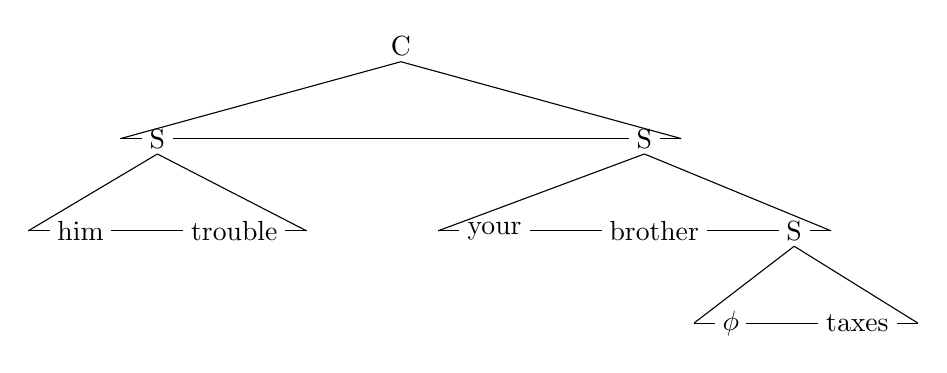
\begin{tikzpicture}
\node at (0.000000, 0.000000) {C};
\node at (-3.092371, -1.171530) {S};
\node at (-4.068896, -2.343060) {him};
\node at (-2.115846, -2.343060) {trouble};
\node at (3.092371, -1.171530) {S};
\node at (1.189843, -2.343060) {your};
\node at (3.217091, -2.343060) {brother};
\node at (4.994899, -2.343060) {S};
\node at (4.191419, -3.514590) {$\phi$};
\node at (5.798378, -3.514590) {taxes};
\draw (0.000000,-0.195255) -- (-3.560986,-1.171530);
\draw (0.000000,-0.195255) -- (3.560986,-1.171530);
\draw (-3.560986,-1.171530) -- (-3.289999,-1.171530);
\draw (-2.894743,-1.171530) -- (2.894743,-1.171530);
\draw (3.289999,-1.171530) -- (3.560986,-1.171530);
\draw (-3.092371,-1.366785) -- (-4.732768,-2.343060);
\draw (-3.092371,-1.366785) -- (-1.197654,-2.343060);
\draw (-4.732768,-2.343060) -- (-4.461781,-2.343060);
\draw (-3.676012,-2.343060) -- (-2.763051,-2.343060);
\draw (-1.468641,-2.343060) -- (-1.197654,-2.343060);
\draw (3.092371,-1.366785) -- (0.471788,-2.343060);
\draw (3.092371,-1.366785) -- (5.463514,-2.343060);
\draw (0.471788,-2.343060) -- (0.742775,-2.343060);
\draw (1.636911,-2.343060) -- (2.549872,-2.343060);
\draw (3.884309,-2.343060) -- (4.797271,-2.343060);
\draw (5.192527,-2.343060) -- (5.463514,-2.343060);
\draw (4.994899,-2.538315) -- (3.722804,-3.514590);
\draw (4.994899,-2.538315) -- (6.565735,-3.514590);
\draw (3.722804,-3.514590) -- (3.993791,-3.514590);
\draw (4.389047,-3.514590) -- (5.302009,-3.514590);
\draw (6.294748,-3.514590) -- (6.565735,-3.514590);
\end{tikzpicture}
}
\end{minipage}
\bigbreak

\clearpage

%%%%%%%%%%%%%%%%%%%%%%%%%%%%%%%%%%%%%%%%%%%%%%%%%%%%%%%%%%%%%%%%
%
%     (1.109) *He was infuriated at Anna's complaining about Peter.
%
%%%%%%%%%%%%%%%%%%%%%%%%%%%%%%%%%%%%%%%%%%%%%%%%%%%%%%%%%%%%%%%%

\section*{(1.109) *He was infuriated at Anna's complaining about Peter.}
\addcontentsline{toc}{section}{(1.109) *He was infuriated at Anna's complaining about Peter.}

\bigbreak
\begin{enumerate*}
\item[(1.109)] *He was infuriated at Anna's complaining about Peter.
\end{enumerate*}
\bigbreak
\bigbreak
\begin{minipage}{\textwidth}
\makebox[\textwidth][c]{
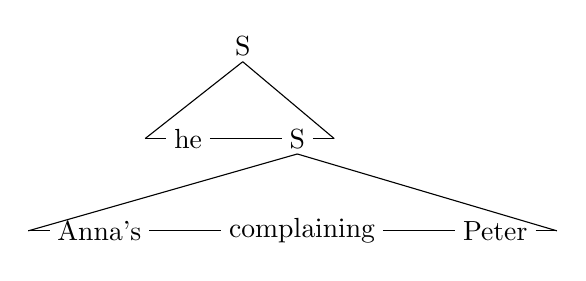
\begin{tikzpicture}
\node at (0.000000, 0.000000) {S};
\node at (-0.693160, -1.171530) {he};
\node at (0.693160, -1.171530) {S};
\node at (-1.820276, -2.343060) {Anna's};
\node at (0.753201, -2.343060) {complaining};
\node at (3.206595, -2.343060) {Peter};
\draw (0.000000,-0.195255) -- (-1.239877,-1.171530);
\draw (0.000000,-0.195255) -- (1.161775,-1.171530);
\draw (-1.239877,-1.171530) -- (-0.968890,-1.171530);
\draw (-0.417430,-1.171530) -- (0.495532,-1.171530);
\draw (0.890788,-1.171530) -- (1.161775,-1.171530);
\draw (0.693160,-1.366785) -- (-2.724312,-2.343060);
\draw (0.693160,-1.366785) -- (3.990548,-2.343060);
\draw (-2.724312,-2.343060) -- (-2.453325,-2.343060);
\draw (-1.187227,-2.343060) -- (-0.274265,-2.343060);
\draw (1.780668,-2.343060) -- (2.693629,-2.343060);
\draw (3.719561,-2.343060) -- (3.990548,-2.343060);
\end{tikzpicture}
}
\end{minipage}
\bigbreak

\clearpage

%%%%%%%%%%%%%%%%%%%%%%%%%%%%%%%%%%%%%%%%%%%%%%%%%%%%%%%%%%%%%%%%
%
%     (1.110) *He isn't bothered by the possibility that Fred will be unpopular.
%
%%%%%%%%%%%%%%%%%%%%%%%%%%%%%%%%%%%%%%%%%%%%%%%%%%%%%%%%%%%%%%%%

\section*{(1.110) *He isn't bothered by the possibility that Fred will be unpopular.}
\addcontentsline{toc}{section}{(1.110) *He isn't bothered by the possibility that Fred will be unpopular.}

\bigbreak
\begin{enumerate*}
\item[(1.110)] *He isn't bothered by the possibility that Fred will be unpopular.
\end{enumerate*}
\bigbreak
\bigbreak
\begin{minipage}{\textwidth}
\makebox[\textwidth][c]{
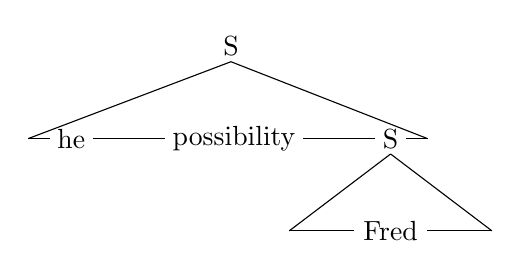
\begin{tikzpicture}
\node at (0.000000, 0.000000) {S};
\node at (-2.027736, -1.171530) {he};
\node at (0.039051, -1.171530) {possibility};
\node at (2.027736, -1.171530) {S};
\node at (2.027736, -2.343060) {Fred};
\draw (0.000000,-0.195255) -- (-2.574453,-1.171530);
\draw (0.000000,-0.195255) -- (2.496351,-1.171530);
\draw (-2.574453,-1.171530) -- (-2.303466,-1.171530);
\draw (-1.752006,-1.171530) -- (-0.839044,-1.171530);
\draw (0.917147,-1.171530) -- (1.830108,-1.171530);
\draw (2.225364,-1.171530) -- (2.496351,-1.171530);
\draw (2.027736,-1.366785) -- (0.740997,-2.343060);
\draw (2.027736,-1.366785) -- (3.314475,-2.343060);
\draw (0.740997,-2.343060) -- (1.568465,-2.343060);
\draw (2.487007,-2.343060) -- (3.314475,-2.343060);
\end{tikzpicture}
}
\end{minipage}
\bigbreak

\clearpage

%%%%%%%%%%%%%%%%%%%%%%%%%%%%%%%%%%%%%%%%%%%%%%%%%%%%%%%%%%%%%%%%
%
%     (1.111) Penelope cursed Peter and slandered him.
%
%%%%%%%%%%%%%%%%%%%%%%%%%%%%%%%%%%%%%%%%%%%%%%%%%%%%%%%%%%%%%%%%

\section*{(1.111) Penelope cursed Peter and slandered him.}
\addcontentsline{toc}{section}{(1.111) Penelope cursed Peter and slandered him.}

\bigbreak
\begin{enumerate*}
\item[(1.111)] Penelope cursed Peter and slandered him.
\end{enumerate*}
\bigbreak
\bigbreak
\begin{minipage}{\textwidth}
\makebox[\textwidth][c]{
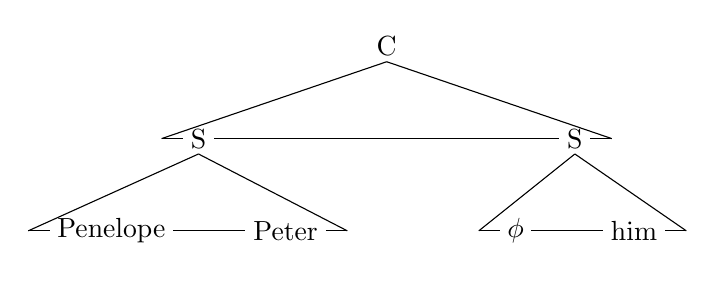
\begin{tikzpicture}
\node at (0.000000, 0.000000) {C};
\node at (-2.389814, -1.171530) {S};
\node at (-3.495696, -2.343060) {Penelope};
\node at (-1.283933, -2.343060) {Peter};
\node at (2.389814, -1.171530) {S};
\node at (1.638078, -2.343060) {$\phi$};
\node at (3.141551, -2.343060) {him};
\draw (0.000000,-0.195255) -- (-2.858429,-1.171530);
\draw (0.000000,-0.195255) -- (2.858429,-1.171530);
\draw (-2.858429,-1.171530) -- (-2.587442,-1.171530);
\draw (-2.192186,-1.171530) -- (2.192186,-1.171530);
\draw (2.587442,-1.171530) -- (2.858429,-1.171530);
\draw (-2.389814,-1.366785) -- (-4.552519,-2.343060);
\draw (-2.389814,-1.366785) -- (-0.499980,-2.343060);
\draw (-4.552519,-2.343060) -- (-4.281532,-2.343060);
\draw (-2.709860,-2.343060) -- (-1.796898,-2.343060);
\draw (-0.770967,-2.343060) -- (-0.499980,-2.343060);
\draw (2.389814,-1.366785) -- (1.169462,-2.343060);
\draw (2.389814,-1.366785) -- (3.805423,-2.343060);
\draw (1.169462,-2.343060) -- (1.440449,-2.343060);
\draw (1.835706,-2.343060) -- (2.748667,-2.343060);
\draw (3.534435,-2.343060) -- (3.805423,-2.343060);
\end{tikzpicture}
}
\end{minipage}
\bigbreak

\clearpage

%%%%%%%%%%%%%%%%%%%%%%%%%%%%%%%%%%%%%%%%%%%%%%%%%%%%%%%%%%%%%%%%
%
%     (1.112) *Penelope cursed him and slandered Peter.
%
%%%%%%%%%%%%%%%%%%%%%%%%%%%%%%%%%%%%%%%%%%%%%%%%%%%%%%%%%%%%%%%%

\section*{(1.112) *Penelope cursed him and slandered Peter.}
\addcontentsline{toc}{section}{(1.112) *Penelope cursed him and slandered Peter.}

\bigbreak
\begin{enumerate*}
\item[(1.112)] *Penelope cursed him and slandered Peter.
\end{enumerate*}
\bigbreak
\bigbreak
\begin{minipage}{\textwidth}
\makebox[\textwidth][c]{
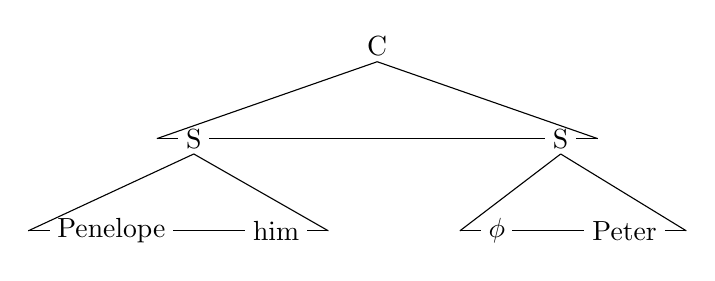
\begin{tikzpicture}
\node at (0.000000, 0.000000) {C};
\node at (-2.329774, -1.171530) {S};
\node at (-3.375614, -2.343060) {Penelope};
\node at (-1.283933, -2.343060) {him};
\node at (2.329774, -1.171530) {S};
\node at (1.517996, -2.343060) {$\phi$};
\node at (3.141551, -2.343060) {Peter};
\draw (0.000000,-0.195255) -- (-2.798389,-1.171530);
\draw (0.000000,-0.195255) -- (2.798389,-1.171530);
\draw (-2.798389,-1.171530) -- (-2.527402,-1.171530);
\draw (-2.132146,-1.171530) -- (2.132146,-1.171530);
\draw (2.527402,-1.171530) -- (2.798389,-1.171530);
\draw (-2.329774,-1.366785) -- (-4.432438,-2.343060);
\draw (-2.329774,-1.366785) -- (-0.620061,-2.343060);
\draw (-4.432438,-2.343060) -- (-4.161451,-2.343060);
\draw (-2.589778,-2.343060) -- (-1.676817,-2.343060);
\draw (-0.891048,-2.343060) -- (-0.620061,-2.343060);
\draw (2.329774,-1.366785) -- (1.049381,-2.343060);
\draw (2.329774,-1.366785) -- (3.925504,-2.343060);
\draw (1.049381,-2.343060) -- (1.320368,-2.343060);
\draw (1.715624,-2.343060) -- (2.628585,-2.343060);
\draw (3.654517,-2.343060) -- (3.925504,-2.343060);
\end{tikzpicture}
}
\end{minipage}
\bigbreak

\clearpage

%%%%%%%%%%%%%%%%%%%%%%%%%%%%%%%%%%%%%%%%%%%%%%%%%%%%%%%%%%%%%%%%
%
%     (1.113) The interest in visiting Las Vegas that Mary displayed is typical of gamblers.
%
%%%%%%%%%%%%%%%%%%%%%%%%%%%%%%%%%%%%%%%%%%%%%%%%%%%%%%%%%%%%%%%%

\section*{(1.113) The interest in visiting Las Vegas that Mary displayed is typical of gamblers.}
\addcontentsline{toc}{section}{(1.113) The interest in visiting Las Vegas that Mary displayed is typical of gamblers.}

\bigbreak
\begin{enumerate*}
\item[(1.113)] The interest in visiting Las Vegas that Mary displayed is typical of gamblers.
\end{enumerate*}
\bigbreak
\bigbreak
\begin{minipage}{\textwidth}
\makebox[\textwidth][c]{
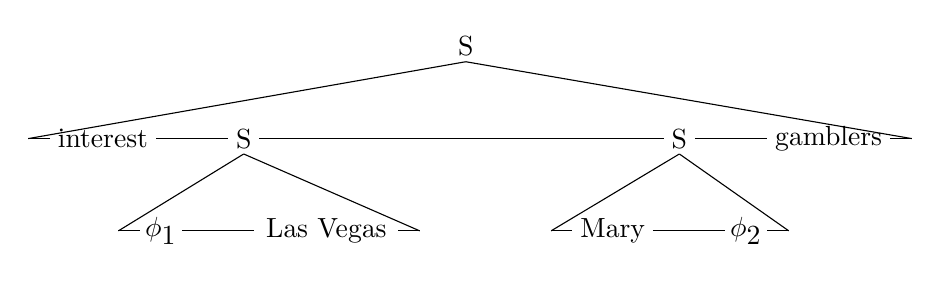
\begin{tikzpicture}
\node at (0.000000, 0.000000) {S};
\node at (-4.608291, -1.171530) {interest};
\node at (-2.820233, -1.171530) {S};
\node at (-3.869491, -2.343060) {${\phi_{\textrm{1}}}$};
\node at (-1.770975, -2.343060) {Las Vegas};
\node at (2.712841, -1.171530) {S};
\node at (1.865673, -2.343060) {Mary};
\node at (3.560010, -2.343060) {${\phi_{\textrm{2}}}$};
\node at (4.608291, -1.171530) {gamblers};
\draw (0.000000,-0.195255) -- (-5.556747,-1.171530);
\draw (0.000000,-0.195255) -- (5.664139,-1.171530);
\draw (-5.556747,-1.171530) -- (-5.285760,-1.171530);
\draw (-3.930822,-1.171530) -- (-3.017861,-1.171530);
\draw (-2.622605,-1.171530) -- (2.515213,-1.171530);
\draw (2.910470,-1.171530) -- (3.823431,-1.171530);
\draw (5.393152,-1.171530) -- (5.664139,-1.171530);
\draw (-2.820233,-1.366785) -- (-4.411327,-2.343060);
\draw (-2.820233,-1.366785) -- (-0.585282,-2.343060);
\draw (-4.411327,-2.343060) -- (-4.140340,-2.343060);
\draw (-3.598642,-2.343060) -- (-2.685681,-2.343060);
\draw (-0.856269,-2.343060) -- (-0.585282,-2.343060);
\draw (2.712841,-1.366785) -- (1.084160,-2.343060);
\draw (2.712841,-1.366785) -- (4.101846,-2.343060);
\draw (1.084160,-2.343060) -- (1.355147,-2.343060);
\draw (2.376199,-2.343060) -- (3.289161,-2.343060);
\draw (3.830859,-2.343060) -- (4.101846,-2.343060);
\end{tikzpicture}
}
\end{minipage}
\bigbreak

\clearpage

%%%%%%%%%%%%%%%%%%%%%%%%%%%%%%%%%%%%%%%%%%%%%%%%%%%%%%%%%%%%%%%%
%
%     (5.2) June hates flowers, but she waters them anyway.
%
%%%%%%%%%%%%%%%%%%%%%%%%%%%%%%%%%%%%%%%%%%%%%%%%%%%%%%%%%%%%%%%%

\section*{(5.2) June hates flowers, but she waters them anyway.}
\addcontentsline{toc}{section}{(5.2) June hates flowers, but she waters them anyway.}

\bigbreak
\begin{enumerate*}
\item[(5.2)] June hates flowers, but she waters them anyway.
\end{enumerate*}
\bigbreak
\bigbreak
\begin{minipage}{\textwidth}
\makebox[\textwidth][c]{
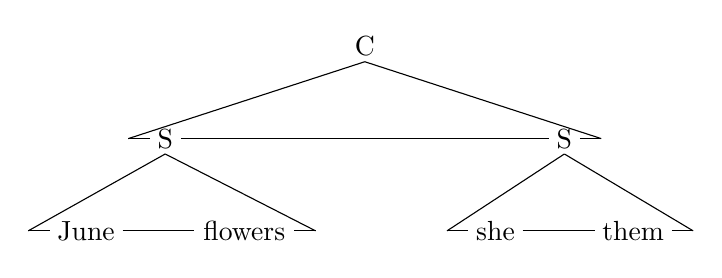
\begin{tikzpicture}
\node at (0.000000, 0.000000) {C};
\node at (-2.534670, -1.171530) {S};
\node at (-3.539751, -2.343060) {June};
\node at (-1.529589, -2.343060) {flowers};
\node at (2.534670, -1.171530) {S};
\node at (1.660410, -2.343060) {she};
\node at (3.408929, -2.343060) {them};
\draw (0.000000,-0.195255) -- (-3.003285,-1.171530);
\draw (0.000000,-0.195255) -- (3.003285,-1.171530);
\draw (-3.003285,-1.171530) -- (-2.732298,-1.171530);
\draw (-2.337042,-1.171530) -- (2.337042,-1.171530);
\draw (2.732298,-1.171530) -- (3.003285,-1.171530);
\draw (-2.534670,-1.366785) -- (-4.274402,-2.343060);
\draw (-2.534670,-1.366785) -- (-0.625065,-2.343060);
\draw (-4.274402,-2.343060) -- (-4.003415,-2.343060);
\draw (-3.076087,-2.343060) -- (-2.163125,-2.343060);
\draw (-0.896052,-2.343060) -- (-0.625065,-2.343060);
\draw (2.534670,-1.366785) -- (1.044377,-2.343060);
\draw (2.534670,-1.366785) -- (4.170428,-2.343060);
\draw (1.044377,-2.343060) -- (1.315364,-2.343060);
\draw (2.005456,-2.343060) -- (2.918417,-2.343060);
\draw (3.899441,-2.343060) -- (4.170428,-2.343060);
\end{tikzpicture}
}
\end{minipage}
\bigbreak

\clearpage

%%%%%%%%%%%%%%%%%%%%%%%%%%%%%%%%%%%%%%%%%%%%%%%%%%%%%%%%%%%%%%%%
%
%     (8.1) John wants to give June a present, but he isn't sure she’ll like it.
%
%%%%%%%%%%%%%%%%%%%%%%%%%%%%%%%%%%%%%%%%%%%%%%%%%%%%%%%%%%%%%%%%

\section*{(8.1) John wants to give June a present, but he isn't sure she’ll like it.}
\addcontentsline{toc}{section}{(8.1) John wants to give June a present, but he isn't sure she’ll like it.}

\bigbreak
\begin{enumerate*}
\item[(8.1)] John wants to give June a present, but he isn't sure she’ll like it.
\end{enumerate*}
\bigbreak
\bigbreak
\begin{minipage}{\textwidth}
\makebox[\textwidth][c]{
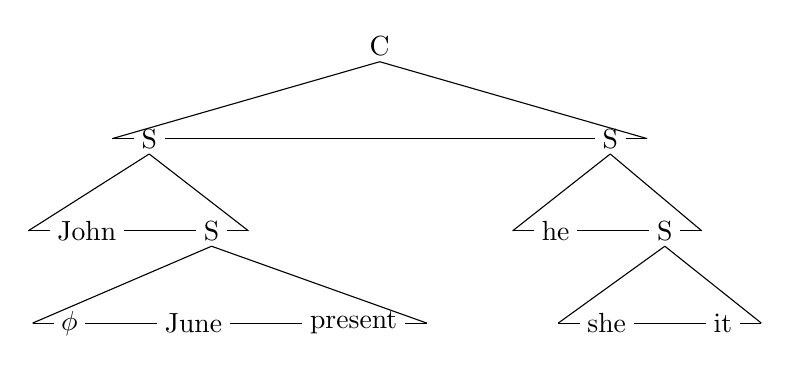
\begin{tikzpicture}
\node at (0.000000, 0.000000) {C};
\node at (-2.927623, -1.171530) {S};
\node at (-3.719631, -2.343060) {John};
\node at (-2.135614, -2.343060) {S};
\node at (-3.940026, -3.514590) {$\phi$};
\node at (-2.365772, -3.514590) {June};
\node at (-0.331203, -3.514590) {present};
\node at (2.927623, -1.171530) {S};
\node at (2.234463, -2.343060) {he};
\node at (3.620783, -2.343060) {S};
\node at (2.883202, -3.514590) {she};
\node at (4.358363, -3.514590) {it};
\draw (0.000000,-0.195255) -- (-3.396238,-1.171530);
\draw (0.000000,-0.195255) -- (3.396238,-1.171530);
\draw (-3.396238,-1.171530) -- (-3.125251,-1.171530);
\draw (-2.729995,-1.171530) -- (2.729995,-1.171530);
\draw (3.125251,-1.171530) -- (3.396238,-1.171530);
\draw (-2.927623,-1.366785) -- (-4.464046,-2.343060);
\draw (-2.927623,-1.366785) -- (-1.666999,-2.343060);
\draw (-4.464046,-2.343060) -- (-4.193058,-2.343060);
\draw (-3.246204,-2.343060) -- (-2.333242,-2.343060);
\draw (-1.937986,-2.343060) -- (-1.666999,-2.343060);
\draw (-2.135614,-2.538315) -- (-4.408641,-3.514590);
\draw (-2.135614,-2.538315) -- (0.597727,-3.514590);
\draw (-4.408641,-3.514590) -- (-4.137654,-3.514590);
\draw (-3.742397,-3.514590) -- (-2.829436,-3.514590);
\draw (-1.902108,-3.514590) -- (-0.989147,-3.514590);
\draw (0.326740,-3.514590) -- (0.597727,-3.514590);
\draw (2.927623,-1.366785) -- (1.687746,-2.343060);
\draw (2.927623,-1.366785) -- (4.089398,-2.343060);
\draw (1.687746,-2.343060) -- (1.958733,-2.343060);
\draw (2.510193,-2.343060) -- (3.423154,-2.343060);
\draw (3.818411,-2.343060) -- (4.089398,-2.343060);
\draw (3.620783,-2.538315) -- (2.267169,-3.514590);
\draw (3.620783,-2.538315) -- (4.846504,-3.514590);
\draw (2.267169,-3.514590) -- (2.538156,-3.514590);
\draw (3.228248,-3.514590) -- (4.141209,-3.514590);
\draw (4.575517,-3.514590) -- (4.846504,-3.514590);
\end{tikzpicture}
}
\end{minipage}
\bigbreak

\clearpage

%%%%%%%%%%%%%%%%%%%%%%%%%%%%%%%%%%%%%%%%%%%%%%%%%%%%%%%%%%%%%%%%
%
%     (10.1) John wants to give June a present, but he isn't sure she’ll like it.
%
%%%%%%%%%%%%%%%%%%%%%%%%%%%%%%%%%%%%%%%%%%%%%%%%%%%%%%%%%%%%%%%%

\section*{(10.1) John wants to give June a present, but he isn't sure she’ll like it.}
\addcontentsline{toc}{section}{(10.1) John wants to give June a present, but he isn't sure she’ll like it.}

\bigbreak
\begin{enumerate*}
\item[(10.1)] John wants to give June a present, but he isn't sure she’ll like it.
\end{enumerate*}
\bigbreak
\bigbreak
\begin{minipage}{\textwidth}
\makebox[\textwidth][c]{
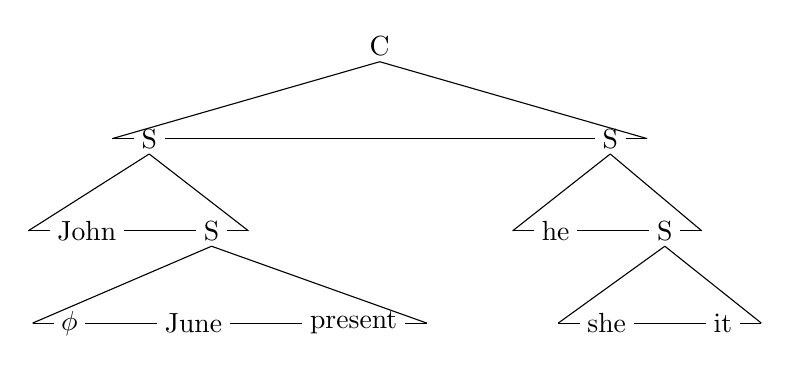
\begin{tikzpicture}
\node at (0.000000, 0.000000) {C};
\node at (-2.927623, -1.171530) {S};
\node at (-3.719631, -2.343060) {John};
\node at (-2.135614, -2.343060) {S};
\node at (-3.940026, -3.514590) {$\phi$};
\node at (-2.365772, -3.514590) {June};
\node at (-0.331203, -3.514590) {present};
\node at (2.927623, -1.171530) {S};
\node at (2.234463, -2.343060) {he};
\node at (3.620783, -2.343060) {S};
\node at (2.883202, -3.514590) {she};
\node at (4.358363, -3.514590) {it};
\draw (0.000000,-0.195255) -- (-3.396238,-1.171530);
\draw (0.000000,-0.195255) -- (3.396238,-1.171530);
\draw (-3.396238,-1.171530) -- (-3.125251,-1.171530);
\draw (-2.729995,-1.171530) -- (2.729995,-1.171530);
\draw (3.125251,-1.171530) -- (3.396238,-1.171530);
\draw (-2.927623,-1.366785) -- (-4.464046,-2.343060);
\draw (-2.927623,-1.366785) -- (-1.666999,-2.343060);
\draw (-4.464046,-2.343060) -- (-4.193058,-2.343060);
\draw (-3.246204,-2.343060) -- (-2.333242,-2.343060);
\draw (-1.937986,-2.343060) -- (-1.666999,-2.343060);
\draw (-2.135614,-2.538315) -- (-4.408641,-3.514590);
\draw (-2.135614,-2.538315) -- (0.597727,-3.514590);
\draw (-4.408641,-3.514590) -- (-4.137654,-3.514590);
\draw (-3.742397,-3.514590) -- (-2.829436,-3.514590);
\draw (-1.902108,-3.514590) -- (-0.989147,-3.514590);
\draw (0.326740,-3.514590) -- (0.597727,-3.514590);
\draw (2.927623,-1.366785) -- (1.687746,-2.343060);
\draw (2.927623,-1.366785) -- (4.089398,-2.343060);
\draw (1.687746,-2.343060) -- (1.958733,-2.343060);
\draw (2.510193,-2.343060) -- (3.423154,-2.343060);
\draw (3.818411,-2.343060) -- (4.089398,-2.343060);
\draw (3.620783,-2.538315) -- (2.267169,-3.514590);
\draw (3.620783,-2.538315) -- (4.846504,-3.514590);
\draw (2.267169,-3.514590) -- (2.538156,-3.514590);
\draw (3.228248,-3.514590) -- (4.141209,-3.514590);
\draw (4.575517,-3.514590) -- (4.846504,-3.514590);
\end{tikzpicture}
}
\end{minipage}
\bigbreak

\clearpage

%%%%%%%%%%%%%%%%%%%%%%%%%%%%%%%%%%%%%%%%%%%%%%%%%%%%%%%%%%%%%%%%
%
%     (10.2) Janet saw herself.
%
%%%%%%%%%%%%%%%%%%%%%%%%%%%%%%%%%%%%%%%%%%%%%%%%%%%%%%%%%%%%%%%%

\section*{(10.2) Janet saw herself.}
\addcontentsline{toc}{section}{(10.2) Janet saw herself.}

\bigbreak
\begin{enumerate*}
\item[(10.2)] Janet saw herself.
\end{enumerate*}
\bigbreak
\bigbreak
\begin{minipage}{\textwidth}
\makebox[\textwidth][c]{
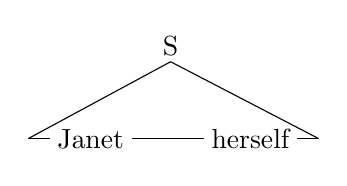
\begin{tikzpicture}
\node at (0.000000, 0.000000) {S};
\node at (-1.014844, -1.171530) {Janet};
\node at (1.014844, -1.171530) {herself};
\draw (0.000000,-0.195255) -- (-1.808072,-1.171530);
\draw (0.000000,-0.195255) -- (1.880316,-1.171530);
\draw (-1.808072,-1.171530) -- (-1.537085,-1.171530);
\draw (-0.492603,-1.171530) -- (0.420359,-1.171530);
\draw (1.609329,-1.171530) -- (1.880316,-1.171530);
\end{tikzpicture}
}
\end{minipage}
\bigbreak

\clearpage

%%%%%%%%%%%%%%%%%%%%%%%%%%%%%%%%%%%%%%%%%%%%%%%%%%%%%%%%%%%%%%%%
%
%     (10.3) Janet saw her.
%
%%%%%%%%%%%%%%%%%%%%%%%%%%%%%%%%%%%%%%%%%%%%%%%%%%%%%%%%%%%%%%%%

\section*{(10.3) Janet saw her.}
\addcontentsline{toc}{section}{(10.3) Janet saw her.}

\bigbreak
\begin{enumerate*}
\item[(10.3)] Janet saw her.
\end{enumerate*}
\bigbreak
\bigbreak
\begin{minipage}{\textwidth}
\makebox[\textwidth][c]{
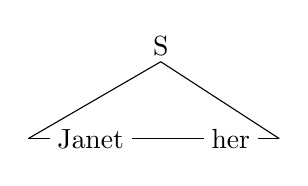
\begin{tikzpicture}
\node at (0.000000, 0.000000) {S};
\node at (-0.889880, -1.171530) {Janet};
\node at (0.889880, -1.171530) {her};
\draw (0.000000,-0.195255) -- (-1.683108,-1.171530);
\draw (0.000000,-0.195255) -- (1.505425,-1.171530);
\draw (-1.683108,-1.171530) -- (-1.412121,-1.171530);
\draw (-0.367639,-1.171530) -- (0.545322,-1.171530);
\draw (1.234438,-1.171530) -- (1.505425,-1.171530);
\end{tikzpicture}
}
\end{minipage}
\bigbreak

\clearpage

%%%%%%%%%%%%%%%%%%%%%%%%%%%%%%%%%%%%%%%%%%%%%%%%%%%%%%%%%%%%%%%%
%
%     (10.4) *Janet saw himself.
%
%%%%%%%%%%%%%%%%%%%%%%%%%%%%%%%%%%%%%%%%%%%%%%%%%%%%%%%%%%%%%%%%

\section*{(10.4) *Janet saw himself.}
\addcontentsline{toc}{section}{(10.4) *Janet saw himself.}

\bigbreak
\begin{enumerate*}
\item[(10.4)] *Janet saw himself.
\end{enumerate*}
\bigbreak
\bigbreak
\begin{minipage}{\textwidth}
\makebox[\textwidth][c]{
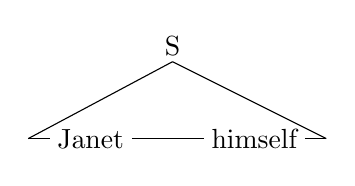
\begin{tikzpicture}
\node at (0.000000, 0.000000) {S};
\node at (-1.039007, -1.171530) {Janet};
\node at (1.039007, -1.171530) {himself};
\draw (0.000000,-0.195255) -- (-1.832235,-1.171530);
\draw (0.000000,-0.195255) -- (1.952806,-1.171530);
\draw (-1.832235,-1.171530) -- (-1.561248,-1.171530);
\draw (-0.516766,-1.171530) -- (0.396195,-1.171530);
\draw (1.681819,-1.171530) -- (1.952806,-1.171530);
\end{tikzpicture}
}
\end{minipage}
\bigbreak

\clearpage

%%%%%%%%%%%%%%%%%%%%%%%%%%%%%%%%%%%%%%%%%%%%%%%%%%%%%%%%%%%%%%%%
%
%     (10.5) The men threw a smokescreen around themselves.
%
%%%%%%%%%%%%%%%%%%%%%%%%%%%%%%%%%%%%%%%%%%%%%%%%%%%%%%%%%%%%%%%%

\section*{(10.5) The men threw a smokescreen around themselves.}
\addcontentsline{toc}{section}{(10.5) The men threw a smokescreen around themselves.}

\bigbreak
\begin{enumerate*}
\item[(10.5)] The men threw a smokescreen around themselves.
\end{enumerate*}
\bigbreak
\bigbreak
\begin{minipage}{\textwidth}
\makebox[\textwidth][c]{
\begin{tikzpicture}
\node at (0.000000, 0.000000) {S};
\node at (-2.632052, -1.171530) {men};
\node at (-0.252368, -1.171530) {smokescreen};
\node at (2.632052, -1.171530) {themselves};
\draw (0.000000,-0.195255) -- (-3.325211,-1.171530);
\draw (0.000000,-0.195255) -- (3.829947,-1.171530);
\draw (-3.325211,-1.171530) -- (-3.054224,-1.171530);
\draw (-2.209879,-1.171530) -- (-1.296918,-1.171530);
\draw (0.792182,-1.171530) -- (1.705143,-1.171530);
\draw (3.558960,-1.171530) -- (3.829947,-1.171530);
\end{tikzpicture}
}
\end{minipage}
\bigbreak

\clearpage

%%%%%%%%%%%%%%%%%%%%%%%%%%%%%%%%%%%%%%%%%%%%%%%%%%%%%%%%%%%%%%%%
%
%     (10.6) The men found a smokescreen around them.
%
%%%%%%%%%%%%%%%%%%%%%%%%%%%%%%%%%%%%%%%%%%%%%%%%%%%%%%%%%%%%%%%%

\section*{(10.6) The men found a smokescreen around them.}
\addcontentsline{toc}{section}{(10.6) The men found a smokescreen around them.}

\bigbreak
\begin{enumerate*}
\item[(10.6)] The men found a smokescreen around them.
\end{enumerate*}
\bigbreak
\bigbreak
\begin{minipage}{\textwidth}
\makebox[\textwidth][c]{
\begin{tikzpicture}
\node at (0.000000, 0.000000) {S};
\node at (-2.413853, -1.171530) {men};
\node at (-0.034170, -1.171530) {smokescreen};
\node at (2.413853, -1.171530) {them};
\draw (0.000000,-0.195255) -- (-3.107013,-1.171530);
\draw (0.000000,-0.195255) -- (3.175352,-1.171530);
\draw (-3.107013,-1.171530) -- (-2.836026,-1.171530);
\draw (-1.991681,-1.171530) -- (-1.078720,-1.171530);
\draw (1.010380,-1.171530) -- (1.923341,-1.171530);
\draw (2.904365,-1.171530) -- (3.175352,-1.171530);
\end{tikzpicture}
}
\end{minipage}
\bigbreak

\clearpage

%%%%%%%%%%%%%%%%%%%%%%%%%%%%%%%%%%%%%%%%%%%%%%%%%%%%%%%%%%%%%%%%
%
%     (10.7) The men found a smokescreen to be around them.
%
%%%%%%%%%%%%%%%%%%%%%%%%%%%%%%%%%%%%%%%%%%%%%%%%%%%%%%%%%%%%%%%%

\section*{(10.7) The men found a smokescreen to be around them.}
\addcontentsline{toc}{section}{(10.7) The men found a smokescreen to be around them.}

\bigbreak
\begin{enumerate*}
\item[(10.7)] The men found a smokescreen to be around them.
\end{enumerate*}
\bigbreak
\bigbreak
\begin{minipage}{\textwidth}
\makebox[\textwidth][c]{
\begin{tikzpicture}
\node at (0.000000, 0.000000) {S};
\node at (-0.766381, -1.171530) {men};
\node at (0.766381, -1.171530) {S};
\node at (-0.457631, -2.343060) {smokescreen};
\node at (1.990392, -2.343060) {them};
\draw (0.000000,-0.195255) -- (-1.459540,-1.171530);
\draw (0.000000,-0.195255) -- (1.234996,-1.171530);
\draw (-1.459540,-1.171530) -- (-1.188553,-1.171530);
\draw (-0.344209,-1.171530) -- (0.568753,-1.171530);
\draw (0.964009,-1.171530) -- (1.234996,-1.171530);
\draw (0.766381,-1.366785) -- (-1.773168,-2.343060);
\draw (0.766381,-1.366785) -- (2.751891,-2.343060);
\draw (-1.773168,-2.343060) -- (-1.502181,-2.343060);
\draw (0.586919,-2.343060) -- (1.499880,-2.343060);
\draw (2.480904,-2.343060) -- (2.751891,-2.343060);
\end{tikzpicture}
}
\end{minipage}
\bigbreak

\clearpage

%%%%%%%%%%%%%%%%%%%%%%%%%%%%%%%%%%%%%%%%%%%%%%%%%%%%%%%%%%%%%%%%
%
%     (10.8) The men found a smokescreen and it was around them.
%
%%%%%%%%%%%%%%%%%%%%%%%%%%%%%%%%%%%%%%%%%%%%%%%%%%%%%%%%%%%%%%%%

\section*{(10.8) The men found a smokescreen and it was around them.}
\addcontentsline{toc}{section}{(10.8) The men found a smokescreen and it was around them.}

\bigbreak
\begin{enumerate*}
\item[(10.8)] The men found a smokescreen and it was around them.
\end{enumerate*}
\bigbreak
\bigbreak
\begin{minipage}{\textwidth}
\makebox[\textwidth][c]{
\begin{tikzpicture}
\node at (0.000000, 0.000000) {C};
\node at (-2.736638, -1.171530) {S};
\node at (-3.926479, -2.343060) {men};
\node at (-1.546796, -2.343060) {smokescreen};
\node at (2.736638, -1.171530) {S};
\node at (1.926324, -2.343060) {it};
\node at (3.546951, -2.343060) {them};
\draw (0.000000,-0.195255) -- (-3.205253,-1.171530);
\draw (0.000000,-0.195255) -- (3.205253,-1.171530);
\draw (-3.205253,-1.171530) -- (-2.934266,-1.171530);
\draw (-2.539010,-1.171530) -- (2.539010,-1.171530);
\draw (2.934266,-1.171530) -- (3.205253,-1.171530);
\draw (-2.736638,-1.366785) -- (-4.619639,-2.343060);
\draw (-2.736638,-1.366785) -- (-0.231259,-2.343060);
\draw (-4.619639,-2.343060) -- (-4.348652,-2.343060);
\draw (-3.504307,-2.343060) -- (-2.591346,-2.343060);
\draw (-0.502246,-2.343060) -- (-0.231259,-2.343060);
\draw (2.736638,-1.366785) -- (1.438183,-2.343060);
\draw (2.736638,-1.366785) -- (4.308450,-2.343060);
\draw (1.438183,-2.343060) -- (1.709170,-2.343060);
\draw (2.143478,-2.343060) -- (3.056439,-2.343060);
\draw (4.037463,-2.343060) -- (4.308450,-2.343060);
\end{tikzpicture}
}
\end{minipage}
\bigbreak

\clearpage

%%%%%%%%%%%%%%%%%%%%%%%%%%%%%%%%%%%%%%%%%%%%%%%%%%%%%%%%%%%%%%%%
%
%     (10.9) I told John to protect himself.
%
%%%%%%%%%%%%%%%%%%%%%%%%%%%%%%%%%%%%%%%%%%%%%%%%%%%%%%%%%%%%%%%%

\section*{(10.9) I told John to protect himself.}
\addcontentsline{toc}{section}{(10.9) I told John to protect himself.}

\bigbreak
\begin{enumerate*}
\item[(10.9)] I told John to protect himself.
\end{enumerate*}
\bigbreak
\bigbreak
\begin{minipage}{\textwidth}
\makebox[\textwidth][c]{
\begin{tikzpicture}
\node at (0.000000, 0.000000) {S};
\node at (-1.566932, -1.171530) {I};
\node at (-0.017085, -1.171530) {John};
\node at (1.566932, -1.171530) {S};
\node at (0.690231, -2.343060) {$\phi$};
\node at (2.443632, -2.343060) {himself};
\draw (0.000000,-0.195255) -- (-2.001377,-1.171530);
\draw (0.000000,-0.195255) -- (2.035547,-1.171530);
\draw (-2.001377,-1.171530) -- (-1.730390,-1.171530);
\draw (-1.403474,-1.171530) -- (-0.490512,-1.171530);
\draw (0.456342,-1.171530) -- (1.369304,-1.171530);
\draw (1.764560,-1.171530) -- (2.035547,-1.171530);
\draw (1.566932,-1.366785) -- (0.221616,-2.343060);
\draw (1.566932,-1.366785) -- (3.357431,-2.343060);
\draw (0.221616,-2.343060) -- (0.492603,-2.343060);
\draw (0.887859,-2.343060) -- (1.800821,-2.343060);
\draw (3.086444,-2.343060) -- (3.357431,-2.343060);
\end{tikzpicture}
}
\end{minipage}
\bigbreak

\clearpage

%%%%%%%%%%%%%%%%%%%%%%%%%%%%%%%%%%%%%%%%%%%%%%%%%%%%%%%%%%%%%%%%
%
%     (10.10) I told John to protect me.
%
%%%%%%%%%%%%%%%%%%%%%%%%%%%%%%%%%%%%%%%%%%%%%%%%%%%%%%%%%%%%%%%%

\section*{(10.10) I told John to protect me.}
\addcontentsline{toc}{section}{(10.10) I told John to protect me.}

\bigbreak
\begin{enumerate*}
\item[(10.10)] I told John to protect me.
\end{enumerate*}
\bigbreak
\bigbreak
\begin{minipage}{\textwidth}
\makebox[\textwidth][c]{
\begin{tikzpicture}
\node at (0.000000, 0.000000) {S};
\node at (-1.566932, -1.171530) {I};
\node at (-0.017085, -1.171530) {John};
\node at (1.566932, -1.171530) {S};
\node at (0.849365, -2.343060) {$\phi$};
\node at (2.284499, -2.343060) {me};
\draw (0.000000,-0.195255) -- (-2.001377,-1.171530);
\draw (0.000000,-0.195255) -- (2.035547,-1.171530);
\draw (-2.001377,-1.171530) -- (-1.730390,-1.171530);
\draw (-1.403474,-1.171530) -- (-0.490512,-1.171530);
\draw (0.456342,-1.171530) -- (1.369304,-1.171530);
\draw (1.764560,-1.171530) -- (2.035547,-1.171530);
\draw (1.566932,-1.366785) -- (0.380750,-2.343060);
\draw (1.566932,-1.366785) -- (2.880030,-2.343060);
\draw (0.380750,-2.343060) -- (0.651737,-2.343060);
\draw (1.046993,-2.343060) -- (1.959954,-2.343060);
\draw (2.609043,-2.343060) -- (2.880030,-2.343060);
\end{tikzpicture}
}
\end{minipage}
\bigbreak

\clearpage

%%%%%%%%%%%%%%%%%%%%%%%%%%%%%%%%%%%%%%%%%%%%%%%%%%%%%%%%%%%%%%%%
%
%     (10.11) I told John to protect myself.
%
%%%%%%%%%%%%%%%%%%%%%%%%%%%%%%%%%%%%%%%%%%%%%%%%%%%%%%%%%%%%%%%%

\section*{(10.11) I told John to protect myself.}
\addcontentsline{toc}{section}{(10.11) I told John to protect myself.}

\bigbreak
\begin{enumerate*}
\item[(10.11)] I told John to protect myself.
\end{enumerate*}
\bigbreak
\bigbreak
\begin{minipage}{\textwidth}
\makebox[\textwidth][c]{
\begin{tikzpicture}
\node at (0.000000, 0.000000) {S};
\node at (-1.566932, -1.171530) {I};
\node at (-0.017085, -1.171530) {John};
\node at (1.566932, -1.171530) {S};
\node at (0.717079, -2.343060) {$\phi$};
\node at (2.416785, -2.343060) {myself};
\draw (0.000000,-0.195255) -- (-2.001377,-1.171530);
\draw (0.000000,-0.195255) -- (2.035547,-1.171530);
\draw (-2.001377,-1.171530) -- (-1.730390,-1.171530);
\draw (-1.403474,-1.171530) -- (-0.490512,-1.171530);
\draw (0.456342,-1.171530) -- (1.369304,-1.171530);
\draw (1.764560,-1.171530) -- (2.035547,-1.171530);
\draw (1.566932,-1.366785) -- (0.248464,-2.343060);
\draw (1.566932,-1.366785) -- (3.276888,-2.343060);
\draw (0.248464,-2.343060) -- (0.519451,-2.343060);
\draw (0.914707,-2.343060) -- (1.827668,-2.343060);
\draw (3.005901,-2.343060) -- (3.276888,-2.343060);
\end{tikzpicture}
}
\end{minipage}
\bigbreak

\clearpage

%%%%%%%%%%%%%%%%%%%%%%%%%%%%%%%%%%%%%%%%%%%%%%%%%%%%%%%%%%%%%%%%
%
%     (11.12) Jack's house burned down, but he rebuilt it.
%
%%%%%%%%%%%%%%%%%%%%%%%%%%%%%%%%%%%%%%%%%%%%%%%%%%%%%%%%%%%%%%%%

\section*{(11.12) Jack's house burned down, but he rebuilt it.}
\addcontentsline{toc}{section}{(11.12) Jack's house burned down, but he rebuilt it.}

\bigbreak
\begin{enumerate*}
\item[(11.12)] Jack's house burned down, but he rebuilt it.
\end{enumerate*}
\bigbreak
\bigbreak
\begin{minipage}{\textwidth}
\makebox[\textwidth][c]{
\begin{tikzpicture}
\node at (0.000000, 0.000000) {C};
\node at (-2.362967, -1.171530) {S};
\node at (-3.368292, -2.343060) {Jack's};
\node at (-1.357642, -2.343060) {house};
\node at (2.362967, -1.171530) {S};
\node at (1.660044, -2.343060) {he};
\node at (3.065889, -2.343060) {it};
\draw (0.000000,-0.195255) -- (-2.831582,-1.171530);
\draw (0.000000,-0.195255) -- (2.831582,-1.171530);
\draw (-2.831582,-1.171530) -- (-2.560595,-1.171530);
\draw (-2.165339,-1.171530) -- (2.165339,-1.171530);
\draw (2.560595,-1.171530) -- (2.831582,-1.171530);
\draw (-2.362967,-1.366785) -- (-4.206429,-2.343060);
\draw (-2.362967,-1.366785) -- (-0.556115,-2.343060);
\draw (-4.206429,-2.343060) -- (-3.935442,-2.343060);
\draw (-2.801142,-2.343060) -- (-1.888181,-2.343060);
\draw (-0.827102,-2.343060) -- (-0.556115,-2.343060);
\draw (2.362967,-1.366785) -- (1.113327,-2.343060);
\draw (2.362967,-1.366785) -- (3.554030,-2.343060);
\draw (1.113327,-2.343060) -- (1.384314,-2.343060);
\draw (1.935774,-2.343060) -- (2.848736,-2.343060);
\draw (3.283043,-2.343060) -- (3.554030,-2.343060);
\end{tikzpicture}
}
\end{minipage}
\bigbreak

\clearpage

%%%%%%%%%%%%%%%%%%%%%%%%%%%%%%%%%%%%%%%%%%%%%%%%%%%%%%%%%%%%%%%%
%
%     (11.26) John owns some sheep and Harry vaccinates them.
%
%%%%%%%%%%%%%%%%%%%%%%%%%%%%%%%%%%%%%%%%%%%%%%%%%%%%%%%%%%%%%%%%

\section*{(11.26) John owns some sheep and Harry vaccinates them.}
\addcontentsline{toc}{section}{(11.26) John owns some sheep and Harry vaccinates them.}

\bigbreak
\begin{enumerate*}
\item[(11.26)] John owns some sheep and Harry vaccinates them.
\end{enumerate*}
\bigbreak
\bigbreak
\begin{minipage}{\textwidth}
\makebox[\textwidth][c]{
\begin{tikzpicture}
\node at (0.000000, 0.000000) {C};
\node at (-2.606305, -1.171530) {S};
\node at (-3.559887, -2.343060) {John};
\node at (-1.652722, -2.343060) {sheep};
\node at (2.606305, -1.171530) {S};
\node at (1.629535, -2.343060) {Harry};
\node at (3.583074, -2.343060) {them};
\draw (0.000000,-0.195255) -- (-3.074920,-1.171530);
\draw (0.000000,-0.195255) -- (3.074920,-1.171530);
\draw (-3.074920,-1.171530) -- (-2.803933,-1.171530);
\draw (-2.408677,-1.171530) -- (2.408677,-1.171530);
\draw (2.803933,-1.171530) -- (3.074920,-1.171530);
\draw (-2.606305,-1.366785) -- (-4.304301,-2.343060);
\draw (-2.606305,-1.366785) -- (-0.860959,-2.343060);
\draw (-4.304301,-2.343060) -- (-4.033314,-2.343060);
\draw (-3.086460,-2.343060) -- (-2.173498,-2.343060);
\draw (-1.131946,-2.343060) -- (-0.860959,-2.343060);
\draw (2.606305,-1.366785) -- (0.808483,-2.343060);
\draw (2.606305,-1.366785) -- (4.344573,-2.343060);
\draw (0.808483,-2.343060) -- (1.079470,-2.343060);
\draw (2.179601,-2.343060) -- (3.092562,-2.343060);
\draw (4.073586,-2.343060) -- (4.344573,-2.343060);
\end{tikzpicture}
}
\end{minipage}
\bigbreak

\clearpage

%%%%%%%%%%%%%%%%%%%%%%%%%%%%%%%%%%%%%%%%%%%%%%%%%%%%%%%%%%%%%%%%
%
%     (11.27) Mary danced with many boys and they found her interesting.
%
%%%%%%%%%%%%%%%%%%%%%%%%%%%%%%%%%%%%%%%%%%%%%%%%%%%%%%%%%%%%%%%%

\section*{(11.27) Mary danced with many boys and they found her interesting.}
\addcontentsline{toc}{section}{(11.27) Mary danced with many boys and they found her interesting.}

\bigbreak
\begin{enumerate*}
\item[(11.27)] Mary danced with many boys and they found her interesting.
\end{enumerate*}
\bigbreak
\bigbreak
\begin{minipage}{\textwidth}
\makebox[\textwidth][c]{
\begin{tikzpicture}
\node at (0.000000, 0.000000) {C};
\node at (-2.439239, -1.171530) {S};
\node at (-3.374761, -2.343060) {Mary};
\node at (-1.503717, -2.343060) {boys};
\node at (2.439239, -1.171530) {S};
\node at (1.592071, -2.343060) {they};
\node at (3.286407, -2.343060) {her};
\draw (0.000000,-0.195255) -- (-2.907854,-1.171530);
\draw (0.000000,-0.195255) -- (2.907854,-1.171530);
\draw (-2.907854,-1.171530) -- (-2.636867,-1.171530);
\draw (-2.241611,-1.171530) -- (2.241611,-1.171530);
\draw (2.636867,-1.171530) -- (2.907854,-1.171530);
\draw (-2.439239,-1.366785) -- (-4.156274,-2.343060);
\draw (-2.439239,-1.366785) -- (-0.785175,-2.343060);
\draw (-4.156274,-2.343060) -- (-3.885287,-2.343060);
\draw (-2.864235,-2.343060) -- (-1.951273,-2.343060);
\draw (-1.056162,-2.343060) -- (-0.785175,-2.343060);
\draw (2.439239,-1.366785) -- (0.884267,-2.343060);
\draw (2.439239,-1.366785) -- (3.901952,-2.343060);
\draw (0.884267,-2.343060) -- (1.155255,-2.343060);
\draw (2.028888,-2.343060) -- (2.941849,-2.343060);
\draw (3.630965,-2.343060) -- (3.901952,-2.343060);
\end{tikzpicture}
}
\end{minipage}
\bigbreak

\clearpage

%%%%%%%%%%%%%%%%%%%%%%%%%%%%%%%%%%%%%%%%%%%%%%%%%%%%%%%%%%%%%%%%
%
%     (11.28) John lost a pen yesterday and Bill found one today.
%
%%%%%%%%%%%%%%%%%%%%%%%%%%%%%%%%%%%%%%%%%%%%%%%%%%%%%%%%%%%%%%%%

\section*{(11.28) John lost a pen yesterday and Bill found one today.}
\addcontentsline{toc}{section}{(11.28) John lost a pen yesterday and Bill found one today.}

\bigbreak
\begin{enumerate*}
\item[(11.28)] John lost a pen yesterday and Bill found one today.
\end{enumerate*}
\bigbreak
\bigbreak
\begin{minipage}{\textwidth}
\makebox[\textwidth][c]{
\begin{tikzpicture}
\node at (0.000000, 0.000000) {C};
\node at (-2.329652, -1.171530) {S};
\node at (-3.209525, -2.343060) {John};
\node at (-1.449778, -2.343060) {pen};
\node at (2.329652, -1.171530) {S};
\node at (1.505914, -2.343060) {Bill};
\node at (3.153389, -2.343060) {one};
\draw (0.000000,-0.195255) -- (-2.798267,-1.171530);
\draw (0.000000,-0.195255) -- (2.798267,-1.171530);
\draw (-2.798267,-1.171530) -- (-2.527280,-1.171530);
\draw (-2.132024,-1.171530) -- (2.132024,-1.171530);
\draw (2.527280,-1.171530) -- (2.798267,-1.171530);
\draw (-2.329652,-1.366785) -- (-3.953940,-2.343060);
\draw (-2.329652,-1.366785) -- (-0.805433,-2.343060);
\draw (-3.953940,-2.343060) -- (-3.682953,-2.343060);
\draw (-2.736098,-2.343060) -- (-1.823137,-2.343060);
\draw (-1.076420,-2.343060) -- (-0.805433,-2.343060);
\draw (2.329652,-1.366785) -- (0.864009,-2.343060);
\draw (2.329652,-1.366785) -- (3.787972,-2.343060);
\draw (0.864009,-2.343060) -- (1.134996,-2.343060);
\draw (1.876832,-2.343060) -- (2.789794,-2.343060);
\draw (3.516985,-2.343060) -- (3.787972,-2.343060);
\end{tikzpicture}
}
\end{minipage}
\bigbreak

\clearpage

%%%%%%%%%%%%%%%%%%%%%%%%%%%%%%%%%%%%%%%%%%%%%%%%%%%%%%%%%%%%%%%%
%
%     (11.29) John claimed to have found the solution to the problem, but Bill was sure he had found it.
%
%%%%%%%%%%%%%%%%%%%%%%%%%%%%%%%%%%%%%%%%%%%%%%%%%%%%%%%%%%%%%%%%

\section*{(11.29) John claimed to have found the solution to the problem, but Bill was sure he had found it.}
\addcontentsline{toc}{section}{(11.29) John claimed to have found the solution to the problem, but Bill was sure he had found it.}

\bigbreak
\begin{enumerate*}
\item[(11.29)] John claimed to have found the solution to the problem, but Bill was sure he had found it.
\end{enumerate*}
\bigbreak
\bigbreak
\begin{minipage}{\textwidth}
\makebox[\textwidth][c]{
\begin{tikzpicture}
\node at (0.000000, 0.000000) {C};
\node at (-3.023665, -1.171530) {S};
\node at (-3.815674, -2.343060) {John};
\node at (-2.231657, -2.343060) {S};
\node at (-4.312356, -3.514590) {$\phi$};
\node at (-2.495497, -3.514590) {solution};
\node at (-0.150958, -3.514590) {problem};
\node at (3.023665, -1.171530) {S};
\node at (2.282911, -2.343060) {Bill};
\node at (3.764419, -2.343060) {S};
\node at (3.061496, -3.514590) {he};
\node at (4.467342, -3.514590) {it};
\draw (0.000000,-0.195255) -- (-3.492280,-1.171530);
\draw (0.000000,-0.195255) -- (3.492280,-1.171530);
\draw (-3.492280,-1.171530) -- (-3.221293,-1.171530);
\draw (-2.826037,-1.171530) -- (2.826037,-1.171530);
\draw (3.221293,-1.171530) -- (3.492280,-1.171530);
\draw (-3.023665,-1.366785) -- (-4.560088,-2.343060);
\draw (-3.023665,-1.366785) -- (-1.763042,-2.343060);
\draw (-4.560088,-2.343060) -- (-4.289101,-2.343060);
\draw (-3.342246,-2.343060) -- (-2.429285,-2.343060);
\draw (-2.034029,-2.343060) -- (-1.763042,-2.343060);
\draw (-2.231657,-2.538315) -- (-4.780971,-3.514590);
\draw (-2.231657,-2.538315) -- (0.845337,-3.514590);
\draw (-4.780971,-3.514590) -- (-4.509984,-3.514590);
\draw (-4.114728,-3.514590) -- (-3.201767,-3.514590);
\draw (-1.789226,-3.514590) -- (-0.876265,-3.514590);
\draw (0.574350,-3.514590) -- (0.845337,-3.514590);
\draw (3.023665,-1.366785) -- (1.641006,-2.343060);
\draw (3.023665,-1.366785) -- (4.233034,-2.343060);
\draw (1.641006,-2.343060) -- (1.911993,-2.343060);
\draw (2.653830,-2.343060) -- (3.566791,-2.343060);
\draw (3.962047,-2.343060) -- (4.233034,-2.343060);
\draw (3.764419,-2.538315) -- (2.514779,-3.514590);
\draw (3.764419,-2.538315) -- (4.955482,-3.514590);
\draw (2.514779,-3.514590) -- (2.785766,-3.514590);
\draw (3.337227,-3.514590) -- (4.250188,-3.514590);
\draw (4.684495,-3.514590) -- (4.955482,-3.514590);
\end{tikzpicture}
}
\end{minipage}
\bigbreak

\clearpage

%%%%%%%%%%%%%%%%%%%%%%%%%%%%%%%%%%%%%%%%%%%%%%%%%%%%%%%%%%%%%%%%
%
%     (11.30) John wants to catch a fish and eat it for supper.
%
%%%%%%%%%%%%%%%%%%%%%%%%%%%%%%%%%%%%%%%%%%%%%%%%%%%%%%%%%%%%%%%%

\section*{(11.30) John wants to catch a fish and eat it for supper.}
\addcontentsline{toc}{section}{(11.30) John wants to catch a fish and eat it for supper.}

\bigbreak
\begin{enumerate*}
\item[(11.30)] John wants to catch a fish and eat it for supper.
\end{enumerate*}
\bigbreak
\bigbreak
\begin{minipage}{\textwidth}
\makebox[\textwidth][c]{
\begin{tikzpicture}
\node at (0.000000, 0.000000) {S};
\node at (-0.806652, -1.171530) {John};
\node at (0.806652, -1.171530) {C};
\node at (-1.792575, -2.343060) {S};
\node at (-2.569207, -3.514590) {${\phi_{\textrm{1}}}$};
\node at (-1.015943, -3.514590) {fish};
\node at (3.405880, -2.343060) {S};
\node at (1.835776, -3.514590) {${\phi_{\textrm{2}}}$};
\node at (3.236740, -3.514590) {it};
\node at (4.975984, -3.514590) {supper};
\draw (0.000000,-0.195255) -- (-1.551067,-1.171530);
\draw (0.000000,-0.195255) -- (1.304556,-1.171530);
\draw (-1.551067,-1.171530) -- (-1.280080,-1.171530);
\draw (-0.333225,-1.171530) -- (0.579736,-1.171530);
\draw (1.033569,-1.171530) -- (1.304556,-1.171530);
\draw (0.806652,-1.366785) -- (-2.261190,-2.343060);
\draw (0.806652,-1.366785) -- (3.874495,-2.343060);
\draw (-2.261190,-2.343060) -- (-1.990203,-2.343060);
\draw (-1.594947,-2.343060) -- (3.208252,-2.343060);
\draw (3.603508,-2.343060) -- (3.874495,-2.343060);
\draw (-1.792575,-2.538315) -- (-3.111043,-3.514590);
\draw (-1.792575,-2.538315) -- (-0.375503,-3.514590);
\draw (-3.111043,-3.514590) -- (-2.840056,-3.514590);
\draw (-2.298358,-3.514590) -- (-1.385396,-3.514590);
\draw (-0.646490,-3.514590) -- (-0.375503,-3.514590);
\draw (3.405880,-2.538315) -- (1.293939,-3.514590);
\draw (3.405880,-2.538315) -- (5.856101,-3.514590);
\draw (1.293939,-3.514590) -- (1.564926,-3.514590);
\draw (2.106625,-3.514590) -- (3.019586,-3.514590);
\draw (3.453894,-3.514590) -- (4.366855,-3.514590);
\draw (5.585114,-3.514590) -- (5.856101,-3.514590);
\end{tikzpicture}
}
\end{minipage}
\bigbreak

\clearpage

%%%%%%%%%%%%%%%%%%%%%%%%%%%%%%%%%%%%%%%%%%%%%%%%%%%%%%%%%%%%%%%%
%
%     (11.31) No one would put the blame on himself.
%
%%%%%%%%%%%%%%%%%%%%%%%%%%%%%%%%%%%%%%%%%%%%%%%%%%%%%%%%%%%%%%%%

\section*{(11.31) No one would put the blame on himself.}
\addcontentsline{toc}{section}{(11.31) No one would put the blame on himself.}

\bigbreak
\begin{enumerate*}
\item[(11.31)] No one would put the blame on himself.
\end{enumerate*}
\bigbreak
\bigbreak
\begin{minipage}{\textwidth}
\makebox[\textwidth][c]{
\begin{tikzpicture}
\node at (0.000000, 0.000000) {S};
\node at (-0.737092, -1.171530) {one};
\node at (0.737092, -1.171530) {S};
\node at (-1.154941, -2.343060) {$\phi$};
\node at (0.514501, -2.343060) {blame};
\node at (2.629125, -2.343060) {himself};
\draw (0.000000,-0.195255) -- (-1.371675,-1.171530);
\draw (0.000000,-0.195255) -- (1.205708,-1.171530);
\draw (-1.371675,-1.171530) -- (-1.100688,-1.171530);
\draw (-0.373497,-1.171530) -- (0.539464,-1.171530);
\draw (0.934720,-1.171530) -- (1.205708,-1.171530);
\draw (0.737092,-1.366785) -- (-1.623556,-2.343060);
\draw (0.737092,-1.366785) -- (3.542924,-2.343060);
\draw (-1.623556,-2.343060) -- (-1.352569,-2.343060);
\draw (-0.957312,-2.343060) -- (-0.044351,-2.343060);
\draw (1.073352,-2.343060) -- (1.986314,-2.343060);
\draw (3.271937,-2.343060) -- (3.542924,-2.343060);
\end{tikzpicture}
}
\end{minipage}
\bigbreak

\clearpage

%%%%%%%%%%%%%%%%%%%%%%%%%%%%%%%%%%%%%%%%%%%%%%%%%%%%%%%%%%%%%%%%
%
%     (11.32) Sue told Sandy about herself.
%
%%%%%%%%%%%%%%%%%%%%%%%%%%%%%%%%%%%%%%%%%%%%%%%%%%%%%%%%%%%%%%%%

\section*{(11.32) Sue told Sandy about herself.}
\addcontentsline{toc}{section}{(11.32) Sue told Sandy about herself.}

\bigbreak
\begin{enumerate*}
\item[(11.32)] Sue told Sandy about herself.
\end{enumerate*}
\bigbreak
\bigbreak
\begin{minipage}{\textwidth}
\makebox[\textwidth][c]{
\begin{tikzpicture}
\node at (0.000000, 0.000000) {S};
\node at (-1.970379, -1.171530) {Sue};
\node at (-0.110564, -1.171530) {Sandy};
\node at (1.970379, -1.171530) {herself};
\draw (0.000000,-0.195255) -- (-2.614725,-1.171530);
\draw (0.000000,-0.195255) -- (2.835852,-1.171530);
\draw (-2.614725,-1.171530) -- (-2.343738,-1.171530);
\draw (-1.597021,-1.171530) -- (-0.684060,-1.171530);
\draw (0.462933,-1.171530) -- (1.375894,-1.171530);
\draw (2.564865,-1.171530) -- (2.835852,-1.171530);
\end{tikzpicture}
}
\end{minipage}
\bigbreak

\clearpage

%%%%%%%%%%%%%%%%%%%%%%%%%%%%%%%%%%%%%%%%%%%%%%%%%%%%%%%%%%%%%%%%
%
%     (11.33) *Jill kept talking about himself.
%
%%%%%%%%%%%%%%%%%%%%%%%%%%%%%%%%%%%%%%%%%%%%%%%%%%%%%%%%%%%%%%%%

\section*{(11.33) *Jill kept talking about himself.}
\addcontentsline{toc}{section}{(11.33) *Jill kept talking about himself.}

\bigbreak
\begin{enumerate*}
\item[(11.33)] *Jill kept talking about himself.
\end{enumerate*}
\bigbreak
\bigbreak
\begin{minipage}{\textwidth}
\makebox[\textwidth][c]{
\begin{tikzpicture}
\node at (0.000000, 0.000000) {S};
\node at (-0.946261, -1.171530) {Jill};
\node at (0.946261, -1.171530) {himself};
\draw (0.000000,-0.195255) -- (-1.553996,-1.171530);
\draw (0.000000,-0.195255) -- (1.860059,-1.171530);
\draw (-1.553996,-1.171530) -- (-1.283009,-1.171530);
\draw (-0.609512,-1.171530) -- (0.303449,-1.171530);
\draw (1.589072,-1.171530) -- (1.860059,-1.171530);
\end{tikzpicture}
}
\end{minipage}
\bigbreak

\clearpage

%%%%%%%%%%%%%%%%%%%%%%%%%%%%%%%%%%%%%%%%%%%%%%%%%%%%%%%%%%%%%%%%
%
%     (11.34) Does Jack's making a pig of himself bother Bill?
%
%%%%%%%%%%%%%%%%%%%%%%%%%%%%%%%%%%%%%%%%%%%%%%%%%%%%%%%%%%%%%%%%

\section*{(11.34) Does Jack's making a pig of himself bother Bill?}
\addcontentsline{toc}{section}{(11.34) Does Jack's making a pig of himself bother Bill?}

\bigbreak
\begin{enumerate*}
\item[(11.34)] Does Jack's making a pig of himself bother Bill?
\end{enumerate*}
\bigbreak
\bigbreak
\begin{minipage}{\textwidth}
\makebox[\textwidth][c]{
\begin{tikzpicture}
\node at (0.000000, 0.000000) {S};
\node at (-0.740754, -1.171530) {S};
\node at (-2.593003, -2.343060) {Jack's};
\node at (-0.778585, -2.343060) {pig};
\node at (1.111496, -2.343060) {himself};
\node at (0.740754, -1.171530) {Bill};
\draw (0.000000,-0.195255) -- (-1.209369,-1.171530);
\draw (0.000000,-0.195255) -- (1.382659,-1.171530);
\draw (-1.209369,-1.171530) -- (-0.938382,-1.171530);
\draw (-0.543126,-1.171530) -- (0.369836,-1.171530);
\draw (1.111672,-1.171530) -- (1.382659,-1.171530);
\draw (-0.740754,-1.366785) -- (-3.431140,-2.343060);
\draw (-0.740754,-1.366785) -- (2.025295,-2.343060);
\draw (-3.431140,-2.343060) -- (-3.160153,-2.343060);
\draw (-2.025854,-2.343060) -- (-1.112892,-2.343060);
\draw (-0.444277,-2.343060) -- (0.468684,-2.343060);
\draw (1.754308,-2.343060) -- (2.025295,-2.343060);
\end{tikzpicture}
}
\end{minipage}
\bigbreak

\clearpage

%%%%%%%%%%%%%%%%%%%%%%%%%%%%%%%%%%%%%%%%%%%%%%%%%%%%%%%%%%%%%%%%
%
%     (11.35) John wants to give June a present, but he is afraid she won’t like it.
%
%%%%%%%%%%%%%%%%%%%%%%%%%%%%%%%%%%%%%%%%%%%%%%%%%%%%%%%%%%%%%%%%

\section*{(11.35) John wants to give June a present, but he is afraid she won’t like it.}
\addcontentsline{toc}{section}{(11.35) John wants to give June a present, but he is afraid she won’t like it.}

\bigbreak
\begin{enumerate*}
\item[(11.35)] John wants to give June a present, but he is afraid she won’t like it.
\end{enumerate*}
\bigbreak
\bigbreak
\begin{minipage}{\textwidth}
\makebox[\textwidth][c]{
\begin{tikzpicture}
\node at (0.000000, 0.000000) {C};
\node at (-2.927623, -1.171530) {S};
\node at (-3.719631, -2.343060) {John};
\node at (-2.135614, -2.343060) {S};
\node at (-3.940026, -3.514590) {$\phi$};
\node at (-2.365772, -3.514590) {June};
\node at (-0.331203, -3.514590) {present};
\node at (2.927623, -1.171530) {S};
\node at (2.234463, -2.343060) {he};
\node at (3.620783, -2.343060) {S};
\node at (2.883202, -3.514590) {she};
\node at (4.358363, -3.514590) {it};
\draw (0.000000,-0.195255) -- (-3.396238,-1.171530);
\draw (0.000000,-0.195255) -- (3.396238,-1.171530);
\draw (-3.396238,-1.171530) -- (-3.125251,-1.171530);
\draw (-2.729995,-1.171530) -- (2.729995,-1.171530);
\draw (3.125251,-1.171530) -- (3.396238,-1.171530);
\draw (-2.927623,-1.366785) -- (-4.464046,-2.343060);
\draw (-2.927623,-1.366785) -- (-1.666999,-2.343060);
\draw (-4.464046,-2.343060) -- (-4.193058,-2.343060);
\draw (-3.246204,-2.343060) -- (-2.333242,-2.343060);
\draw (-1.937986,-2.343060) -- (-1.666999,-2.343060);
\draw (-2.135614,-2.538315) -- (-4.408641,-3.514590);
\draw (-2.135614,-2.538315) -- (0.597727,-3.514590);
\draw (-4.408641,-3.514590) -- (-4.137654,-3.514590);
\draw (-3.742397,-3.514590) -- (-2.829436,-3.514590);
\draw (-1.902108,-3.514590) -- (-0.989147,-3.514590);
\draw (0.326740,-3.514590) -- (0.597727,-3.514590);
\draw (2.927623,-1.366785) -- (1.687746,-2.343060);
\draw (2.927623,-1.366785) -- (4.089398,-2.343060);
\draw (1.687746,-2.343060) -- (1.958733,-2.343060);
\draw (2.510193,-2.343060) -- (3.423154,-2.343060);
\draw (3.818411,-2.343060) -- (4.089398,-2.343060);
\draw (3.620783,-2.538315) -- (2.267169,-3.514590);
\draw (3.620783,-2.538315) -- (4.846504,-3.514590);
\draw (2.267169,-3.514590) -- (2.538156,-3.514590);
\draw (3.228248,-3.514590) -- (4.141209,-3.514590);
\draw (4.575517,-3.514590) -- (4.846504,-3.514590);
\end{tikzpicture}
}
\end{minipage}
\bigbreak

\clearpage

%%%%%%%%%%%%%%%%%%%%%%%%%%%%%%%%%%%%%%%%%%%%%%%%%%%%%%%%%%%%%%%%
%
%     (11.36) Ernie doesn't like Bernie, because he is such an asshole.
%
%%%%%%%%%%%%%%%%%%%%%%%%%%%%%%%%%%%%%%%%%%%%%%%%%%%%%%%%%%%%%%%%

\section*{(11.36) Ernie doesn't like Bernie, because he is such an asshole.}
\addcontentsline{toc}{section}{(11.36) Ernie doesn't like Bernie, because he is such an asshole.}

\bigbreak
\begin{enumerate*}
\item[(11.36)] Ernie doesn't like Bernie, because he is such an asshole.
\end{enumerate*}
\bigbreak
\bigbreak
\begin{minipage}{\textwidth}
\makebox[\textwidth][c]{
\begin{tikzpicture}
\node at (0.000000, 0.000000) {C};
\node at (-2.503917, -1.171530) {S};
\node at (-3.514856, -2.343060) {Ernie};
\node at (-1.492978, -2.343060) {Bernie};
\node at (2.503917, -1.171530) {S};
\node at (1.590118, -2.343060) {he};
\node at (3.417716, -2.343060) {asshole};
\draw (0.000000,-0.195255) -- (-2.972532,-1.171530);
\draw (0.000000,-0.195255) -- (2.972532,-1.171530);
\draw (-2.972532,-1.171530) -- (-2.701545,-1.171530);
\draw (-2.306289,-1.171530) -- (2.306289,-1.171530);
\draw (2.701545,-1.171530) -- (2.972532,-1.171530);
\draw (-2.503917,-1.366785) -- (-4.298809,-2.343060);
\draw (-2.503917,-1.366785) -- (-0.626041,-2.343060);
\draw (-4.298809,-2.343060) -- (-4.027822,-2.343060);
\draw (-3.001890,-2.343060) -- (-2.088928,-2.343060);
\draw (-0.897028,-2.343060) -- (-0.626041,-2.343060);
\draw (2.503917,-1.366785) -- (1.043401,-2.343060);
\draw (2.503917,-1.366785) -- (4.327609,-2.343060);
\draw (1.043401,-2.343060) -- (1.314388,-2.343060);
\draw (1.865848,-2.343060) -- (2.778810,-2.343060);
\draw (4.056622,-2.343060) -- (4.327609,-2.343060);
\end{tikzpicture}
}
\end{minipage}
\bigbreak

\clearpage

%%%%%%%%%%%%%%%%%%%%%%%%%%%%%%%%%%%%%%%%%%%%%%%%%%%%%%%%%%%%%%%%
%
%     (12.2) Mary's father killed himself.
%
%%%%%%%%%%%%%%%%%%%%%%%%%%%%%%%%%%%%%%%%%%%%%%%%%%%%%%%%%%%%%%%%

\section*{(12.2) Mary's father killed himself.}
\addcontentsline{toc}{section}{(12.2) Mary's father killed himself.}

\bigbreak
\begin{enumerate*}
\item[(12.2)] Mary's father killed himself.
\end{enumerate*}
\bigbreak
\bigbreak
\begin{minipage}{\textwidth}
\makebox[\textwidth][c]{
\begin{tikzpicture}
\node at (0.000000, 0.000000) {S};
\node at (-2.103153, -1.171530) {Mary's};
\node at (-0.007078, -1.171530) {father};
\node at (2.103153, -1.171530) {himself};
\draw (0.000000,-0.195255) -- (-3.002796,-1.171530);
\draw (0.000000,-0.195255) -- (3.016952,-1.171530);
\draw (-3.002796,-1.171530) -- (-2.731809,-1.171530);
\draw (-1.474498,-1.171530) -- (-0.561536,-1.171530);
\draw (0.547380,-1.171530) -- (1.460342,-1.171530);
\draw (2.745965,-1.171530) -- (3.016952,-1.171530);
\end{tikzpicture}
}
\end{minipage}
\bigbreak

\clearpage

%%%%%%%%%%%%%%%%%%%%%%%%%%%%%%%%%%%%%%%%%%%%%%%%%%%%%%%%%%%%%%%%
%
%     (12.3) *Mary's father killed him.
%
%%%%%%%%%%%%%%%%%%%%%%%%%%%%%%%%%%%%%%%%%%%%%%%%%%%%%%%%%%%%%%%%

\section*{(12.3) *Mary's father killed him.}
\addcontentsline{toc}{section}{(12.3) *Mary's father killed him.}

\bigbreak
\begin{enumerate*}
\item[(12.3)] *Mary's father killed him.
\end{enumerate*}
\bigbreak
\bigbreak
\begin{minipage}{\textwidth}
\makebox[\textwidth][c]{
\begin{tikzpicture}
\node at (0.000000, 0.000000) {S};
\node at (-1.978190, -1.171530) {Mary's};
\node at (0.117886, -1.171530) {father};
\node at (1.978190, -1.171530) {him};
\draw (0.000000,-0.195255) -- (-2.877833,-1.171530);
\draw (0.000000,-0.195255) -- (2.642061,-1.171530);
\draw (-2.877833,-1.171530) -- (-2.606845,-1.171530);
\draw (-1.349534,-1.171530) -- (-0.436573,-1.171530);
\draw (0.672344,-1.171530) -- (1.585305,-1.171530);
\draw (2.371074,-1.171530) -- (2.642061,-1.171530);
\end{tikzpicture}
}
\end{minipage}
\bigbreak

\clearpage

%%%%%%%%%%%%%%%%%%%%%%%%%%%%%%%%%%%%%%%%%%%%%%%%%%%%%%%%%%%%%%%%
%
%     (12.4) *Mary's father killed herself.
%
%%%%%%%%%%%%%%%%%%%%%%%%%%%%%%%%%%%%%%%%%%%%%%%%%%%%%%%%%%%%%%%%

\section*{(12.4) *Mary's father killed herself.}
\addcontentsline{toc}{section}{(12.4) *Mary's father killed herself.}

\bigbreak
\begin{enumerate*}
\item[(12.4)] *Mary's father killed herself.
\end{enumerate*}
\bigbreak
\bigbreak
\begin{minipage}{\textwidth}
\makebox[\textwidth][c]{
\begin{tikzpicture}
\node at (0.000000, 0.000000) {S};
\node at (-2.078990, -1.171530) {Mary's};
\node at (0.017085, -1.171530) {father};
\node at (2.078990, -1.171530) {herself};
\draw (0.000000,-0.195255) -- (-2.978633,-1.171530);
\draw (0.000000,-0.195255) -- (2.944463,-1.171530);
\draw (-2.978633,-1.171530) -- (-2.707646,-1.171530);
\draw (-1.450334,-1.171530) -- (-0.537373,-1.171530);
\draw (0.571544,-1.171530) -- (1.484505,-1.171530);
\draw (2.673475,-1.171530) -- (2.944463,-1.171530);
\end{tikzpicture}
}
\end{minipage}
\bigbreak

\clearpage

%%%%%%%%%%%%%%%%%%%%%%%%%%%%%%%%%%%%%%%%%%%%%%%%%%%%%%%%%%%%%%%%
%
%     (12.5) Mary's father killed her.
%
%%%%%%%%%%%%%%%%%%%%%%%%%%%%%%%%%%%%%%%%%%%%%%%%%%%%%%%%%%%%%%%%

\section*{(12.5) Mary's father killed her.}
\addcontentsline{toc}{section}{(12.5) Mary's father killed her.}

\bigbreak
\begin{enumerate*}
\item[(12.5)] Mary's father killed her.
\end{enumerate*}
\bigbreak
\bigbreak
\begin{minipage}{\textwidth}
\makebox[\textwidth][c]{
\begin{tikzpicture}
\node at (0.000000, 0.000000) {S};
\node at (-1.954026, -1.171530) {Mary's};
\node at (0.142049, -1.171530) {father};
\node at (1.954026, -1.171530) {her};
\draw (0.000000,-0.195255) -- (-2.853669,-1.171530);
\draw (0.000000,-0.195255) -- (2.569571,-1.171530);
\draw (-2.853669,-1.171530) -- (-2.582682,-1.171530);
\draw (-1.325371,-1.171530) -- (-0.412409,-1.171530);
\draw (0.696507,-1.171530) -- (1.609469,-1.171530);
\draw (2.298584,-1.171530) -- (2.569571,-1.171530);
\end{tikzpicture}
}
\end{minipage}
\bigbreak

\clearpage

%%%%%%%%%%%%%%%%%%%%%%%%%%%%%%%%%%%%%%%%%%%%%%%%%%%%%%%%%%%%%%%%
%
%     (12.6) The father of Mary killed himself.
%
%%%%%%%%%%%%%%%%%%%%%%%%%%%%%%%%%%%%%%%%%%%%%%%%%%%%%%%%%%%%%%%%

\section*{(12.6) The father of Mary killed himself.}
\addcontentsline{toc}{section}{(12.6) The father of Mary killed himself.}

\bigbreak
\begin{enumerate*}
\item[(12.6)] The father of Mary killed himself.
\end{enumerate*}
\bigbreak
\bigbreak
\begin{minipage}{\textwidth}
\makebox[\textwidth][c]{
\begin{tikzpicture}
\node at (0.000000, 0.000000) {S};
\node at (-2.022122, -1.171530) {father};
\node at (-0.044177, -1.171530) {Mary};
\node at (2.022122, -1.171530) {himself};
\draw (0.000000,-0.195255) -- (-2.847568,-1.171530);
\draw (0.000000,-0.195255) -- (2.935921,-1.171530);
\draw (-2.847568,-1.171530) -- (-2.576581,-1.171530);
\draw (-1.467664,-1.171530) -- (-0.554703,-1.171530);
\draw (0.466349,-1.171530) -- (1.379311,-1.171530);
\draw (2.664934,-1.171530) -- (2.935921,-1.171530);
\end{tikzpicture}
}
\end{minipage}
\bigbreak

\clearpage

%%%%%%%%%%%%%%%%%%%%%%%%%%%%%%%%%%%%%%%%%%%%%%%%%%%%%%%%%%%%%%%%
%
%     (12.7) *The father of Mary killed him.
%
%%%%%%%%%%%%%%%%%%%%%%%%%%%%%%%%%%%%%%%%%%%%%%%%%%%%%%%%%%%%%%%%

\section*{(12.7) *The father of Mary killed him.}
\addcontentsline{toc}{section}{(12.7) *The father of Mary killed him.}

\bigbreak
\begin{enumerate*}
\item[(12.7)] *The father of Mary killed him.
\end{enumerate*}
\bigbreak
\bigbreak
\begin{minipage}{\textwidth}
\makebox[\textwidth][c]{
\begin{tikzpicture}
\node at (0.000000, 0.000000) {S};
\node at (-1.897159, -1.171530) {father};
\node at (0.080787, -1.171530) {Mary};
\node at (1.897159, -1.171530) {him};
\draw (0.000000,-0.195255) -- (-2.722604,-1.171530);
\draw (0.000000,-0.195255) -- (2.561030,-1.171530);
\draw (-2.722604,-1.171530) -- (-2.451617,-1.171530);
\draw (-1.342700,-1.171530) -- (-0.429739,-1.171530);
\draw (0.591313,-1.171530) -- (1.504274,-1.171530);
\draw (2.290043,-1.171530) -- (2.561030,-1.171530);
\end{tikzpicture}
}
\end{minipage}
\bigbreak

\clearpage

%%%%%%%%%%%%%%%%%%%%%%%%%%%%%%%%%%%%%%%%%%%%%%%%%%%%%%%%%%%%%%%%
%
%     (12.8) *The father of Mary killed herself.
%
%%%%%%%%%%%%%%%%%%%%%%%%%%%%%%%%%%%%%%%%%%%%%%%%%%%%%%%%%%%%%%%%

\section*{(12.8) *The father of Mary killed herself.}
\addcontentsline{toc}{section}{(12.8) *The father of Mary killed herself.}

\bigbreak
\begin{enumerate*}
\item[(12.8)] *The father of Mary killed herself.
\end{enumerate*}
\bigbreak
\bigbreak
\begin{minipage}{\textwidth}
\makebox[\textwidth][c]{
\begin{tikzpicture}
\node at (0.000000, 0.000000) {S};
\node at (-1.997959, -1.171530) {father};
\node at (-0.020013, -1.171530) {Mary};
\node at (1.997959, -1.171530) {herself};
\draw (0.000000,-0.195255) -- (-2.823405,-1.171530);
\draw (0.000000,-0.195255) -- (2.863432,-1.171530);
\draw (-2.823405,-1.171530) -- (-2.552418,-1.171530);
\draw (-1.443501,-1.171530) -- (-0.530539,-1.171530);
\draw (0.490513,-1.171530) -- (1.403474,-1.171530);
\draw (2.592444,-1.171530) -- (2.863432,-1.171530);
\end{tikzpicture}
}
\end{minipage}
\bigbreak

\clearpage

%%%%%%%%%%%%%%%%%%%%%%%%%%%%%%%%%%%%%%%%%%%%%%%%%%%%%%%%%%%%%%%%
%
%     (12.9) The father of Mary killed her.
%
%%%%%%%%%%%%%%%%%%%%%%%%%%%%%%%%%%%%%%%%%%%%%%%%%%%%%%%%%%%%%%%%

\section*{(12.9) The father of Mary killed her.}
\addcontentsline{toc}{section}{(12.9) The father of Mary killed her.}

\bigbreak
\begin{enumerate*}
\item[(12.9)] The father of Mary killed her.
\end{enumerate*}
\bigbreak
\bigbreak
\begin{minipage}{\textwidth}
\makebox[\textwidth][c]{
\begin{tikzpicture}
\node at (0.000000, 0.000000) {S};
\node at (-1.872995, -1.171530) {father};
\node at (0.104950, -1.171530) {Mary};
\node at (1.872995, -1.171530) {her};
\draw (0.000000,-0.195255) -- (-2.698441,-1.171530);
\draw (0.000000,-0.195255) -- (2.488540,-1.171530);
\draw (-2.698441,-1.171530) -- (-2.427454,-1.171530);
\draw (-1.318537,-1.171530) -- (-0.405576,-1.171530);
\draw (0.615476,-1.171530) -- (1.528438,-1.171530);
\draw (2.217553,-1.171530) -- (2.488540,-1.171530);
\end{tikzpicture}
}
\end{minipage}
\bigbreak

\clearpage

%%%%%%%%%%%%%%%%%%%%%%%%%%%%%%%%%%%%%%%%%%%%%%%%%%%%%%%%%%%%%%%%
%
%     (12.11) Mary's mother cooks only for herself.
%
%%%%%%%%%%%%%%%%%%%%%%%%%%%%%%%%%%%%%%%%%%%%%%%%%%%%%%%%%%%%%%%%

\section*{(12.11) Mary's mother cooks only for herself.}
\addcontentsline{toc}{section}{(12.11) Mary's mother cooks only for herself.}

\bigbreak
\begin{enumerate*}
\item[(12.11)] Mary's mother cooks only for herself.
\end{enumerate*}
\bigbreak
\bigbreak
\begin{minipage}{\textwidth}
\makebox[\textwidth][c]{
\begin{tikzpicture}
\node at (0.000000, 0.000000) {S};
\node at (-2.171737, -1.171530) {Mary's};
\node at (0.017085, -1.171530) {mother};
\node at (2.171737, -1.171530) {herself};
\draw (0.000000,-0.195255) -- (-3.071380,-1.171530);
\draw (0.000000,-0.195255) -- (3.037209,-1.171530);
\draw (-3.071380,-1.171530) -- (-2.800393,-1.171530);
\draw (-1.543081,-1.171530) -- (-0.630120,-1.171530);
\draw (0.664290,-1.171530) -- (1.577252,-1.171530);
\draw (2.766222,-1.171530) -- (3.037209,-1.171530);
\end{tikzpicture}
}
\end{minipage}
\bigbreak

\clearpage

%%%%%%%%%%%%%%%%%%%%%%%%%%%%%%%%%%%%%%%%%%%%%%%%%%%%%%%%%%%%%%%%
%
%     (12.12) Mary's mother cooks only for her.
%
%%%%%%%%%%%%%%%%%%%%%%%%%%%%%%%%%%%%%%%%%%%%%%%%%%%%%%%%%%%%%%%%

\section*{(12.12) Mary's mother cooks only for her.}
\addcontentsline{toc}{section}{(12.12) Mary's mother cooks only for her.}

\bigbreak
\begin{enumerate*}
\item[(12.12)] Mary's mother cooks only for her.
\end{enumerate*}
\bigbreak
\bigbreak
\begin{minipage}{\textwidth}
\makebox[\textwidth][c]{
\begin{tikzpicture}
\node at (0.000000, 0.000000) {S};
\node at (-2.046773, -1.171530) {Mary's};
\node at (0.142049, -1.171530) {mother};
\node at (2.046773, -1.171530) {her};
\draw (0.000000,-0.195255) -- (-2.946416,-1.171530);
\draw (0.000000,-0.195255) -- (2.662318,-1.171530);
\draw (-2.946416,-1.171530) -- (-2.675429,-1.171530);
\draw (-1.418117,-1.171530) -- (-0.505156,-1.171530);
\draw (0.789254,-1.171530) -- (1.702215,-1.171530);
\draw (2.391331,-1.171530) -- (2.662318,-1.171530);
\end{tikzpicture}
}
\end{minipage}
\bigbreak

\clearpage

%%%%%%%%%%%%%%%%%%%%%%%%%%%%%%%%%%%%%%%%%%%%%%%%%%%%%%%%%%%%%%%%
%
%     (12.13) Mary's mother cooks only for her mother.
%
%%%%%%%%%%%%%%%%%%%%%%%%%%%%%%%%%%%%%%%%%%%%%%%%%%%%%%%%%%%%%%%%

\section*{(12.13) Mary's mother cooks only for her mother.}
\addcontentsline{toc}{section}{(12.13) Mary's mother cooks only for her mother.}

\bigbreak
\begin{enumerate*}
\item[(12.13)] Mary's mother cooks only for her mother.
\end{enumerate*}
\bigbreak
\bigbreak
\begin{minipage}{\textwidth}
\makebox[\textwidth][c]{
\begin{tikzpicture}
\node at (0.000000, 0.000000) {S};
\node at (-3.108967, -1.171530) {Mary's};
\node at (-0.846924, -1.171530) {${\textrm{mother}_{\textrm{1}}}$};
\node at (1.131022, -1.171530) {her};
\node at (3.108967, -1.171530) {${\textrm{mother}_{\textrm{2}}}$};
\draw (0.000000,-0.195255) -- (-4.008610,-1.171530);
\draw (0.000000,-0.195255) -- (4.100380,-1.171530);
\draw (-4.008610,-1.171530) -- (-3.737623,-1.171530);
\draw (-2.480311,-1.171530) -- (-1.567350,-1.171530);
\draw (-0.126498,-1.171530) -- (0.786464,-1.171530);
\draw (1.475579,-1.171530) -- (2.388541,-1.171530);
\draw (3.829393,-1.171530) -- (4.100380,-1.171530);
\end{tikzpicture}
}
\end{minipage}
\bigbreak

\clearpage

%%%%%%%%%%%%%%%%%%%%%%%%%%%%%%%%%%%%%%%%%%%%%%%%%%%%%%%%%%%%%%%%
%
%     (13.2) It was difficult to sketch myself.
%
%%%%%%%%%%%%%%%%%%%%%%%%%%%%%%%%%%%%%%%%%%%%%%%%%%%%%%%%%%%%%%%%

\section*{(13.2) It was difficult to sketch myself.}
\addcontentsline{toc}{section}{(13.2) It was difficult to sketch myself.}

\bigbreak
\begin{enumerate*}
\item[(13.2)] It was difficult to sketch myself.
\end{enumerate*}
\bigbreak
\bigbreak
\begin{minipage}{\textwidth}
\makebox[\textwidth][c]{
\begin{tikzpicture}
\node at (0.000000, 0.000000) {C};
\node at (-2.108769, -1.171530) {S};
\node at (-2.909319, -2.343060) {${\textrm{I}_{\textrm{0}}}$};
\node at (-1.308218, -2.343060) {${\textrm{you}_{\textrm{0}}}$};
\node at (2.108769, -1.171530) {S};
\node at (2.108769, -2.343060) {S};
\node at (1.258916, -3.514590) {$\phi$};
\node at (2.958621, -3.514590) {myself};
\draw (0.000000,-0.195255) -- (-2.577384,-1.171530);
\draw (0.000000,-0.195255) -- (2.577384,-1.171530);
\draw (-2.577384,-1.171530) -- (-2.306397,-1.171530);
\draw (-1.911141,-1.171530) -- (1.911141,-1.171530);
\draw (2.306397,-1.171530) -- (2.577384,-1.171530);
\draw (-2.108769,-1.366785) -- (-3.416986,-2.343060);
\draw (-2.108769,-1.366785) -- (-0.585769,-2.343060);
\draw (-3.416986,-2.343060) -- (-3.145999,-2.343060);
\draw (-2.672640,-2.343060) -- (-1.759679,-2.343060);
\draw (-0.856756,-2.343060) -- (-0.585769,-2.343060);
\draw (2.108769,-1.366785) -- (1.083673,-2.343060);
\draw (2.108769,-1.366785) -- (3.133864,-2.343060);
\draw (1.083673,-2.343060) -- (1.911141,-2.343060);
\draw (2.306397,-2.343060) -- (3.133864,-2.343060);
\draw (2.108769,-2.538315) -- (0.790301,-3.514590);
\draw (2.108769,-2.538315) -- (3.818725,-3.514590);
\draw (0.790301,-3.514590) -- (1.061288,-3.514590);
\draw (1.456544,-3.514590) -- (2.369505,-3.514590);
\draw (3.547738,-3.514590) -- (3.818725,-3.514590);
\end{tikzpicture}
}
\end{minipage}
\bigbreak

\clearpage

%%%%%%%%%%%%%%%%%%%%%%%%%%%%%%%%%%%%%%%%%%%%%%%%%%%%%%%%%%%%%%%%
%
%     (13.5a) It was difficult for me to sketch myself.
%
%%%%%%%%%%%%%%%%%%%%%%%%%%%%%%%%%%%%%%%%%%%%%%%%%%%%%%%%%%%%%%%%

\section*{(13.5a) It was difficult for me to sketch myself.}
\addcontentsline{toc}{section}{(13.5a) It was difficult for me to sketch myself.}

\bigbreak
\begin{enumerate*}
\item[(13.5a)] It was difficult for me to sketch myself.
\end{enumerate*}
\bigbreak
\bigbreak
\begin{minipage}{\textwidth}
\makebox[\textwidth][c]{
\begin{tikzpicture}
\node at (0.000000, 0.000000) {C};
\node at (-2.108769, -1.171530) {S};
\node at (-2.909319, -2.343060) {${\textrm{I}_{\textrm{0}}}$};
\node at (-1.308218, -2.343060) {${\textrm{you}_{\textrm{0}}}$};
\node at (2.108769, -1.171530) {S};
\node at (2.108769, -2.343060) {S};
\node at (1.195458, -3.514590) {me};
\node at (3.022080, -3.514590) {myself};
\draw (0.000000,-0.195255) -- (-2.577384,-1.171530);
\draw (0.000000,-0.195255) -- (2.577384,-1.171530);
\draw (-2.577384,-1.171530) -- (-2.306397,-1.171530);
\draw (-1.911141,-1.171530) -- (1.911141,-1.171530);
\draw (2.306397,-1.171530) -- (2.577384,-1.171530);
\draw (-2.108769,-1.366785) -- (-3.416986,-2.343060);
\draw (-2.108769,-1.366785) -- (-0.585769,-2.343060);
\draw (-3.416986,-2.343060) -- (-3.145999,-2.343060);
\draw (-2.672640,-2.343060) -- (-1.759679,-2.343060);
\draw (-0.856756,-2.343060) -- (-0.585769,-2.343060);
\draw (2.108769,-1.366785) -- (1.083673,-2.343060);
\draw (2.108769,-1.366785) -- (3.133864,-2.343060);
\draw (1.083673,-2.343060) -- (1.911141,-2.343060);
\draw (2.306397,-2.343060) -- (3.133864,-2.343060);
\draw (2.108769,-2.538315) -- (0.599926,-3.514590);
\draw (2.108769,-2.538315) -- (3.882183,-3.514590);
\draw (0.599926,-3.514590) -- (0.870913,-3.514590);
\draw (1.520002,-3.514590) -- (2.432963,-3.514590);
\draw (3.611196,-3.514590) -- (3.882183,-3.514590);
\end{tikzpicture}
}
\end{minipage}
\bigbreak

\clearpage

%%%%%%%%%%%%%%%%%%%%%%%%%%%%%%%%%%%%%%%%%%%%%%%%%%%%%%%%%%%%%%%%
%
%     (13.6a) It was difficult for you to sketch yourself.
%
%%%%%%%%%%%%%%%%%%%%%%%%%%%%%%%%%%%%%%%%%%%%%%%%%%%%%%%%%%%%%%%%

\section*{(13.6a) It was difficult for you to sketch yourself.}
\addcontentsline{toc}{section}{(13.6a) It was difficult for you to sketch yourself.}

\bigbreak
\begin{enumerate*}
\item[(13.6a)] It was difficult for you to sketch yourself.
\end{enumerate*}
\bigbreak
\bigbreak
\begin{minipage}{\textwidth}
\makebox[\textwidth][c]{
\begin{tikzpicture}
\node at (0.000000, 0.000000) {C};
\node at (-2.108769, -1.171530) {S};
\node at (-2.909319, -2.343060) {${\textrm{I}_{\textrm{0}}}$};
\node at (-1.308218, -2.343060) {${\textrm{you}_{\textrm{0}}}$};
\node at (2.108769, -1.171530) {S};
\node at (2.108769, -2.343060) {S};
\node at (1.114670, -3.514590) {you};
\node at (3.102867, -3.514590) {yourself};
\draw (0.000000,-0.195255) -- (-2.577384,-1.171530);
\draw (0.000000,-0.195255) -- (2.577384,-1.171530);
\draw (-2.577384,-1.171530) -- (-2.306397,-1.171530);
\draw (-1.911141,-1.171530) -- (1.911141,-1.171530);
\draw (2.306397,-1.171530) -- (2.577384,-1.171530);
\draw (-2.108769,-1.366785) -- (-3.416986,-2.343060);
\draw (-2.108769,-1.366785) -- (-0.585769,-2.343060);
\draw (-3.416986,-2.343060) -- (-3.145999,-2.343060);
\draw (-2.672640,-2.343060) -- (-1.759679,-2.343060);
\draw (-0.856756,-2.343060) -- (-0.585769,-2.343060);
\draw (2.108769,-1.366785) -- (1.083673,-2.343060);
\draw (2.108769,-1.366785) -- (3.133864,-2.343060);
\draw (1.083673,-2.343060) -- (1.911141,-2.343060);
\draw (2.306397,-2.343060) -- (3.133864,-2.343060);
\draw (2.108769,-2.538315) -- (0.465443,-3.514590);
\draw (2.108769,-2.538315) -- (4.070849,-3.514590);
\draw (0.465443,-3.514590) -- (0.736430,-3.514590);
\draw (1.492910,-3.514590) -- (2.405872,-3.514590);
\draw (3.799862,-3.514590) -- (4.070849,-3.514590);
\end{tikzpicture}
}
\end{minipage}
\bigbreak

\clearpage

%%%%%%%%%%%%%%%%%%%%%%%%%%%%%%%%%%%%%%%%%%%%%%%%%%%%%%%%%%%%%%%%
%
%     (13.7a) It was difficult for him to sketch himself.
%
%%%%%%%%%%%%%%%%%%%%%%%%%%%%%%%%%%%%%%%%%%%%%%%%%%%%%%%%%%%%%%%%

\section*{(13.7a) It was difficult for him to sketch himself.}
\addcontentsline{toc}{section}{(13.7a) It was difficult for him to sketch himself.}

\bigbreak
\begin{enumerate*}
\item[(13.7a)] It was difficult for him to sketch himself.
\end{enumerate*}
\bigbreak
\bigbreak
\begin{minipage}{\textwidth}
\makebox[\textwidth][c]{
\begin{tikzpicture}
\node at (0.000000, 0.000000) {C};
\node at (-2.108769, -1.171530) {S};
\node at (-2.909319, -2.343060) {${\textrm{I}_{\textrm{0}}}$};
\node at (-1.308218, -2.343060) {${\textrm{you}_{\textrm{0}}}$};
\node at (2.108769, -1.171530) {S};
\node at (2.108769, -2.343060) {S};
\node at (1.134440, -3.514590) {him};
\node at (3.083097, -3.514590) {himself};
\draw (0.000000,-0.195255) -- (-2.577384,-1.171530);
\draw (0.000000,-0.195255) -- (2.577384,-1.171530);
\draw (-2.577384,-1.171530) -- (-2.306397,-1.171530);
\draw (-1.911141,-1.171530) -- (1.911141,-1.171530);
\draw (2.306397,-1.171530) -- (2.577384,-1.171530);
\draw (-2.108769,-1.366785) -- (-3.416986,-2.343060);
\draw (-2.108769,-1.366785) -- (-0.585769,-2.343060);
\draw (-3.416986,-2.343060) -- (-3.145999,-2.343060);
\draw (-2.672640,-2.343060) -- (-1.759679,-2.343060);
\draw (-0.856756,-2.343060) -- (-0.585769,-2.343060);
\draw (2.108769,-1.366785) -- (1.083673,-2.343060);
\draw (2.108769,-1.366785) -- (3.133864,-2.343060);
\draw (1.083673,-2.343060) -- (1.911141,-2.343060);
\draw (2.306397,-2.343060) -- (3.133864,-2.343060);
\draw (2.108769,-2.538315) -- (0.470569,-3.514590);
\draw (2.108769,-2.538315) -- (3.996896,-3.514590);
\draw (0.470569,-3.514590) -- (0.741556,-3.514590);
\draw (1.527324,-3.514590) -- (2.440286,-3.514590);
\draw (3.725909,-3.514590) -- (3.996896,-3.514590);
\end{tikzpicture}
}
\end{minipage}
\bigbreak

\clearpage

%%%%%%%%%%%%%%%%%%%%%%%%%%%%%%%%%%%%%%%%%%%%%%%%%%%%%%%%%%%%%%%%
%
%     (13.8a) It was difficult for her to sketch herself.
%
%%%%%%%%%%%%%%%%%%%%%%%%%%%%%%%%%%%%%%%%%%%%%%%%%%%%%%%%%%%%%%%%

\section*{(13.8a) It was difficult for her to sketch herself.}
\addcontentsline{toc}{section}{(13.8a) It was difficult for her to sketch herself.}

\bigbreak
\begin{enumerate*}
\item[(13.8a)] It was difficult for her to sketch herself.
\end{enumerate*}
\bigbreak
\bigbreak
\begin{minipage}{\textwidth}
\makebox[\textwidth][c]{
\begin{tikzpicture}
\node at (0.000000, 0.000000) {C};
\node at (-2.108769, -1.171530) {S};
\node at (-2.909319, -2.343060) {${\textrm{I}_{\textrm{0}}}$};
\node at (-1.308218, -2.343060) {${\textrm{you}_{\textrm{0}}}$};
\node at (2.108769, -1.171530) {S};
\node at (2.108769, -2.343060) {S};
\node at (1.182766, -3.514590) {her};
\node at (3.034771, -3.514590) {herself};
\draw (0.000000,-0.195255) -- (-2.577384,-1.171530);
\draw (0.000000,-0.195255) -- (2.577384,-1.171530);
\draw (-2.577384,-1.171530) -- (-2.306397,-1.171530);
\draw (-1.911141,-1.171530) -- (1.911141,-1.171530);
\draw (2.306397,-1.171530) -- (2.577384,-1.171530);
\draw (-2.108769,-1.366785) -- (-3.416986,-2.343060);
\draw (-2.108769,-1.366785) -- (-0.585769,-2.343060);
\draw (-3.416986,-2.343060) -- (-3.145999,-2.343060);
\draw (-2.672640,-2.343060) -- (-1.759679,-2.343060);
\draw (-0.856756,-2.343060) -- (-0.585769,-2.343060);
\draw (2.108769,-1.366785) -- (1.083673,-2.343060);
\draw (2.108769,-1.366785) -- (3.133864,-2.343060);
\draw (1.083673,-2.343060) -- (1.911141,-2.343060);
\draw (2.306397,-2.343060) -- (3.133864,-2.343060);
\draw (2.108769,-2.538315) -- (0.567221,-3.514590);
\draw (2.108769,-2.538315) -- (3.900243,-3.514590);
\draw (0.567221,-3.514590) -- (0.838209,-3.514590);
\draw (1.527324,-3.514590) -- (2.440286,-3.514590);
\draw (3.629256,-3.514590) -- (3.900243,-3.514590);
\end{tikzpicture}
}
\end{minipage}
\bigbreak

\clearpage

%%%%%%%%%%%%%%%%%%%%%%%%%%%%%%%%%%%%%%%%%%%%%%%%%%%%%%%%%%%%%%%%
%
%     (13.9a) It was difficult for us to sketch ourselves.
%
%%%%%%%%%%%%%%%%%%%%%%%%%%%%%%%%%%%%%%%%%%%%%%%%%%%%%%%%%%%%%%%%

\section*{(13.9a) It was difficult for us to sketch ourselves.}
\addcontentsline{toc}{section}{(13.9a) It was difficult for us to sketch ourselves.}

\bigbreak
\begin{enumerate*}
\item[(13.9a)] It was difficult for us to sketch ourselves.
\end{enumerate*}
\bigbreak
\bigbreak
\begin{minipage}{\textwidth}
\makebox[\textwidth][c]{
\begin{tikzpicture}
\node at (0.000000, 0.000000) {C};
\node at (-2.108769, -1.171530) {S};
\node at (-2.909319, -2.343060) {${\textrm{I}_{\textrm{0}}}$};
\node at (-1.308218, -2.343060) {${\textrm{you}_{\textrm{0}}}$};
\node at (2.108769, -1.171530) {S};
\node at (2.108769, -2.343060) {S};
\node at (1.123457, -3.514590) {us};
\node at (3.094080, -3.514590) {ourselves};
\draw (0.000000,-0.195255) -- (-2.577384,-1.171530);
\draw (0.000000,-0.195255) -- (2.577384,-1.171530);
\draw (-2.577384,-1.171530) -- (-2.306397,-1.171530);
\draw (-1.911141,-1.171530) -- (1.911141,-1.171530);
\draw (2.306397,-1.171530) -- (2.577384,-1.171530);
\draw (-2.108769,-1.366785) -- (-3.416986,-2.343060);
\draw (-2.108769,-1.366785) -- (-0.585769,-2.343060);
\draw (-3.416986,-2.343060) -- (-3.145999,-2.343060);
\draw (-2.672640,-2.343060) -- (-1.759679,-2.343060);
\draw (-0.856756,-2.343060) -- (-0.585769,-2.343060);
\draw (2.108769,-1.366785) -- (1.083673,-2.343060);
\draw (2.108769,-1.366785) -- (3.133864,-2.343060);
\draw (1.083673,-2.343060) -- (1.911141,-2.343060);
\draw (2.306397,-2.343060) -- (3.133864,-2.343060);
\draw (2.108769,-2.538315) -- (0.585527,-3.514590);
\draw (2.108769,-2.538315) -- (4.155784,-3.514590);
\draw (0.585527,-3.514590) -- (0.856514,-3.514590);
\draw (1.390401,-3.514590) -- (2.303362,-3.514590);
\draw (3.884797,-3.514590) -- (4.155784,-3.514590);
\end{tikzpicture}
}
\end{minipage}
\bigbreak

\clearpage

%%%%%%%%%%%%%%%%%%%%%%%%%%%%%%%%%%%%%%%%%%%%%%%%%%%%%%%%%%%%%%%%
%
%     (13.10a) It was difficult for you to sketch yourselves.
%
%%%%%%%%%%%%%%%%%%%%%%%%%%%%%%%%%%%%%%%%%%%%%%%%%%%%%%%%%%%%%%%%

\section*{(13.10a) It was difficult for you to sketch yourselves.}
\addcontentsline{toc}{section}{(13.10a) It was difficult for you to sketch yourselves.}

\bigbreak
\begin{enumerate*}
\item[(13.10a)] It was difficult for you to sketch yourselves.
\end{enumerate*}
\bigbreak
\bigbreak
\begin{minipage}{\textwidth}
\makebox[\textwidth][c]{
\begin{tikzpicture}
\node at (0.000000, 0.000000) {C};
\node at (-2.108769, -1.171530) {S};
\node at (-2.909319, -2.343060) {${\textrm{I}_{\textrm{0}}}$};
\node at (-1.308218, -2.343060) {${\textrm{you}_{\textrm{0}}}$};
\node at (2.108769, -1.171530) {S};
\node at (2.108769, -2.343060) {S};
\node at (1.021436, -3.514590) {you};
\node at (3.196101, -3.514590) {yourselves};
\draw (0.000000,-0.195255) -- (-2.577384,-1.171530);
\draw (0.000000,-0.195255) -- (2.577384,-1.171530);
\draw (-2.577384,-1.171530) -- (-2.306397,-1.171530);
\draw (-1.911141,-1.171530) -- (1.911141,-1.171530);
\draw (2.306397,-1.171530) -- (2.577384,-1.171530);
\draw (-2.108769,-1.366785) -- (-3.416986,-2.343060);
\draw (-2.108769,-1.366785) -- (-0.585769,-2.343060);
\draw (-3.416986,-2.343060) -- (-3.145999,-2.343060);
\draw (-2.672640,-2.343060) -- (-1.759679,-2.343060);
\draw (-0.856756,-2.343060) -- (-0.585769,-2.343060);
\draw (2.108769,-1.366785) -- (1.083673,-2.343060);
\draw (2.108769,-1.366785) -- (3.133864,-2.343060);
\draw (1.083673,-2.343060) -- (1.911141,-2.343060);
\draw (2.306397,-2.343060) -- (3.133864,-2.343060);
\draw (2.108769,-2.538315) -- (0.372208,-3.514590);
\draw (2.108769,-2.538315) -- (4.350553,-3.514590);
\draw (0.372208,-3.514590) -- (0.643196,-3.514590);
\draw (1.399676,-3.514590) -- (2.312637,-3.514590);
\draw (4.079566,-3.514590) -- (4.350553,-3.514590);
\end{tikzpicture}
}
\end{minipage}
\bigbreak

\clearpage

%%%%%%%%%%%%%%%%%%%%%%%%%%%%%%%%%%%%%%%%%%%%%%%%%%%%%%%%%%%%%%%%
%
%     (13.11a) It was difficult for them to sketch themselves.
%
%%%%%%%%%%%%%%%%%%%%%%%%%%%%%%%%%%%%%%%%%%%%%%%%%%%%%%%%%%%%%%%%

\section*{(13.11a) It was difficult for them to sketch themselves.}
\addcontentsline{toc}{section}{(13.11a) It was difficult for them to sketch themselves.}

\bigbreak
\begin{enumerate*}
\item[(13.11a)] It was difficult for them to sketch themselves.
\end{enumerate*}
\bigbreak
\bigbreak
\begin{minipage}{\textwidth}
\makebox[\textwidth][c]{
\begin{tikzpicture}
\node at (0.000000, 0.000000) {C};
\node at (-2.108769, -1.171530) {S};
\node at (-2.909319, -2.343060) {${\textrm{I}_{\textrm{0}}}$};
\node at (-1.308218, -2.343060) {${\textrm{you}_{\textrm{0}}}$};
\node at (2.108769, -1.171530) {S};
\node at (2.108769, -2.343060) {S};
\node at (0.943578, -3.514590) {them};
\node at (3.273959, -3.514590) {themselves};
\draw (0.000000,-0.195255) -- (-2.577384,-1.171530);
\draw (0.000000,-0.195255) -- (2.577384,-1.171530);
\draw (-2.577384,-1.171530) -- (-2.306397,-1.171530);
\draw (-1.911141,-1.171530) -- (1.911141,-1.171530);
\draw (2.306397,-1.171530) -- (2.577384,-1.171530);
\draw (-2.108769,-1.366785) -- (-3.416986,-2.343060);
\draw (-2.108769,-1.366785) -- (-0.585769,-2.343060);
\draw (-3.416986,-2.343060) -- (-3.145999,-2.343060);
\draw (-2.672640,-2.343060) -- (-1.759679,-2.343060);
\draw (-0.856756,-2.343060) -- (-0.585769,-2.343060);
\draw (2.108769,-1.366785) -- (1.083673,-2.343060);
\draw (2.108769,-1.366785) -- (3.133864,-2.343060);
\draw (1.083673,-2.343060) -- (1.911141,-2.343060);
\draw (2.306397,-2.343060) -- (3.133864,-2.343060);
\draw (2.108769,-2.538315) -- (0.182079,-3.514590);
\draw (2.108769,-2.538315) -- (4.471855,-3.514590);
\draw (0.182079,-3.514590) -- (0.453066,-3.514590);
\draw (1.434090,-3.514590) -- (2.347051,-3.514590);
\draw (4.200868,-3.514590) -- (4.471855,-3.514590);
\end{tikzpicture}
}
\end{minipage}
\bigbreak

\clearpage

%%%%%%%%%%%%%%%%%%%%%%%%%%%%%%%%%%%%%%%%%%%%%%%%%%%%%%%%%%%%%%%%
%
%     (13.5b) It was difficult to sketch myself.
%
%%%%%%%%%%%%%%%%%%%%%%%%%%%%%%%%%%%%%%%%%%%%%%%%%%%%%%%%%%%%%%%%

\section*{(13.5b) It was difficult to sketch myself.}
\addcontentsline{toc}{section}{(13.5b) It was difficult to sketch myself.}

\bigbreak
\begin{enumerate*}
\item[(13.5b)] It was difficult to sketch myself.
\end{enumerate*}
\bigbreak
\bigbreak
\begin{minipage}{\textwidth}
\makebox[\textwidth][c]{
\begin{tikzpicture}
\node at (0.000000, 0.000000) {C};
\node at (-2.108769, -1.171530) {S};
\node at (-2.909319, -2.343060) {${\textrm{I}_{\textrm{0}}}$};
\node at (-1.308218, -2.343060) {${\textrm{you}_{\textrm{0}}}$};
\node at (2.108769, -1.171530) {S};
\node at (2.108769, -2.343060) {S};
\node at (1.258916, -3.514590) {$\phi$};
\node at (2.958621, -3.514590) {myself};
\draw (0.000000,-0.195255) -- (-2.577384,-1.171530);
\draw (0.000000,-0.195255) -- (2.577384,-1.171530);
\draw (-2.577384,-1.171530) -- (-2.306397,-1.171530);
\draw (-1.911141,-1.171530) -- (1.911141,-1.171530);
\draw (2.306397,-1.171530) -- (2.577384,-1.171530);
\draw (-2.108769,-1.366785) -- (-3.416986,-2.343060);
\draw (-2.108769,-1.366785) -- (-0.585769,-2.343060);
\draw (-3.416986,-2.343060) -- (-3.145999,-2.343060);
\draw (-2.672640,-2.343060) -- (-1.759679,-2.343060);
\draw (-0.856756,-2.343060) -- (-0.585769,-2.343060);
\draw (2.108769,-1.366785) -- (1.083673,-2.343060);
\draw (2.108769,-1.366785) -- (3.133864,-2.343060);
\draw (1.083673,-2.343060) -- (1.911141,-2.343060);
\draw (2.306397,-2.343060) -- (3.133864,-2.343060);
\draw (2.108769,-2.538315) -- (0.790301,-3.514590);
\draw (2.108769,-2.538315) -- (3.818725,-3.514590);
\draw (0.790301,-3.514590) -- (1.061288,-3.514590);
\draw (1.456544,-3.514590) -- (2.369505,-3.514590);
\draw (3.547738,-3.514590) -- (3.818725,-3.514590);
\end{tikzpicture}
}
\end{minipage}
\bigbreak

\clearpage

%%%%%%%%%%%%%%%%%%%%%%%%%%%%%%%%%%%%%%%%%%%%%%%%%%%%%%%%%%%%%%%%
%
%     (13.6b) It was difficult to sketch yourself.
%
%%%%%%%%%%%%%%%%%%%%%%%%%%%%%%%%%%%%%%%%%%%%%%%%%%%%%%%%%%%%%%%%

\section*{(13.6b) It was difficult to sketch yourself.}
\addcontentsline{toc}{section}{(13.6b) It was difficult to sketch yourself.}

\bigbreak
\begin{enumerate*}
\item[(13.6b)] It was difficult to sketch yourself.
\end{enumerate*}
\bigbreak
\bigbreak
\begin{minipage}{\textwidth}
\makebox[\textwidth][c]{
\begin{tikzpicture}
\node at (0.000000, 0.000000) {C};
\node at (-2.108769, -1.171530) {S};
\node at (-2.909319, -2.343060) {${\textrm{I}_{\textrm{0}}}$};
\node at (-1.308218, -2.343060) {${\textrm{you}_{\textrm{0}}}$};
\node at (2.108769, -1.171530) {S};
\node at (2.108769, -2.343060) {S};
\node at (1.204976, -3.514590) {$\phi$};
\node at (3.012561, -3.514590) {yourself};
\draw (0.000000,-0.195255) -- (-2.577384,-1.171530);
\draw (0.000000,-0.195255) -- (2.577384,-1.171530);
\draw (-2.577384,-1.171530) -- (-2.306397,-1.171530);
\draw (-1.911141,-1.171530) -- (1.911141,-1.171530);
\draw (2.306397,-1.171530) -- (2.577384,-1.171530);
\draw (-2.108769,-1.366785) -- (-3.416986,-2.343060);
\draw (-2.108769,-1.366785) -- (-0.585769,-2.343060);
\draw (-3.416986,-2.343060) -- (-3.145999,-2.343060);
\draw (-2.672640,-2.343060) -- (-1.759679,-2.343060);
\draw (-0.856756,-2.343060) -- (-0.585769,-2.343060);
\draw (2.108769,-1.366785) -- (1.083673,-2.343060);
\draw (2.108769,-1.366785) -- (3.133864,-2.343060);
\draw (1.083673,-2.343060) -- (1.911141,-2.343060);
\draw (2.306397,-2.343060) -- (3.133864,-2.343060);
\draw (2.108769,-2.538315) -- (0.736361,-3.514590);
\draw (2.108769,-2.538315) -- (3.980543,-3.514590);
\draw (0.736361,-3.514590) -- (1.007348,-3.514590);
\draw (1.402604,-3.514590) -- (2.315566,-3.514590);
\draw (3.709556,-3.514590) -- (3.980543,-3.514590);
\end{tikzpicture}
}
\end{minipage}
\bigbreak

\clearpage

%%%%%%%%%%%%%%%%%%%%%%%%%%%%%%%%%%%%%%%%%%%%%%%%%%%%%%%%%%%%%%%%
%
%     (13.7b) *It was difficult to sketch himself.
%
%%%%%%%%%%%%%%%%%%%%%%%%%%%%%%%%%%%%%%%%%%%%%%%%%%%%%%%%%%%%%%%%

\section*{(13.7b) *It was difficult to sketch himself.}
\addcontentsline{toc}{section}{(13.7b) *It was difficult to sketch himself.}

\bigbreak
\begin{enumerate*}
\item[(13.7b)] *It was difficult to sketch himself.
\end{enumerate*}
\bigbreak
\bigbreak
\begin{minipage}{\textwidth}
\makebox[\textwidth][c]{
\begin{tikzpicture}
\node at (0.000000, 0.000000) {C};
\node at (-2.108769, -1.171530) {S};
\node at (-2.909319, -2.343060) {${\textrm{I}_{\textrm{0}}}$};
\node at (-1.308218, -2.343060) {${\textrm{you}_{\textrm{0}}}$};
\node at (2.108769, -1.171530) {S};
\node at (2.108769, -2.343060) {S};
\node at (1.232068, -3.514590) {$\phi$};
\node at (2.985469, -3.514590) {himself};
\draw (0.000000,-0.195255) -- (-2.577384,-1.171530);
\draw (0.000000,-0.195255) -- (2.577384,-1.171530);
\draw (-2.577384,-1.171530) -- (-2.306397,-1.171530);
\draw (-1.911141,-1.171530) -- (1.911141,-1.171530);
\draw (2.306397,-1.171530) -- (2.577384,-1.171530);
\draw (-2.108769,-1.366785) -- (-3.416986,-2.343060);
\draw (-2.108769,-1.366785) -- (-0.585769,-2.343060);
\draw (-3.416986,-2.343060) -- (-3.145999,-2.343060);
\draw (-2.672640,-2.343060) -- (-1.759679,-2.343060);
\draw (-0.856756,-2.343060) -- (-0.585769,-2.343060);
\draw (2.108769,-1.366785) -- (1.083673,-2.343060);
\draw (2.108769,-1.366785) -- (3.133864,-2.343060);
\draw (1.083673,-2.343060) -- (1.911141,-2.343060);
\draw (2.306397,-2.343060) -- (3.133864,-2.343060);
\draw (2.108769,-2.538315) -- (0.763453,-3.514590);
\draw (2.108769,-2.538315) -- (3.899268,-3.514590);
\draw (0.763453,-3.514590) -- (1.034440,-3.514590);
\draw (1.429696,-3.514590) -- (2.342657,-3.514590);
\draw (3.628281,-3.514590) -- (3.899268,-3.514590);
\end{tikzpicture}
}
\end{minipage}
\bigbreak

\clearpage

%%%%%%%%%%%%%%%%%%%%%%%%%%%%%%%%%%%%%%%%%%%%%%%%%%%%%%%%%%%%%%%%
%
%     (13.8b) *It was difficult to sketch herself.
%
%%%%%%%%%%%%%%%%%%%%%%%%%%%%%%%%%%%%%%%%%%%%%%%%%%%%%%%%%%%%%%%%

\section*{(13.8b) *It was difficult to sketch herself.}
\addcontentsline{toc}{section}{(13.8b) *It was difficult to sketch herself.}

\bigbreak
\begin{enumerate*}
\item[(13.8b)] *It was difficult to sketch herself.
\end{enumerate*}
\bigbreak
\bigbreak
\begin{minipage}{\textwidth}
\makebox[\textwidth][c]{
\begin{tikzpicture}
\node at (0.000000, 0.000000) {C};
\node at (-2.108769, -1.171530) {S};
\node at (-2.909319, -2.343060) {${\textrm{I}_{\textrm{0}}}$};
\node at (-1.308218, -2.343060) {${\textrm{you}_{\textrm{0}}}$};
\node at (2.108769, -1.171530) {S};
\node at (2.108769, -2.343060) {S};
\node at (1.256231, -3.514590) {$\phi$};
\node at (2.961306, -3.514590) {herself};
\draw (0.000000,-0.195255) -- (-2.577384,-1.171530);
\draw (0.000000,-0.195255) -- (2.577384,-1.171530);
\draw (-2.577384,-1.171530) -- (-2.306397,-1.171530);
\draw (-1.911141,-1.171530) -- (1.911141,-1.171530);
\draw (2.306397,-1.171530) -- (2.577384,-1.171530);
\draw (-2.108769,-1.366785) -- (-3.416986,-2.343060);
\draw (-2.108769,-1.366785) -- (-0.585769,-2.343060);
\draw (-3.416986,-2.343060) -- (-3.145999,-2.343060);
\draw (-2.672640,-2.343060) -- (-1.759679,-2.343060);
\draw (-0.856756,-2.343060) -- (-0.585769,-2.343060);
\draw (2.108769,-1.366785) -- (1.083673,-2.343060);
\draw (2.108769,-1.366785) -- (3.133864,-2.343060);
\draw (1.083673,-2.343060) -- (1.911141,-2.343060);
\draw (2.306397,-2.343060) -- (3.133864,-2.343060);
\draw (2.108769,-2.538315) -- (0.787616,-3.514590);
\draw (2.108769,-2.538315) -- (3.826778,-3.514590);
\draw (0.787616,-3.514590) -- (1.058603,-3.514590);
\draw (1.453859,-3.514590) -- (2.366821,-3.514590);
\draw (3.555791,-3.514590) -- (3.826778,-3.514590);
\end{tikzpicture}
}
\end{minipage}
\bigbreak

\clearpage

%%%%%%%%%%%%%%%%%%%%%%%%%%%%%%%%%%%%%%%%%%%%%%%%%%%%%%%%%%%%%%%%
%
%     (13.9b) It was difficult to sketch ourselves.
%
%%%%%%%%%%%%%%%%%%%%%%%%%%%%%%%%%%%%%%%%%%%%%%%%%%%%%%%%%%%%%%%%

\section*{(13.9b) It was difficult to sketch ourselves.}
\addcontentsline{toc}{section}{(13.9b) It was difficult to sketch ourselves.}

\bigbreak
\begin{enumerate*}
\item[(13.9b)] It was difficult to sketch ourselves.
\end{enumerate*}
\bigbreak
\bigbreak
\begin{minipage}{\textwidth}
\makebox[\textwidth][c]{
\begin{tikzpicture}
\node at (0.000000, 0.000000) {C};
\node at (-2.108769, -1.171530) {S};
\node at (-2.909319, -2.343060) {${\textrm{I}_{\textrm{0}}}$};
\node at (-1.308218, -2.343060) {${\textrm{you}_{\textrm{0}}}$};
\node at (2.108769, -1.171530) {S};
\node at (2.108769, -2.343060) {S};
\node at (1.158115, -3.514590) {$\phi$};
\node at (3.059422, -3.514590) {ourselves};
\draw (0.000000,-0.195255) -- (-2.577384,-1.171530);
\draw (0.000000,-0.195255) -- (2.577384,-1.171530);
\draw (-2.577384,-1.171530) -- (-2.306397,-1.171530);
\draw (-1.911141,-1.171530) -- (1.911141,-1.171530);
\draw (2.306397,-1.171530) -- (2.577384,-1.171530);
\draw (-2.108769,-1.366785) -- (-3.416986,-2.343060);
\draw (-2.108769,-1.366785) -- (-0.585769,-2.343060);
\draw (-3.416986,-2.343060) -- (-3.145999,-2.343060);
\draw (-2.672640,-2.343060) -- (-1.759679,-2.343060);
\draw (-0.856756,-2.343060) -- (-0.585769,-2.343060);
\draw (2.108769,-1.366785) -- (1.083673,-2.343060);
\draw (2.108769,-1.366785) -- (3.133864,-2.343060);
\draw (1.083673,-2.343060) -- (1.911141,-2.343060);
\draw (2.306397,-2.343060) -- (3.133864,-2.343060);
\draw (2.108769,-2.538315) -- (0.689500,-3.514590);
\draw (2.108769,-2.538315) -- (4.121127,-3.514590);
\draw (0.689500,-3.514590) -- (0.960487,-3.514590);
\draw (1.355743,-3.514590) -- (2.268705,-3.514590);
\draw (3.850140,-3.514590) -- (4.121127,-3.514590);
\end{tikzpicture}
}
\end{minipage}
\bigbreak

\clearpage

%%%%%%%%%%%%%%%%%%%%%%%%%%%%%%%%%%%%%%%%%%%%%%%%%%%%%%%%%%%%%%%%
%
%     (13.10b) It was difficult to sketch yourselves.
%
%%%%%%%%%%%%%%%%%%%%%%%%%%%%%%%%%%%%%%%%%%%%%%%%%%%%%%%%%%%%%%%%

\section*{(13.10b) It was difficult to sketch yourselves.}
\addcontentsline{toc}{section}{(13.10b) It was difficult to sketch yourselves.}

\bigbreak
\begin{enumerate*}
\item[(13.10b)] It was difficult to sketch yourselves.
\end{enumerate*}
\bigbreak
\bigbreak
\begin{minipage}{\textwidth}
\makebox[\textwidth][c]{
\begin{tikzpicture}
\node at (0.000000, 0.000000) {C};
\node at (-2.108769, -1.171530) {S};
\node at (-2.909319, -2.343060) {${\textrm{I}_{\textrm{0}}}$};
\node at (-1.308218, -2.343060) {${\textrm{you}_{\textrm{0}}}$};
\node at (2.108769, -1.171530) {S};
\node at (2.108769, -2.343060) {S};
\node at (1.111742, -3.514590) {$\phi$};
\node at (3.105795, -3.514590) {yourselves};
\draw (0.000000,-0.195255) -- (-2.577384,-1.171530);
\draw (0.000000,-0.195255) -- (2.577384,-1.171530);
\draw (-2.577384,-1.171530) -- (-2.306397,-1.171530);
\draw (-1.911141,-1.171530) -- (1.911141,-1.171530);
\draw (2.306397,-1.171530) -- (2.577384,-1.171530);
\draw (-2.108769,-1.366785) -- (-3.416986,-2.343060);
\draw (-2.108769,-1.366785) -- (-0.585769,-2.343060);
\draw (-3.416986,-2.343060) -- (-3.145999,-2.343060);
\draw (-2.672640,-2.343060) -- (-1.759679,-2.343060);
\draw (-0.856756,-2.343060) -- (-0.585769,-2.343060);
\draw (2.108769,-1.366785) -- (1.083673,-2.343060);
\draw (2.108769,-1.366785) -- (3.133864,-2.343060);
\draw (1.083673,-2.343060) -- (1.911141,-2.343060);
\draw (2.306397,-2.343060) -- (3.133864,-2.343060);
\draw (2.108769,-2.538315) -- (0.643127,-3.514590);
\draw (2.108769,-2.538315) -- (4.260247,-3.514590);
\draw (0.643127,-3.514590) -- (0.914114,-3.514590);
\draw (1.309370,-3.514590) -- (2.222331,-3.514590);
\draw (3.989260,-3.514590) -- (4.260247,-3.514590);
\end{tikzpicture}
}
\end{minipage}
\bigbreak

\clearpage

%%%%%%%%%%%%%%%%%%%%%%%%%%%%%%%%%%%%%%%%%%%%%%%%%%%%%%%%%%%%%%%%
%
%     (13.11b) *It was difficult to sketch themselves.
%
%%%%%%%%%%%%%%%%%%%%%%%%%%%%%%%%%%%%%%%%%%%%%%%%%%%%%%%%%%%%%%%%

\section*{(13.11b) *It was difficult to sketch themselves.}
\addcontentsline{toc}{section}{(13.11b) *It was difficult to sketch themselves.}

\bigbreak
\begin{enumerate*}
\item[(13.11b)] *It was difficult to sketch themselves.
\end{enumerate*}
\bigbreak
\bigbreak
\begin{minipage}{\textwidth}
\makebox[\textwidth][c]{
\begin{tikzpicture}
\node at (0.000000, 0.000000) {C};
\node at (-2.108769, -1.171530) {S};
\node at (-2.909319, -2.343060) {${\textrm{I}_{\textrm{0}}}$};
\node at (-1.308218, -2.343060) {${\textrm{you}_{\textrm{0}}}$};
\node at (2.108769, -1.171530) {S};
\node at (2.108769, -2.343060) {S};
\node at (1.090020, -3.514590) {$\phi$};
\node at (3.127517, -3.514590) {themselves};
\draw (0.000000,-0.195255) -- (-2.577384,-1.171530);
\draw (0.000000,-0.195255) -- (2.577384,-1.171530);
\draw (-2.577384,-1.171530) -- (-2.306397,-1.171530);
\draw (-1.911141,-1.171530) -- (1.911141,-1.171530);
\draw (2.306397,-1.171530) -- (2.577384,-1.171530);
\draw (-2.108769,-1.366785) -- (-3.416986,-2.343060);
\draw (-2.108769,-1.366785) -- (-0.585769,-2.343060);
\draw (-3.416986,-2.343060) -- (-3.145999,-2.343060);
\draw (-2.672640,-2.343060) -- (-1.759679,-2.343060);
\draw (-0.856756,-2.343060) -- (-0.585769,-2.343060);
\draw (2.108769,-1.366785) -- (1.083673,-2.343060);
\draw (2.108769,-1.366785) -- (3.133864,-2.343060);
\draw (1.083673,-2.343060) -- (1.911141,-2.343060);
\draw (2.306397,-2.343060) -- (3.133864,-2.343060);
\draw (2.108769,-2.538315) -- (0.621405,-3.514590);
\draw (2.108769,-2.538315) -- (4.325413,-3.514590);
\draw (0.621405,-3.514590) -- (0.892392,-3.514590);
\draw (1.287648,-3.514590) -- (2.200609,-3.514590);
\draw (4.054426,-3.514590) -- (4.325413,-3.514590);
\end{tikzpicture}
}
\end{minipage}
\bigbreak

\clearpage

%%%%%%%%%%%%%%%%%%%%%%%%%%%%%%%%%%%%%%%%%%%%%%%%%%%%%%%%%%%%%%%%
%
%     (13.12a) Nurse Bob Breezy gave up drawing.
%
%%%%%%%%%%%%%%%%%%%%%%%%%%%%%%%%%%%%%%%%%%%%%%%%%%%%%%%%%%%%%%%%

\section*{(13.12a) Nurse Bob Breezy gave up drawing.}
\addcontentsline{toc}{section}{(13.12a) Nurse Bob Breezy gave up drawing.}

\bigbreak
\begin{enumerate*}
\item[(13.12a)] Nurse Bob Breezy gave up drawing.
\end{enumerate*}
\bigbreak
\bigbreak
\begin{minipage}{\textwidth}
\makebox[\textwidth][c]{
\begin{tikzpicture}
\node at (0.000000, 0.000000) {C};
\node at (-2.214939, -1.171530) {S};
\node at (-3.015490, -2.343060) {${\textrm{I}_{\textrm{0}}}$};
\node at (-1.414388, -2.343060) {${\textrm{you}_{\textrm{0}}}$};
\node at (2.214939, -1.171530) {S};
\node at (2.214939, -2.343060) {Bob};
\draw (0.000000,-0.195255) -- (-2.683554,-1.171530);
\draw (0.000000,-0.195255) -- (2.683554,-1.171530);
\draw (-2.683554,-1.171530) -- (-2.412567,-1.171530);
\draw (-2.017311,-1.171530) -- (2.017311,-1.171530);
\draw (2.412567,-1.171530) -- (2.683554,-1.171530);
\draw (-2.214939,-1.366785) -- (-3.523156,-2.343060);
\draw (-2.214939,-1.366785) -- (-0.691940,-2.343060);
\draw (-3.523156,-2.343060) -- (-3.252169,-2.343060);
\draw (-2.778811,-2.343060) -- (-1.865850,-2.343060);
\draw (-0.962927,-2.343060) -- (-0.691940,-2.343060);
\draw (2.214939,-1.366785) -- (0.977502,-2.343060);
\draw (2.214939,-1.366785) -- (3.452376,-2.343060);
\draw (0.977502,-2.343060) -- (1.804970,-2.343060);
\draw (2.624908,-2.343060) -- (3.452376,-2.343060);
\end{tikzpicture}
}
\end{minipage}
\bigbreak

\clearpage

%%%%%%%%%%%%%%%%%%%%%%%%%%%%%%%%%%%%%%%%%%%%%%%%%%%%%%%%%%%%%%%%
%
%     (13.12b) [Bob] It was difficult to sketch himself.
%
%%%%%%%%%%%%%%%%%%%%%%%%%%%%%%%%%%%%%%%%%%%%%%%%%%%%%%%%%%%%%%%%

\section*{(13.12b) [Bob] It was difficult to sketch himself.}
\addcontentsline{toc}{section}{(13.12b) [Bob] It was difficult to sketch himself.}

\bigbreak
\begin{enumerate*}
\item[(13.12b)] [Bob] It was difficult to sketch himself.
\end{enumerate*}
\bigbreak
\bigbreak
\begin{minipage}{\textwidth}
\makebox[\textwidth][c]{
\begin{tikzpicture}
\node at (0.000000, 0.000000) {C};
\node at (-2.531621, -1.171530) {S};
\node at (-4.219367, -2.343060) {${\textrm{I}_{\textrm{0}}}$};
\node at (-2.618266, -2.343060) {${\textrm{you}_{\textrm{0}}}$};
\node at (-0.843874, -2.343060) {Bob};
\node at (2.531621, -1.171530) {S};
\node at (2.531621, -2.343060) {S};
\node at (1.654920, -3.514590) {$\phi$};
\node at (3.408321, -3.514590) {himself};
\draw (0.000000,-0.195255) -- (-3.000236,-1.171530);
\draw (0.000000,-0.195255) -- (3.000236,-1.171530);
\draw (-3.000236,-1.171530) -- (-2.729249,-1.171530);
\draw (-2.333993,-1.171530) -- (2.333993,-1.171530);
\draw (2.729249,-1.171530) -- (3.000236,-1.171530);
\draw (-2.531621,-1.366785) -- (-4.727034,-2.343060);
\draw (-2.531621,-1.366785) -- (-0.162917,-2.343060);
\draw (-4.727034,-2.343060) -- (-4.456047,-2.343060);
\draw (-3.982688,-2.343060) -- (-3.069727,-2.343060);
\draw (-2.166804,-2.343060) -- (-1.253843,-2.343060);
\draw (-0.433904,-2.343060) -- (-0.162917,-2.343060);
\draw (2.531621,-1.366785) -- (1.506525,-2.343060);
\draw (2.531621,-1.366785) -- (3.556716,-2.343060);
\draw (1.506525,-2.343060) -- (2.333993,-2.343060);
\draw (2.729249,-2.343060) -- (3.556716,-2.343060);
\draw (2.531621,-2.538315) -- (1.186305,-3.514590);
\draw (2.531621,-2.538315) -- (4.322120,-3.514590);
\draw (1.186305,-3.514590) -- (1.457292,-3.514590);
\draw (1.852548,-3.514590) -- (2.765509,-3.514590);
\draw (4.051133,-3.514590) -- (4.322120,-3.514590);
\end{tikzpicture}
}
\end{minipage}
\bigbreak

\clearpage

%%%%%%%%%%%%%%%%%%%%%%%%%%%%%%%%%%%%%%%%%%%%%%%%%%%%%%%%%%%%%%%%
%
%     (13.13a) Astronaut Linda Smith gave up drawing.
%
%%%%%%%%%%%%%%%%%%%%%%%%%%%%%%%%%%%%%%%%%%%%%%%%%%%%%%%%%%%%%%%%

\section*{(13.13a) Astronaut Linda Smith gave up drawing.}
\addcontentsline{toc}{section}{(13.13a) Astronaut Linda Smith gave up drawing.}

\bigbreak
\begin{enumerate*}
\item[(13.13a)] Astronaut Linda Smith gave up drawing.
\end{enumerate*}
\bigbreak
\bigbreak
\begin{minipage}{\textwidth}
\makebox[\textwidth][c]{
\begin{tikzpicture}
\node at (0.000000, 0.000000) {C};
\node at (-2.280838, -1.171530) {S};
\node at (-3.081389, -2.343060) {${\textrm{I}_{\textrm{0}}}$};
\node at (-1.480287, -2.343060) {${\textrm{you}_{\textrm{0}}}$};
\node at (2.280838, -1.171530) {S};
\node at (2.280838, -2.343060) {Linda};
\draw (0.000000,-0.195255) -- (-2.749453,-1.171530);
\draw (0.000000,-0.195255) -- (2.749453,-1.171530);
\draw (-2.749453,-1.171530) -- (-2.478466,-1.171530);
\draw (-2.083210,-1.171530) -- (2.083210,-1.171530);
\draw (2.478466,-1.171530) -- (2.749453,-1.171530);
\draw (-2.280838,-1.366785) -- (-3.589055,-2.343060);
\draw (-2.280838,-1.366785) -- (-0.757839,-2.343060);
\draw (-3.589055,-2.343060) -- (-3.318068,-2.343060);
\draw (-2.844710,-2.343060) -- (-1.931749,-2.343060);
\draw (-1.028826,-2.343060) -- (-0.757839,-2.343060);
\draw (2.280838,-1.366785) -- (0.911603,-2.343060);
\draw (2.280838,-1.366785) -- (3.650073,-2.343060);
\draw (0.911603,-2.343060) -- (1.739071,-2.343060);
\draw (2.822605,-2.343060) -- (3.650073,-2.343060);
\end{tikzpicture}
}
\end{minipage}
\bigbreak

\clearpage

%%%%%%%%%%%%%%%%%%%%%%%%%%%%%%%%%%%%%%%%%%%%%%%%%%%%%%%%%%%%%%%%
%
%     (13.13b) [Linda] It was difficult to sketch herself.
%
%%%%%%%%%%%%%%%%%%%%%%%%%%%%%%%%%%%%%%%%%%%%%%%%%%%%%%%%%%%%%%%%

\section*{(13.13b) [Linda] It was difficult to sketch herself.}
\addcontentsline{toc}{section}{(13.13b) [Linda] It was difficult to sketch herself.}

\bigbreak
\begin{enumerate*}
\item[(13.13b)] [Linda] It was difficult to sketch herself.
\end{enumerate*}
\bigbreak
\bigbreak
\begin{minipage}{\textwidth}
\makebox[\textwidth][c]{
\begin{tikzpicture}
\node at (0.000000, 0.000000) {C};
\node at (-2.630469, -1.171530) {S};
\node at (-4.384115, -2.343060) {${\textrm{I}_{\textrm{0}}}$};
\node at (-2.783013, -2.343060) {${\textrm{you}_{\textrm{0}}}$};
\node at (-0.876823, -2.343060) {Linda};
\node at (2.630469, -1.171530) {S};
\node at (2.630469, -2.343060) {S};
\node at (1.777932, -3.514590) {$\phi$};
\node at (3.483006, -3.514590) {herself};
\draw (0.000000,-0.195255) -- (-3.099084,-1.171530);
\draw (0.000000,-0.195255) -- (3.099084,-1.171530);
\draw (-3.099084,-1.171530) -- (-2.828097,-1.171530);
\draw (-2.432841,-1.171530) -- (2.432841,-1.171530);
\draw (2.828097,-1.171530) -- (3.099084,-1.171530);
\draw (-2.630469,-1.366785) -- (-4.891781,-2.343060);
\draw (-2.630469,-1.366785) -- (-0.064069,-2.343060);
\draw (-4.891781,-2.343060) -- (-4.620794,-2.343060);
\draw (-4.147436,-2.343060) -- (-3.234474,-2.343060);
\draw (-2.331552,-2.343060) -- (-1.418590,-2.343060);
\draw (-0.335056,-2.343060) -- (-0.064069,-2.343060);
\draw (2.630469,-1.366785) -- (1.605373,-2.343060);
\draw (2.630469,-1.366785) -- (3.655565,-2.343060);
\draw (1.605373,-2.343060) -- (2.432841,-2.343060);
\draw (2.828097,-2.343060) -- (3.655565,-2.343060);
\draw (2.630469,-2.538315) -- (1.309316,-3.514590);
\draw (2.630469,-2.538315) -- (4.348479,-3.514590);
\draw (1.309316,-3.514590) -- (1.580304,-3.514590);
\draw (1.975560,-3.514590) -- (2.888521,-3.514590);
\draw (4.077491,-3.514590) -- (4.348479,-3.514590);
\end{tikzpicture}
}
\end{minipage}
\bigbreak

\clearpage

%%%%%%%%%%%%%%%%%%%%%%%%%%%%%%%%%%%%%%%%%%%%%%%%%%%%%%%%%%%%%%%%
%
%     (13.14a) The bank embezzlers gave up drawing.
%
%%%%%%%%%%%%%%%%%%%%%%%%%%%%%%%%%%%%%%%%%%%%%%%%%%%%%%%%%%%%%%%%

\section*{(13.14a) The bank embezzlers gave up drawing.}
\addcontentsline{toc}{section}{(13.14a) The bank embezzlers gave up drawing.}

\bigbreak
\begin{enumerate*}
\item[(13.14a)] The bank embezzlers gave up drawing.
\end{enumerate*}
\bigbreak
\bigbreak
\begin{minipage}{\textwidth}
\makebox[\textwidth][c]{
\begin{tikzpicture}
\node at (0.000000, 0.000000) {C};
\node at (-2.470724, -1.171530) {S};
\node at (-3.271275, -2.343060) {${\textrm{I}_{\textrm{0}}}$};
\node at (-1.670173, -2.343060) {${\textrm{you}_{\textrm{0}}}$};
\node at (2.470724, -1.171530) {S};
\node at (2.470724, -2.343060) {embezzlers};
\draw (0.000000,-0.195255) -- (-2.939339,-1.171530);
\draw (0.000000,-0.195255) -- (2.939339,-1.171530);
\draw (-2.939339,-1.171530) -- (-2.668352,-1.171530);
\draw (-2.273096,-1.171530) -- (2.273096,-1.171530);
\draw (2.668352,-1.171530) -- (2.939339,-1.171530);
\draw (-2.470724,-1.366785) -- (-3.778941,-2.343060);
\draw (-2.470724,-1.366785) -- (-0.947724,-2.343060);
\draw (-3.778941,-2.343060) -- (-3.507954,-2.343060);
\draw (-3.034595,-2.343060) -- (-2.121634,-2.343060);
\draw (-1.218712,-2.343060) -- (-0.947724,-2.343060);
\draw (2.470724,-1.366785) -- (0.721718,-2.343060);
\draw (2.470724,-1.366785) -- (4.219730,-2.343060);
\draw (0.721718,-2.343060) -- (1.549185,-2.343060);
\draw (3.392262,-2.343060) -- (4.219730,-2.343060);
\end{tikzpicture}
}
\end{minipage}
\bigbreak

\clearpage

%%%%%%%%%%%%%%%%%%%%%%%%%%%%%%%%%%%%%%%%%%%%%%%%%%%%%%%%%%%%%%%%
%
%     (13.14b) [the bank embezzlers] It was difficult to sketch themselves.
%
%%%%%%%%%%%%%%%%%%%%%%%%%%%%%%%%%%%%%%%%%%%%%%%%%%%%%%%%%%%%%%%%

\section*{(13.14b) [the bank embezzlers] It was difficult to sketch themselves.}
\addcontentsline{toc}{section}{(13.14b) [the bank embezzlers] It was difficult to sketch themselves.}

\bigbreak
\begin{enumerate*}
\item[(13.14b)] [the bank embezzlers] It was difficult to sketch themselves.
\end{enumerate*}
\bigbreak
\bigbreak
\begin{minipage}{\textwidth}
\makebox[\textwidth][c]{
\begin{tikzpicture}
\node at (0.000000, 0.000000) {C};
\node at (-2.915297, -1.171530) {S};
\node at (-4.858829, -2.343060) {${\textrm{I}_{\textrm{0}}}$};
\node at (-3.257727, -2.343060) {${\textrm{you}_{\textrm{0}}}$};
\node at (-0.971766, -2.343060) {embezzlers};
\node at (2.915297, -1.171530) {S};
\node at (2.915297, -2.343060) {S};
\node at (1.896548, -3.514590) {$\phi$};
\node at (3.934046, -3.514590) {themselves};
\draw (0.000000,-0.195255) -- (-3.383912,-1.171530);
\draw (0.000000,-0.195255) -- (3.383912,-1.171530);
\draw (-3.383912,-1.171530) -- (-3.112925,-1.171530);
\draw (-2.717669,-1.171530) -- (2.717669,-1.171530);
\draw (3.112925,-1.171530) -- (3.383912,-1.171530);
\draw (-2.915297,-1.366785) -- (-5.366495,-2.343060);
\draw (-2.915297,-1.366785) -- (0.220759,-2.343060);
\draw (-5.366495,-2.343060) -- (-5.095508,-2.343060);
\draw (-4.622150,-2.343060) -- (-3.709188,-2.343060);
\draw (-2.806266,-2.343060) -- (-1.893304,-2.343060);
\draw (-0.050228,-2.343060) -- (0.220759,-2.343060);
\draw (2.915297,-1.366785) -- (1.890201,-2.343060);
\draw (2.915297,-1.366785) -- (3.940393,-2.343060);
\draw (1.890201,-2.343060) -- (2.717669,-2.343060);
\draw (3.112925,-2.343060) -- (3.940393,-2.343060);
\draw (2.915297,-2.538315) -- (1.427933,-3.514590);
\draw (2.915297,-2.538315) -- (5.131942,-3.514590);
\draw (1.427933,-3.514590) -- (1.698920,-3.514590);
\draw (2.094176,-3.514590) -- (3.007138,-3.514590);
\draw (4.860955,-3.514590) -- (5.131942,-3.514590);
\end{tikzpicture}
}
\end{minipage}
\bigbreak

\clearpage

%%%%%%%%%%%%%%%%%%%%%%%%%%%%%%%%%%%%%%%%%%%%%%%%%%%%%%%%%%%%%%%%
%
%     (13.15) *It was difficult to sketch himself.
%
%%%%%%%%%%%%%%%%%%%%%%%%%%%%%%%%%%%%%%%%%%%%%%%%%%%%%%%%%%%%%%%%

\section*{(13.15) *It was difficult to sketch himself.}
\addcontentsline{toc}{section}{(13.15) *It was difficult to sketch himself.}

\bigbreak
\begin{enumerate*}
\item[(13.15)] *It was difficult to sketch himself.
\end{enumerate*}
\bigbreak
\bigbreak
\begin{minipage}{\textwidth}
\makebox[\textwidth][c]{
\begin{tikzpicture}
\node at (0.000000, 0.000000) {C};
\node at (-2.108769, -1.171530) {S};
\node at (-2.909319, -2.343060) {${\textrm{I}_{\textrm{0}}}$};
\node at (-1.308218, -2.343060) {${\textrm{you}_{\textrm{0}}}$};
\node at (2.108769, -1.171530) {S};
\node at (2.108769, -2.343060) {S};
\node at (1.232068, -3.514590) {$\phi$};
\node at (2.985469, -3.514590) {himself};
\draw (0.000000,-0.195255) -- (-2.577384,-1.171530);
\draw (0.000000,-0.195255) -- (2.577384,-1.171530);
\draw (-2.577384,-1.171530) -- (-2.306397,-1.171530);
\draw (-1.911141,-1.171530) -- (1.911141,-1.171530);
\draw (2.306397,-1.171530) -- (2.577384,-1.171530);
\draw (-2.108769,-1.366785) -- (-3.416986,-2.343060);
\draw (-2.108769,-1.366785) -- (-0.585769,-2.343060);
\draw (-3.416986,-2.343060) -- (-3.145999,-2.343060);
\draw (-2.672640,-2.343060) -- (-1.759679,-2.343060);
\draw (-0.856756,-2.343060) -- (-0.585769,-2.343060);
\draw (2.108769,-1.366785) -- (1.083673,-2.343060);
\draw (2.108769,-1.366785) -- (3.133864,-2.343060);
\draw (1.083673,-2.343060) -- (1.911141,-2.343060);
\draw (2.306397,-2.343060) -- (3.133864,-2.343060);
\draw (2.108769,-2.538315) -- (0.763453,-3.514590);
\draw (2.108769,-2.538315) -- (3.899268,-3.514590);
\draw (0.763453,-3.514590) -- (1.034440,-3.514590);
\draw (1.429696,-3.514590) -- (2.342657,-3.514590);
\draw (3.628281,-3.514590) -- (3.899268,-3.514590);
\end{tikzpicture}
}
\end{minipage}
\bigbreak

\clearpage

%%%%%%%%%%%%%%%%%%%%%%%%%%%%%%%%%%%%%%%%%%%%%%%%%%%%%%%%%%%%%%%%
%
%     (13.16) *It was difficult to sketch herself.
%
%%%%%%%%%%%%%%%%%%%%%%%%%%%%%%%%%%%%%%%%%%%%%%%%%%%%%%%%%%%%%%%%

\section*{(13.16) *It was difficult to sketch herself.}
\addcontentsline{toc}{section}{(13.16) *It was difficult to sketch herself.}

\bigbreak
\begin{enumerate*}
\item[(13.16)] *It was difficult to sketch herself.
\end{enumerate*}
\bigbreak
\bigbreak
\begin{minipage}{\textwidth}
\makebox[\textwidth][c]{
\begin{tikzpicture}
\node at (0.000000, 0.000000) {C};
\node at (-2.108769, -1.171530) {S};
\node at (-2.909319, -2.343060) {${\textrm{I}_{\textrm{0}}}$};
\node at (-1.308218, -2.343060) {${\textrm{you}_{\textrm{0}}}$};
\node at (2.108769, -1.171530) {S};
\node at (2.108769, -2.343060) {S};
\node at (1.256231, -3.514590) {$\phi$};
\node at (2.961306, -3.514590) {herself};
\draw (0.000000,-0.195255) -- (-2.577384,-1.171530);
\draw (0.000000,-0.195255) -- (2.577384,-1.171530);
\draw (-2.577384,-1.171530) -- (-2.306397,-1.171530);
\draw (-1.911141,-1.171530) -- (1.911141,-1.171530);
\draw (2.306397,-1.171530) -- (2.577384,-1.171530);
\draw (-2.108769,-1.366785) -- (-3.416986,-2.343060);
\draw (-2.108769,-1.366785) -- (-0.585769,-2.343060);
\draw (-3.416986,-2.343060) -- (-3.145999,-2.343060);
\draw (-2.672640,-2.343060) -- (-1.759679,-2.343060);
\draw (-0.856756,-2.343060) -- (-0.585769,-2.343060);
\draw (2.108769,-1.366785) -- (1.083673,-2.343060);
\draw (2.108769,-1.366785) -- (3.133864,-2.343060);
\draw (1.083673,-2.343060) -- (1.911141,-2.343060);
\draw (2.306397,-2.343060) -- (3.133864,-2.343060);
\draw (2.108769,-2.538315) -- (0.787616,-3.514590);
\draw (2.108769,-2.538315) -- (3.826778,-3.514590);
\draw (0.787616,-3.514590) -- (1.058603,-3.514590);
\draw (1.453859,-3.514590) -- (2.366821,-3.514590);
\draw (3.555791,-3.514590) -- (3.826778,-3.514590);
\end{tikzpicture}
}
\end{minipage}
\bigbreak

\clearpage

%%%%%%%%%%%%%%%%%%%%%%%%%%%%%%%%%%%%%%%%%%%%%%%%%%%%%%%%%%%%%%%%
%
%     (13.17) *It was difficult to sketch themselves.
%
%%%%%%%%%%%%%%%%%%%%%%%%%%%%%%%%%%%%%%%%%%%%%%%%%%%%%%%%%%%%%%%%

\section*{(13.17) *It was difficult to sketch themselves.}
\addcontentsline{toc}{section}{(13.17) *It was difficult to sketch themselves.}

\bigbreak
\begin{enumerate*}
\item[(13.17)] *It was difficult to sketch themselves.
\end{enumerate*}
\bigbreak
\bigbreak
\begin{minipage}{\textwidth}
\makebox[\textwidth][c]{
\begin{tikzpicture}
\node at (0.000000, 0.000000) {C};
\node at (-2.108769, -1.171530) {S};
\node at (-2.909319, -2.343060) {${\textrm{I}_{\textrm{0}}}$};
\node at (-1.308218, -2.343060) {${\textrm{you}_{\textrm{0}}}$};
\node at (2.108769, -1.171530) {S};
\node at (2.108769, -2.343060) {S};
\node at (1.090020, -3.514590) {$\phi$};
\node at (3.127517, -3.514590) {themselves};
\draw (0.000000,-0.195255) -- (-2.577384,-1.171530);
\draw (0.000000,-0.195255) -- (2.577384,-1.171530);
\draw (-2.577384,-1.171530) -- (-2.306397,-1.171530);
\draw (-1.911141,-1.171530) -- (1.911141,-1.171530);
\draw (2.306397,-1.171530) -- (2.577384,-1.171530);
\draw (-2.108769,-1.366785) -- (-3.416986,-2.343060);
\draw (-2.108769,-1.366785) -- (-0.585769,-2.343060);
\draw (-3.416986,-2.343060) -- (-3.145999,-2.343060);
\draw (-2.672640,-2.343060) -- (-1.759679,-2.343060);
\draw (-0.856756,-2.343060) -- (-0.585769,-2.343060);
\draw (2.108769,-1.366785) -- (1.083673,-2.343060);
\draw (2.108769,-1.366785) -- (3.133864,-2.343060);
\draw (1.083673,-2.343060) -- (1.911141,-2.343060);
\draw (2.306397,-2.343060) -- (3.133864,-2.343060);
\draw (2.108769,-2.538315) -- (0.621405,-3.514590);
\draw (2.108769,-2.538315) -- (4.325413,-3.514590);
\draw (0.621405,-3.514590) -- (0.892392,-3.514590);
\draw (1.287648,-3.514590) -- (2.200609,-3.514590);
\draw (4.054426,-3.514590) -- (4.325413,-3.514590);
\end{tikzpicture}
}
\end{minipage}
\bigbreak

\clearpage

%%%%%%%%%%%%%%%%%%%%%%%%%%%%%%%%%%%%%%%%%%%%%%%%%%%%%%%%%%%%%%%%
%
%     (13.18) [Bob] It was difficult to sketch himself.
%
%%%%%%%%%%%%%%%%%%%%%%%%%%%%%%%%%%%%%%%%%%%%%%%%%%%%%%%%%%%%%%%%

\section*{(13.18) [Bob] It was difficult to sketch himself.}
\addcontentsline{toc}{section}{(13.18) [Bob] It was difficult to sketch himself.}

\bigbreak
\begin{enumerate*}
\item[(13.18)] [Bob] It was difficult to sketch himself.
\end{enumerate*}
\bigbreak
\bigbreak
\begin{minipage}{\textwidth}
\makebox[\textwidth][c]{
\begin{tikzpicture}
\node at (0.000000, 0.000000) {C};
\node at (-2.531621, -1.171530) {S};
\node at (-4.219367, -2.343060) {${\textrm{I}_{\textrm{0}}}$};
\node at (-2.618266, -2.343060) {${\textrm{you}_{\textrm{0}}}$};
\node at (-0.843874, -2.343060) {Bob};
\node at (2.531621, -1.171530) {S};
\node at (2.531621, -2.343060) {S};
\node at (1.654920, -3.514590) {$\phi$};
\node at (3.408321, -3.514590) {himself};
\draw (0.000000,-0.195255) -- (-3.000236,-1.171530);
\draw (0.000000,-0.195255) -- (3.000236,-1.171530);
\draw (-3.000236,-1.171530) -- (-2.729249,-1.171530);
\draw (-2.333993,-1.171530) -- (2.333993,-1.171530);
\draw (2.729249,-1.171530) -- (3.000236,-1.171530);
\draw (-2.531621,-1.366785) -- (-4.727034,-2.343060);
\draw (-2.531621,-1.366785) -- (-0.162917,-2.343060);
\draw (-4.727034,-2.343060) -- (-4.456047,-2.343060);
\draw (-3.982688,-2.343060) -- (-3.069727,-2.343060);
\draw (-2.166804,-2.343060) -- (-1.253843,-2.343060);
\draw (-0.433904,-2.343060) -- (-0.162917,-2.343060);
\draw (2.531621,-1.366785) -- (1.506525,-2.343060);
\draw (2.531621,-1.366785) -- (3.556716,-2.343060);
\draw (1.506525,-2.343060) -- (2.333993,-2.343060);
\draw (2.729249,-2.343060) -- (3.556716,-2.343060);
\draw (2.531621,-2.538315) -- (1.186305,-3.514590);
\draw (2.531621,-2.538315) -- (4.322120,-3.514590);
\draw (1.186305,-3.514590) -- (1.457292,-3.514590);
\draw (1.852548,-3.514590) -- (2.765509,-3.514590);
\draw (4.051133,-3.514590) -- (4.322120,-3.514590);
\end{tikzpicture}
}
\end{minipage}
\bigbreak

\clearpage

%%%%%%%%%%%%%%%%%%%%%%%%%%%%%%%%%%%%%%%%%%%%%%%%%%%%%%%%%%%%%%%%
%
%     (13.19) [Linda] It was difficult to sketch herself.
%
%%%%%%%%%%%%%%%%%%%%%%%%%%%%%%%%%%%%%%%%%%%%%%%%%%%%%%%%%%%%%%%%

\section*{(13.19) [Linda] It was difficult to sketch herself.}
\addcontentsline{toc}{section}{(13.19) [Linda] It was difficult to sketch herself.}

\bigbreak
\begin{enumerate*}
\item[(13.19)] [Linda] It was difficult to sketch herself.
\end{enumerate*}
\bigbreak
\bigbreak
\begin{minipage}{\textwidth}
\makebox[\textwidth][c]{
\begin{tikzpicture}
\node at (0.000000, 0.000000) {C};
\node at (-2.630469, -1.171530) {S};
\node at (-4.384115, -2.343060) {${\textrm{I}_{\textrm{0}}}$};
\node at (-2.783013, -2.343060) {${\textrm{you}_{\textrm{0}}}$};
\node at (-0.876823, -2.343060) {Linda};
\node at (2.630469, -1.171530) {S};
\node at (2.630469, -2.343060) {S};
\node at (1.777932, -3.514590) {$\phi$};
\node at (3.483006, -3.514590) {herself};
\draw (0.000000,-0.195255) -- (-3.099084,-1.171530);
\draw (0.000000,-0.195255) -- (3.099084,-1.171530);
\draw (-3.099084,-1.171530) -- (-2.828097,-1.171530);
\draw (-2.432841,-1.171530) -- (2.432841,-1.171530);
\draw (2.828097,-1.171530) -- (3.099084,-1.171530);
\draw (-2.630469,-1.366785) -- (-4.891781,-2.343060);
\draw (-2.630469,-1.366785) -- (-0.064069,-2.343060);
\draw (-4.891781,-2.343060) -- (-4.620794,-2.343060);
\draw (-4.147436,-2.343060) -- (-3.234474,-2.343060);
\draw (-2.331552,-2.343060) -- (-1.418590,-2.343060);
\draw (-0.335056,-2.343060) -- (-0.064069,-2.343060);
\draw (2.630469,-1.366785) -- (1.605373,-2.343060);
\draw (2.630469,-1.366785) -- (3.655565,-2.343060);
\draw (1.605373,-2.343060) -- (2.432841,-2.343060);
\draw (2.828097,-2.343060) -- (3.655565,-2.343060);
\draw (2.630469,-2.538315) -- (1.309316,-3.514590);
\draw (2.630469,-2.538315) -- (4.348479,-3.514590);
\draw (1.309316,-3.514590) -- (1.580304,-3.514590);
\draw (1.975560,-3.514590) -- (2.888521,-3.514590);
\draw (4.077491,-3.514590) -- (4.348479,-3.514590);
\end{tikzpicture}
}
\end{minipage}
\bigbreak

\clearpage

%%%%%%%%%%%%%%%%%%%%%%%%%%%%%%%%%%%%%%%%%%%%%%%%%%%%%%%%%%%%%%%%
%
%     (13.20) [the bank embezzlers] It was difficult to sketch themselves.
%
%%%%%%%%%%%%%%%%%%%%%%%%%%%%%%%%%%%%%%%%%%%%%%%%%%%%%%%%%%%%%%%%

\section*{(13.20) [the bank embezzlers] It was difficult to sketch themselves.}
\addcontentsline{toc}{section}{(13.20) [the bank embezzlers] It was difficult to sketch themselves.}

\bigbreak
\begin{enumerate*}
\item[(13.20)] [the bank embezzlers] It was difficult to sketch themselves.
\end{enumerate*}
\bigbreak
\bigbreak
\begin{minipage}{\textwidth}
\makebox[\textwidth][c]{
\begin{tikzpicture}
\node at (0.000000, 0.000000) {C};
\node at (-2.915297, -1.171530) {S};
\node at (-4.858829, -2.343060) {${\textrm{I}_{\textrm{0}}}$};
\node at (-3.257727, -2.343060) {${\textrm{you}_{\textrm{0}}}$};
\node at (-0.971766, -2.343060) {embezzlers};
\node at (2.915297, -1.171530) {S};
\node at (2.915297, -2.343060) {S};
\node at (1.896548, -3.514590) {$\phi$};
\node at (3.934046, -3.514590) {themselves};
\draw (0.000000,-0.195255) -- (-3.383912,-1.171530);
\draw (0.000000,-0.195255) -- (3.383912,-1.171530);
\draw (-3.383912,-1.171530) -- (-3.112925,-1.171530);
\draw (-2.717669,-1.171530) -- (2.717669,-1.171530);
\draw (3.112925,-1.171530) -- (3.383912,-1.171530);
\draw (-2.915297,-1.366785) -- (-5.366495,-2.343060);
\draw (-2.915297,-1.366785) -- (0.220759,-2.343060);
\draw (-5.366495,-2.343060) -- (-5.095508,-2.343060);
\draw (-4.622150,-2.343060) -- (-3.709188,-2.343060);
\draw (-2.806266,-2.343060) -- (-1.893304,-2.343060);
\draw (-0.050228,-2.343060) -- (0.220759,-2.343060);
\draw (2.915297,-1.366785) -- (1.890201,-2.343060);
\draw (2.915297,-1.366785) -- (3.940393,-2.343060);
\draw (1.890201,-2.343060) -- (2.717669,-2.343060);
\draw (3.112925,-2.343060) -- (3.940393,-2.343060);
\draw (2.915297,-2.538315) -- (1.427933,-3.514590);
\draw (2.915297,-2.538315) -- (5.131942,-3.514590);
\draw (1.427933,-3.514590) -- (1.698920,-3.514590);
\draw (2.094176,-3.514590) -- (3.007138,-3.514590);
\draw (4.860955,-3.514590) -- (5.131942,-3.514590);
\end{tikzpicture}
}
\end{minipage}
\bigbreak

\clearpage

%%%%%%%%%%%%%%%%%%%%%%%%%%%%%%%%%%%%%%%%%%%%%%%%%%%%%%%%%%%%%%%%
%
%     (13.21) It was difficult to sketch myself.
%
%%%%%%%%%%%%%%%%%%%%%%%%%%%%%%%%%%%%%%%%%%%%%%%%%%%%%%%%%%%%%%%%

\section*{(13.21) It was difficult to sketch myself.}
\addcontentsline{toc}{section}{(13.21) It was difficult to sketch myself.}

\bigbreak
\begin{enumerate*}
\item[(13.21)] It was difficult to sketch myself.
\end{enumerate*}
\bigbreak
\bigbreak
\begin{minipage}{\textwidth}
\makebox[\textwidth][c]{
\begin{tikzpicture}
\node at (0.000000, 0.000000) {C};
\node at (-2.108769, -1.171530) {S};
\node at (-2.909319, -2.343060) {${\textrm{I}_{\textrm{0}}}$};
\node at (-1.308218, -2.343060) {${\textrm{you}_{\textrm{0}}}$};
\node at (2.108769, -1.171530) {S};
\node at (2.108769, -2.343060) {S};
\node at (1.258916, -3.514590) {$\phi$};
\node at (2.958621, -3.514590) {myself};
\draw (0.000000,-0.195255) -- (-2.577384,-1.171530);
\draw (0.000000,-0.195255) -- (2.577384,-1.171530);
\draw (-2.577384,-1.171530) -- (-2.306397,-1.171530);
\draw (-1.911141,-1.171530) -- (1.911141,-1.171530);
\draw (2.306397,-1.171530) -- (2.577384,-1.171530);
\draw (-2.108769,-1.366785) -- (-3.416986,-2.343060);
\draw (-2.108769,-1.366785) -- (-0.585769,-2.343060);
\draw (-3.416986,-2.343060) -- (-3.145999,-2.343060);
\draw (-2.672640,-2.343060) -- (-1.759679,-2.343060);
\draw (-0.856756,-2.343060) -- (-0.585769,-2.343060);
\draw (2.108769,-1.366785) -- (1.083673,-2.343060);
\draw (2.108769,-1.366785) -- (3.133864,-2.343060);
\draw (1.083673,-2.343060) -- (1.911141,-2.343060);
\draw (2.306397,-2.343060) -- (3.133864,-2.343060);
\draw (2.108769,-2.538315) -- (0.790301,-3.514590);
\draw (2.108769,-2.538315) -- (3.818725,-3.514590);
\draw (0.790301,-3.514590) -- (1.061288,-3.514590);
\draw (1.456544,-3.514590) -- (2.369505,-3.514590);
\draw (3.547738,-3.514590) -- (3.818725,-3.514590);
\end{tikzpicture}
}
\end{minipage}
\bigbreak

\clearpage

%%%%%%%%%%%%%%%%%%%%%%%%%%%%%%%%%%%%%%%%%%%%%%%%%%%%%%%%%%%%%%%%
%
%     (13.22) [toy] Give me that!
%
%%%%%%%%%%%%%%%%%%%%%%%%%%%%%%%%%%%%%%%%%%%%%%%%%%%%%%%%%%%%%%%%

\section*{(13.22) [toy] Give me that!}
\addcontentsline{toc}{section}{(13.22) [toy] Give me that!}

\bigbreak
\begin{enumerate*}
\item[(13.22)] [toy] Give me that!
\end{enumerate*}
\bigbreak
\bigbreak
\begin{minipage}{\textwidth}
\makebox[\textwidth][c]{
\begin{tikzpicture}
\node at (0.000000, 0.000000) {C};
\node at (-2.981320, -1.171530) {S};
\node at (-4.638558, -2.343060) {${\textrm{I}_{\textrm{0}}}$};
\node at (-3.037456, -2.343060) {${\textrm{you}_{\textrm{0}}}$};
\node at (-1.324082, -2.343060) {toy};
\node at (2.981320, -1.171530) {S};
\node at (1.433914, -2.343060) {$\phi$};
\node at (2.869048, -2.343060) {me};
\node at (4.528726, -2.343060) {that};
\draw (0.000000,-0.195255) -- (-3.449935,-1.171530);
\draw (0.000000,-0.195255) -- (3.449935,-1.171530);
\draw (-3.449935,-1.171530) -- (-3.178948,-1.171530);
\draw (-2.783692,-1.171530) -- (2.783692,-1.171530);
\draw (3.178948,-1.171530) -- (3.449935,-1.171530);
\draw (-2.981320,-1.366785) -- (-5.146224,-2.343060);
\draw (-2.981320,-1.366785) -- (-0.704143,-2.343060);
\draw (-5.146224,-2.343060) -- (-4.875237,-2.343060);
\draw (-4.401879,-2.343060) -- (-3.488918,-2.343060);
\draw (-2.585995,-2.343060) -- (-1.673034,-2.343060);
\draw (-0.975130,-2.343060) -- (-0.704143,-2.343060);
\draw (2.981320,-1.366785) -- (0.965299,-2.343060);
\draw (2.981320,-1.366785) -- (5.221886,-2.343060);
\draw (0.965299,-2.343060) -- (1.236286,-2.343060);
\draw (1.631542,-2.343060) -- (2.544503,-2.343060);
\draw (3.193592,-2.343060) -- (4.106553,-2.343060);
\draw (4.950899,-2.343060) -- (5.221886,-2.343060);
\end{tikzpicture}
}
\end{minipage}
\bigbreak

\end{document}
